% !TeX program = xelatex
% !TeX encoding = UTF-8 Unicode
% !BIB program = biber

% !TeX root = document.tex
% !TeX encoding = UTF-8 Unicode

\documentclass[sumario=tradicional,
	12pt,
	openright,
	twoside,
	a4paper,
	english,
	french,
	brazil]{abntex2}

% Basics packages
\usepackage[brazil]{babel}
\usepackage[nodayofweek,level]{datetime} % date/time formatting
\usepackage[style=ieee]{biblatex}
\usepackage{setspace} % Control line height
\usepackage[decimalsymbol=comma,
	input-complex-roots=j,
	output-complex-root=j,
	complex-root-position=after-number,
	loctolang={BR:portuguese,UK:english}]{siunitx} % SI units
%\edef\pdfcreationdate {\pdffeedback creationdate} % fixes datetime import in LuaLaTeX and XeLaTeX
\usepackage[top=3cm,bottom=2cm,left=3cm,right=2cm]{geometry}

% Image manipulation
\usepackage{graphicx} % For images
\usepackage{epstopdf} % SVG, EPS, a.m to PDF
\usepackage{rotate} % To rotate images
\usepackage[section]{placeins} % Prevents figures from floating to wrong places

% Math related
\usepackage{amsmath} % Mathematic symbols and stuff
\usepackage{amsfonts} % Mathematical fonts
\usepackage{cancel} % In math mode, variables to strike
\usepackage{subscript} % For subscript

% Table manipulation
\usepackage{longtable} % For long tables that take more than one page
\usepackage{multirow} % Multirow tables
\usepackage{tabulary} % Table tabulation
\usepackage{array}
\newcolumntype{L}{>{\centering\arraybackslash}m{5cm}}

% Set font in LuaLaTeX and XeLaTeX. Does not work in PDFLaTeX
\usepackage{fontspec}
\defaultfontfeatures{Ligatures=TeX,Scale=MatchLowercase}
%\setmainfont{Arial}
%\setmonofont{Consolas}
\renewcommand{\baselinestretch}{1.5} % Line height of 1.5

% Utilities
\usepackage[usenames,dvipsnames]{xcolor} % More colors:
\usepackage[section]{minted} % Code highlighting with Pygments
\usepackage{pdfpages} % Advanced PDF importing
\usepackage{pdflscape} % One page panorama
\usepackage[european,cuteinductors,smartlabels]{circuitikz} % For circuits
\usepackage{indentfirst} % Indents first paragraph after section
\usepackage{chngcntr} % Change numberings
\usepackage{csquotes} % \enquote
\usepackage{url}
\usepackage{ragged2e} % Justify
\usepackage{lastpage}
\usepackage{fancyhdr} % Set headers and footers
\usepackage[Lenny]{fncychap} % Square chapter
\usepackage{mdframed}

\renewcommand{\rm}{\textrm} % needed with memoir
\renewcommand{\chaptermark}[1]{\markboth{\chaptername\ \thechapter. \ #1}{ }}
\renewcommand{\sectionmark}[1]{\markright{\thesection. \ #1}}
\renewcommand{\tocheadstart}{\rm}
\renewcommand{\ABNTEXchapterfont}{\rm}
\renewcommand{\ABNTEXchapterfontsize}{\huge}
\ChTitleVar{\ABNTEXchapterfontsize\ABNTEXchapterfont}
\setsecheadstyle{\bfseries\Large}

% Removes red boxes when lexer can't understand something (like @ in Python 3)
\AtBeginEnvironment{minted}{\renewcommand{\fcolorbox}[4][]{#4}}

% pythoncode environment for hightlight
\newminted{python}
{autogobble,linenos,python3,fontseries=Consolas,fontsize=\scriptsize,frame=lines}

% ccode environment for highlight
\newminted{c}
{autogobble,linenos,fontseries=Consolas,fontsize=\scriptsize,frame=lines}

% !TeX root = document.tex
% !TeX encoding = UTF-8 Unicode

%%criar um novo estilo de cabeçalhos e rodapés
\makepagestyle{cefet}
  %%cabeçalhos
  \makeevenhead{cefet} %%pagina par
     {~}
     {~}
     {\rightmark}
  \makeoddhead{cefet} %%pagina ímpar ou com oneside
     {~}
     {~}
     {\rightmark}
  \makeheadrule{cefet}{\textwidth}{\normalrulethickness} %linha
  %% rodapé
  \makeevenfoot{cefet}
     {~} %%pagina par
     {\thepage}
     {~} 
  \makeoddfoot{cefet} %%pagina ímpar ou com oneside
     {~}
     {\thepage}
     {~}

\makepagestyle{cefetchapter}
  %%cabeçalhos
  \makeevenhead{cefetchapter} %%pagina par
     {~}
     {~}
     {~}
  \makeoddhead{cefetchapter} %%pagina ímpar ou com oneside
     {~}
     {~}
     {~}
  %% rodapé
  \makeevenfoot{cefetchapter}
     {~} %%pagina par
     {\thepage}
     {~} 
  \makeoddfoot{cefetchapter} %%pagina ímpar ou com oneside
     {~}
     {\thepage}
     {~}

\selectlanguage{brazil}

\def\projeto{\large{Lachesis 1.2.8\\Moirai 1.2.8}}

\titulo{\huge{Manual da Plataforma Para Controle de Processos}\\~\\\tiny{\projeto}}
\autor{Samuel Oliveira Milagre\\Márcio Ribeiro de Oliveira Filho\\Álan Crístoffer e Sousa}
\data{\displaydate{date}}
\instituicao{CEFET-MG}
\local{Divinópolis}
\date{2019}

\renewcommand{\orientador}{Álan Crístoffer e Sousa}
\newcommand\ano{2019}

\hypersetup{
  unicode    = true,
  pdftitle   = {Manual da Plataforma Para Controle de Processos},
  pdfsubject = {Manual da Plataforma Para Controle de Processoss},
  pdfauthor  = {Samuel Oliveira Milagre, Márcio Ribeiro de Oliveira Filho, Álan Crístoffer e Sousa}
}

\addbibresource{bibliothek.bib}

\begin{document}
  \selectlanguage{brazil}
  \pretextual{}

  % !TeX root = document.tex
% !TeX encoding = UTF-8 Unicode

\makeatletter
\renewcommand{\folhaderostocontent}{
  \begin{center}
    \vspace*{1.2cm}
    {\ABNTEXchapterfont\large\imprimirautor}\\
    \vspace*{3.0cm}
    \ABNTEXchapterfont{\textsc\imprimirtitulo}\\
    \vspace*{2.5cm}
    \null\vfill
    
\includegraphics[width=2cm]{imgs/cefet}\\
    Divinópolis\\\ano
  \end{center}
}
\makeatother

  \imprimirfolhaderosto{}

  \textual{}
  \pagestyle{cefetchapter}
  \pagenumbering{roman}
 
  \pdfbookmark[0]{\contentsname}{toc}
  \tableofcontents*
  \cleardoublepage{}

  \pagenumbering{arabic}
  \pagestyle{cefet}
  \aliaspagestyle{chapter}{cefetchapter}

  % !TeX root = document.tex
% !TeX encoding = UTF-8 Unicode

\chapter{Introdução}%
\label{chapter:introduction}

A plataforma de controle foi desenvolvida para auxiliar no ensino de controle e
de análise de sistemas. Ela foi desenvolvida de forma que o usuário possa
utilizar a linguagem \textit{Python} para escrever seus controladores.

Os dois principais objetivos da plataforma é rodar em um \textit{hardware} com
baixo poder processamento, como o \textit{Raspberry Pi}, e exibir gráficos em
tempo real. Para isso ela foi dividida em dois aplicativos, visando distribuir o
processamento. O primeiro, denominado \textbf{moirai}, deve ser instalado na
máquina que faz interface com o \textit{hardware} e funciona como um servidor. O
segundo, \textbf{Lachesis}, funciona como cliente e é a inteface gráfica que
será utilizada pelo usuário para gerenciar os teste e realizar configurações.

A divisão em dois aplicativos faz com que o processamento de dados e exibição de
gráficos ocorra no computador do usuário, enquanto o processamento do
controlador ocorre na máquina próxima ao hardware. Os aplicativos se comunicam
por rede, logo o usuário pode utilizar o \textbf{Lachesis} em sua máquina
pessoal enquanto o \textbf{moirai} roda em um \textit{Raspberry Pi}.

Em um exemplo de aplicação podemos ter o usuário utilizando seu computador
pessoal, que se comunica com um \textit{Raspberry Pi} que controla um processo
através de um CLP --- computador lógico programável. Também é possível ter ambos
aplicativos na mesma máquina controlando uma planta através de
\textit{Arduinos}.

\section{Instalação}%
\label{sec:installation}

\subsection{Python}%
\label{subsec:install-python}

O \textbf{moirai} é escrito em \textit{Python} e requer que o mesmo esteja
instalado na máquina. Há várias maneiras de se obter o interpretador
\textit{Python}. Ele pode ser baixado diretamente do site
\href{https://www.python.org}{python.org}, instalado pelo gerenciador de pacotes
do seu sistema operacional (apt, yum, brew, etc), instalado por gerenciadores de
versão (\href{https://github.com/pyenv/pyenv}{pyenv}) ou por uma suíte
(\href{https://www.continuum.io/downloads}{Anaconda}).

Este último é necessário na plataforma Windows já que não há binários para esta
plataforma no repositório \textit{PyPi} e a compilação é extremamente difícil
devido a falta de suporte das bibliotecas usadas pela suíte \textit{SciPy}.

Seguem as maneiras mais fáceis de se instalar no Windows, Ubuntu e macOS:

\begin{itemize}
\item \textbf{Windows}
        Baixe e instale o \textit{bundle} Anaconda
        (\url{https://www.continuum.io/downloads}, também disponível para outras
        plataformas).

\item \textbf{Ubuntu}
        \mintinline{bash}{sudo apt install python3-scipy python3-matplotlib}

\item \textbf{macOS}
        Instale o Homebrew: \url{https://brew.sh}\\
        \mintinline{bash}{brew install python3}\\
        \mintinline{bash}{pip3 install numpy matplotlib}
\end{itemize}

\subsection{Moirai}%
\label{subsec:install-moirai}

Após instalado o \textit{Python}, deve-se instalar o \textbf{moirai} utilizando
o gerenciador de pacotes \textit{pip}. Para isso basta executar em um terminal:

\mintinline{bash}{pip3 install moirai}

O aplicativo depende de um banco de dados (\textit{MongoDB} ou \textit{MySQL})
e, caso deseje-se utilizar o PLC da Siemens, da biblioteca \textit{Snap7}. A
instalação desses foi inserida como opção no aplicativo, e pode-se executá-la
através do comando:

\mintinline{bash}{moirai --install --sudo}

Os aplicativos serão baixados e instalados conforme necessário. Caso a
instalação falhe, uma mensagem de erro será exibida mostrando qual software não
pôde ser instalado e pedindo que a instalação manual seja realizada.

Uma vez que as dependências tenham sido instaladas, deve-se configurar uma senha
para o aplicativo, que será necessária para realizar a conexão pelo
\textbf{Lachesis}. Para isso execute

\mintinline{bash}{moirai --set-password=1234}

substituindo 1234 pela senha desejada.

Para executar o aplicativo, simplesmente digite \mintinline{bash}{moirai} em um
terminal. A mensagem \enquote{Connected webapi to Hardware} indica que o
aplicativo está pronto para processar conexões. Para sair do aplicativo, clique
na janela do terminal e precione CTRL+C.

\subsection{Lachesis}%
\label{subsec:install-lachesis}

O Lachesis é distribuído na forma de instalador e aplicativo. Para Windows e
macOS, vá para a página \url{https://github.com/acristoffers/Lachesis/releases}
e baixe a versão mais atual (\textit{.exe} para Windows, \textit{.dmg} para
macOS). Para Linux, execute o comando \mintinline{bash}{snap install lachesis}
em um terminal.

  \cleardoublepage{}
  % !TeX root = document.tex
% !TeX encoding = UTF-8 Unicode

\chapter{Conexão}%
\label{chapter:connection}

Os softwares \textbf{Lachesis} e \textbf{moirai} se comunicam através de um
protocolo de rede, mais especificamente o \textit{HTTP} (\textit{HyperText
Transfer Protocol}). Isso possibilita tê-los instalados em diferentes computares
conectados em rede. A configuração para que ambos se comuniquem é simples, sendo
necessário informar apenas o \textit{IP} e a porta onde o \textbf{moirai} está
escutando, esperando por conexões.

Para determinar o \textit{IP} de uma máquina pode-se usar o comando
\mintinline{bash}{ifconfig} no Linux ou macOS e \mintinline{bash}{ipconfig} no
Windows. Caso o computador esteja ligado a mais de uma rede, como \textit{WiFi}
e \textit{Ethernet} (rede cabeada), deve-se prestar atenção a qual endereço
pertence a qual rede físisca. Os endereços especiais \textit{localhost} e
\textit{127.0.0.1} apontam para a própria máquina, assim , se usado no
\textbf{Lachesis}, ele tentará encontrar o \textbf{moirai} na mesma máquina em
que ele se encontra instalado.

É necessário especificar a porta de conexão, mas essa será sempre \textit{5000},
a não ser que algum \textit{proxy} ou redirecionamento de porta seja empregado.
Para especificar a porta basta adicionar \textit{:5000} ao final do \textit{IP}.
Por exemplo: \textit{localhost:5000} e \textit{192.168.11.1:5000}.

Pode-se ver na Figura~\ref{fig:connect} o módulo de conexão do
\textbf{Lachesis}. Para se conectar a um servidor \textbf{moirai} basta digitar
o endereço de \textit{IP} com a porta e a senha que foi configurada.

\begin{figure}[ht!]
    \centering
    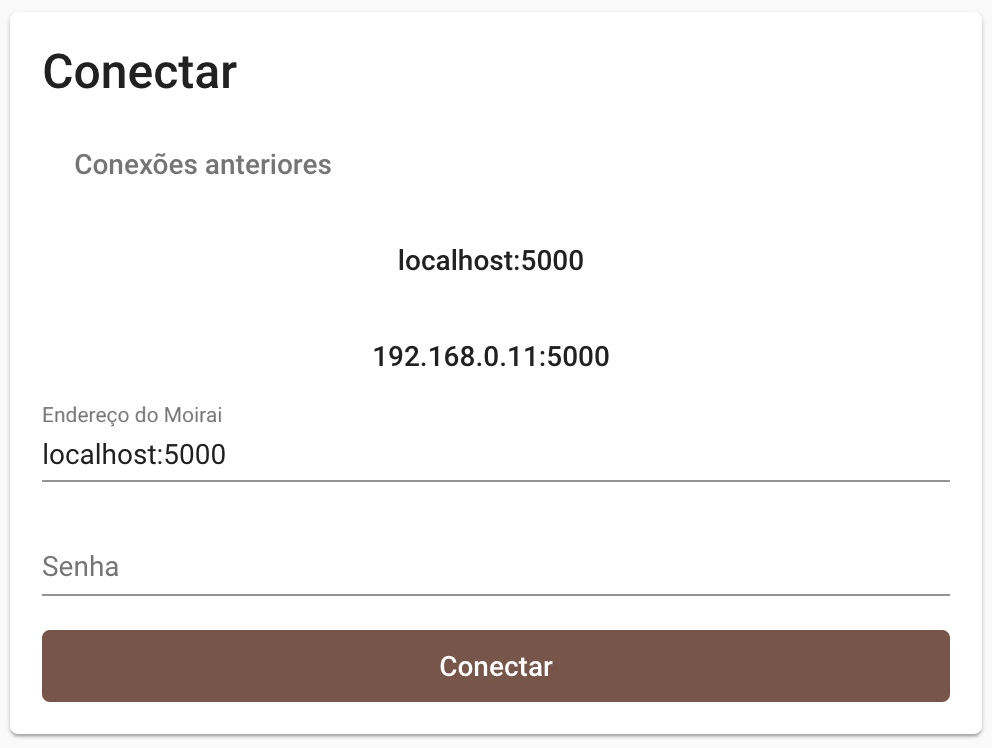
\includegraphics[width=0.9\textwidth]{imgs/connect}
    \caption[Módulo de conexão]{Módulo de conexão}%
    \label{fig:connect}
\end{figure}

Por padrão o endereço \textit{localhost:5000} já vem preenchido. Caso outras
conexões já tenham sido realizadas os endereços serão listados em
\textit{Conexões anteriores}. Basta clicar em um endereço para que ele seja
preenchido no campo correto.

Ao clicar em Conectar algum erro pode ocorrer. Falha de conexão normalmente é
causado por endereço incorreto ou erro na rede. Verifique que o endereço está
certo e que seu computador está de fato na mesma rede que o computador contendo
o \textbf{moirai}. Certifique-se também que o \textbf{moirai} está em execução.
Caso o erro se refira a versão do \textbf{moirai}, esse deve ser atualizado.
Para isso basta executar o comando \mintinline{bash}{pip3 install moirai
--upgrade} em um terminal na máquina onde o \textbf{moirai} se encontra
instalado. Não se esqueça de reiniciar o aplicativo após a atualização.

Uma vez autenticado o módulo de conexão se altera, bem como a barra leteral,
como pode ser visto na Figura~\ref{fig:connection-screen}. A barra lateral exibe
os módulos existentes na plataforma, enquanto o módulo de conexão mostra as
opções de desconectar, alterar senha e salvar/restaurar.

\begin{figure}[ht!]
    \centering
    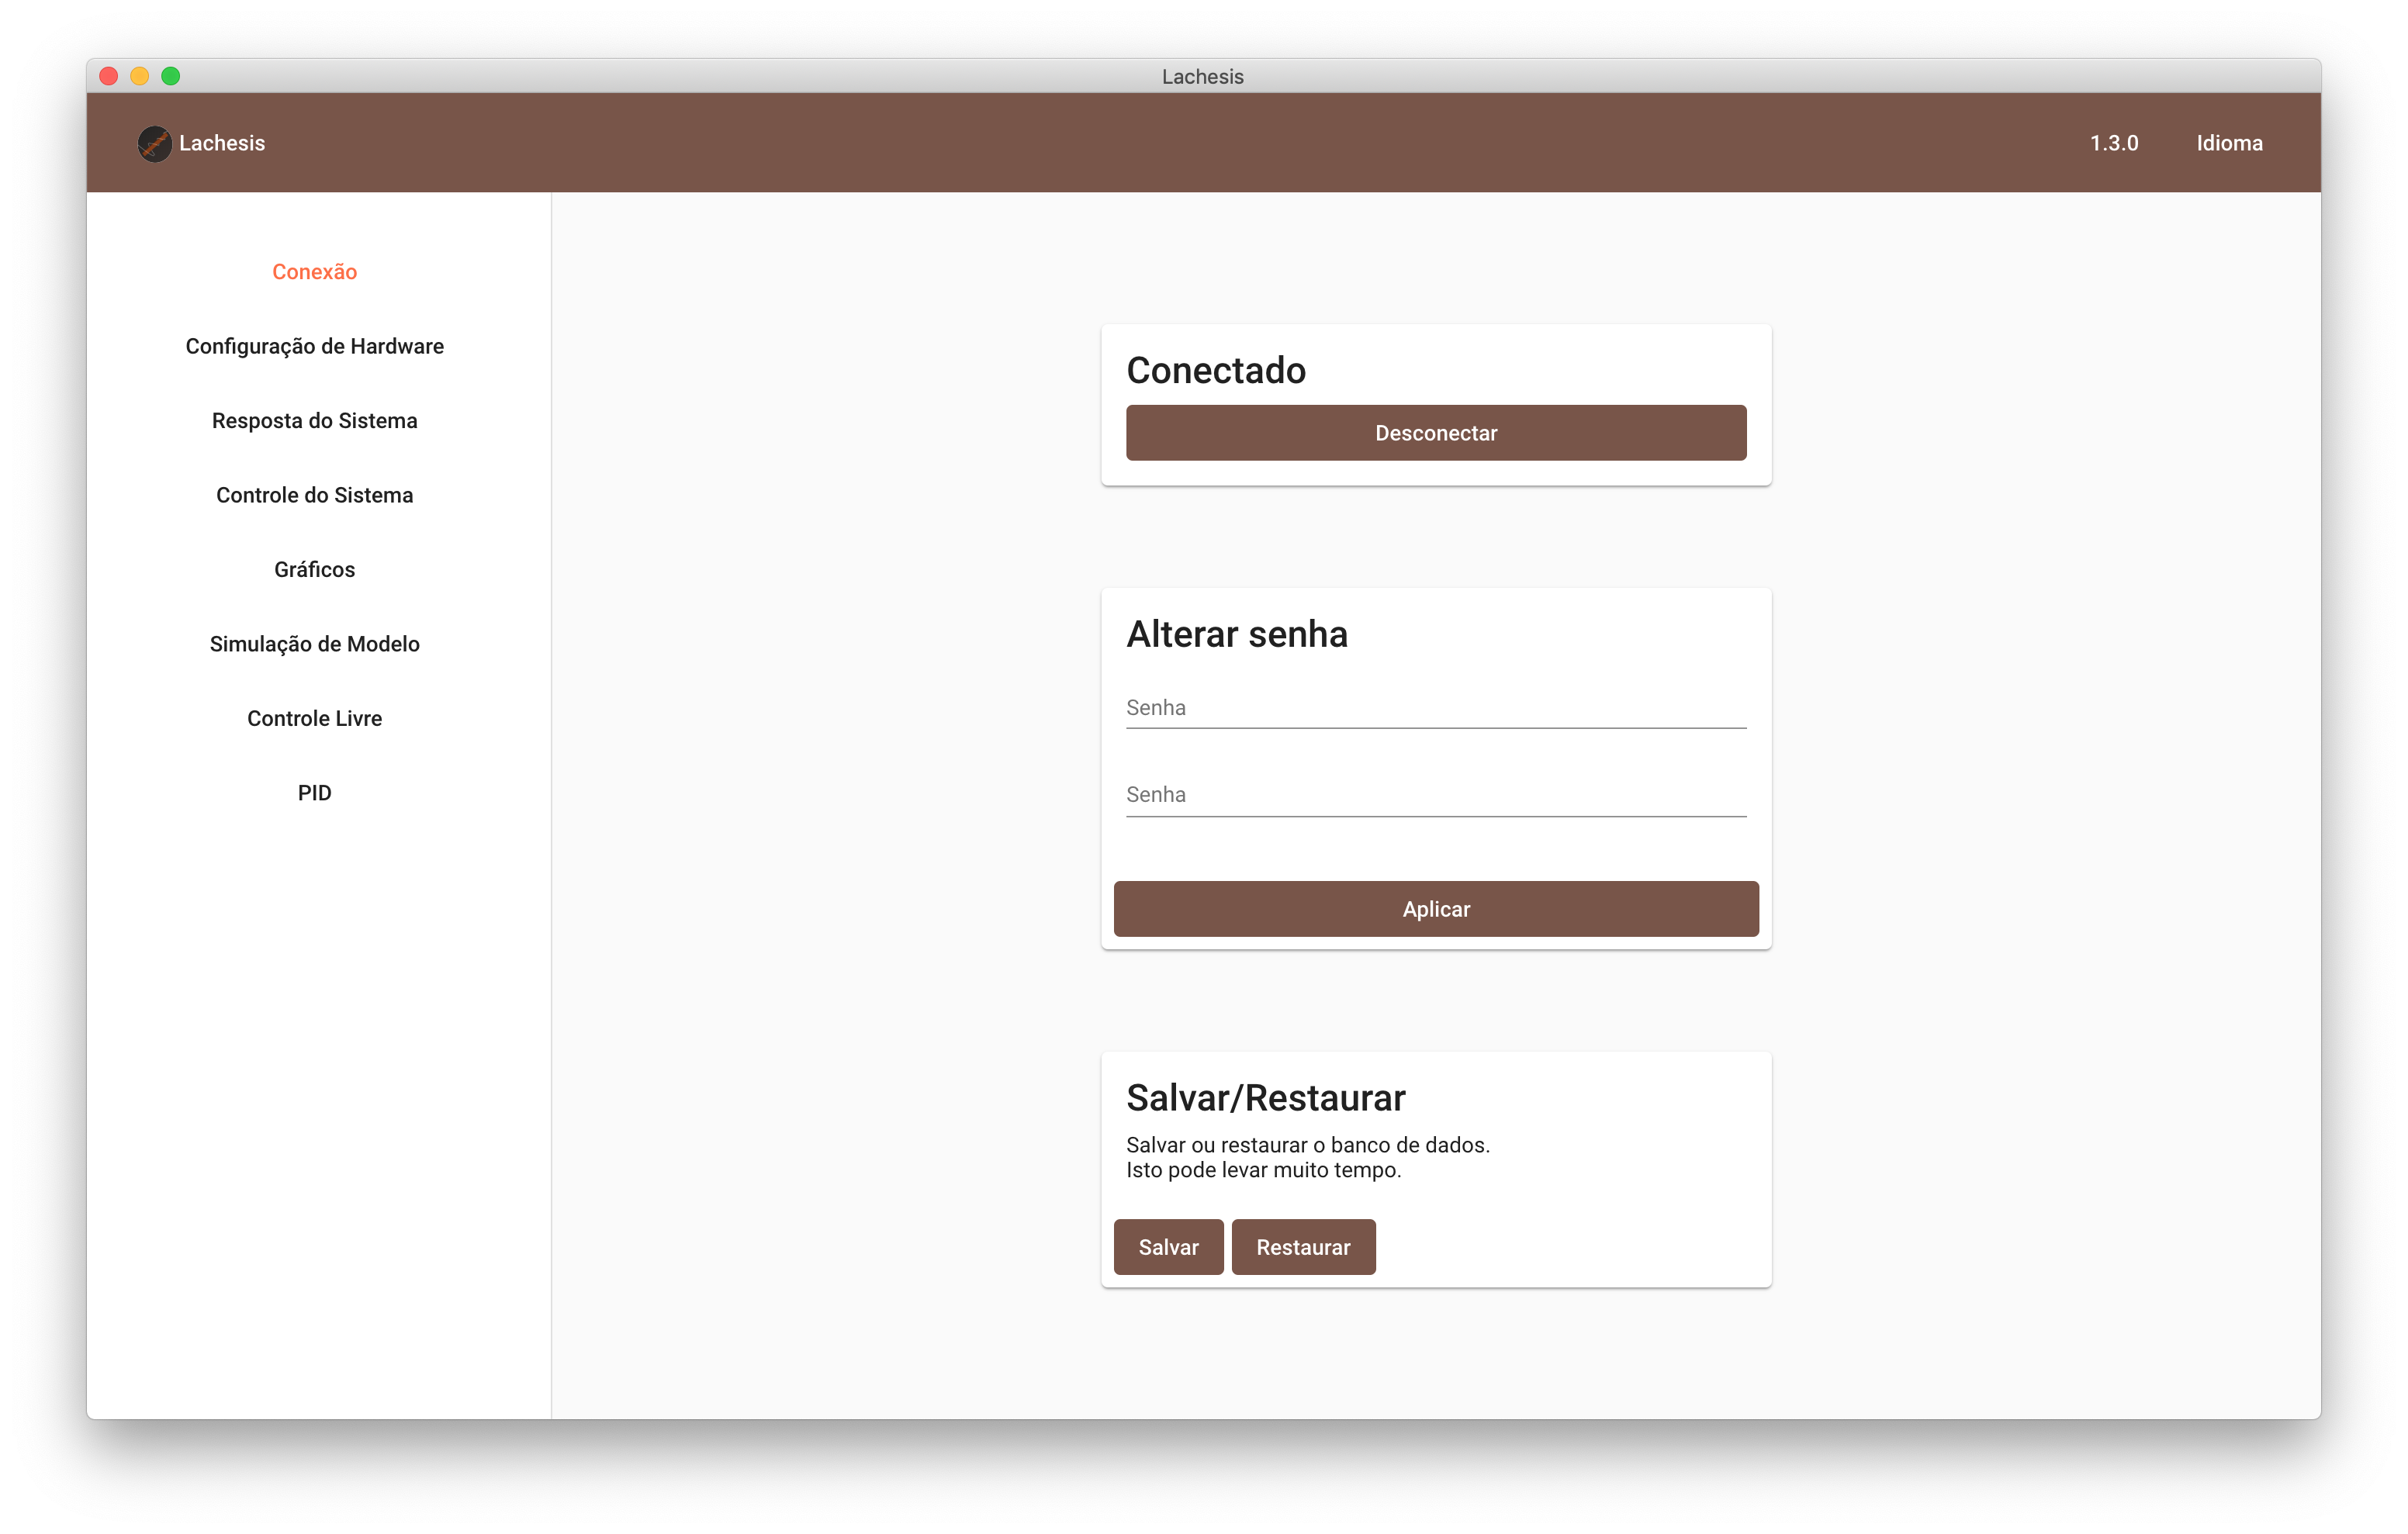
\includegraphics[width=0.9\textwidth]{imgs/connection-screen}
    \caption[Módulo de conexão após autenticação]{Módulo de conexão após autenticação}%
    \label{fig:connection-screen}
\end{figure}

Ao clicar em desconectar o aplicativo volta ao estado inicial, não exibindo os
módulos na lateral e pedindo pelo \textit{IP} e senha.

Para alterar a senha do \textbf{moirai} basta digitar a nova senha duas vezes,
nas duas caixas próprias, e clicar em Aplicar.

As opções Salvar e Restaurar fazem \textit{backup} e restauração de todo o banco
de dados do \textbf{moirai}. Deve-se atentar ao fato que a restauração apaga o
banco atual antes de importar os novos dados, resultando em perda de dados que
não tenham sido salvos em \textit{backup}.

Como o \textit{backup} salva o banco de dados inteiro, os testes realizados
também são salvos. Essa opção pode então ser utilizada para remover dados do
banco, acelerando o aplicativo, sem perder dados. Também pode ser realizada para
migrar o \textbf{moirai} de uma máquina pra outra.

  \cleardoublepage{}
  % !TeX root = document.tex
% !TeX encoding = UTF-8 Unicode

\chapter{Configuração de Hardware}%
\label{chapter:hardware-configuration}

A plataforma foi desenvolvida para se comunicar com qualquer \textit{hardware}.
A comunicação se dá através de \textit{drivers}, escritos em \textit{Python}.
Isso é possível através do projeto
\href{https://github.com/acristoffers/ahio}{AHIO}.

Alguns \textit{drivers} já estão disponíveis por padrão, mas pode-se escrever
novos \textit{drivers} personalizados. Para isso copie o arquivo do
\textit{driver} do \textit{Arduino}
(\href{https://github.com/acristoffers/ahio/blob/master/ahio/drivers/arduino.py}{GitHub})
e modifique para acessar seu \textit{hardware}. Caso necessário, leia os
comentários em
\href{https://github.com/acristoffers/ahio/blob/master/ahio/abstract_driver.py}{abstract\_driver.py}.

Salve o arquivo em algum diretório em seu computador e inicie o \textbf{moirai}
utilizando o seguinte comando:

\mintinline{bash}{AHIO_PATH="/caminho/para/diretorio" moirai}

A variável de ambiente \mintinline{bash}{AHIO_PATH} funciona como a variável
\mintinline{bash}{PATH} dos sistemas \textit{UNIX}.

Os \textit{drivers} padrão são: snap7, Arduino, GenericTCPIO, Raspberry ou
Dummy. Nesse módulo, representada na Figura~\ref{fig:hardware1}, pode-se
configurar o \textit{driver} desejado. Primeiramente deve-se selecionar o
\textit{driver} na lista. Duas seções serão abertas ao selecionar um
\textit{driver}: Configuração e Portas.

\begin{figure}[ht!]
    \centering
    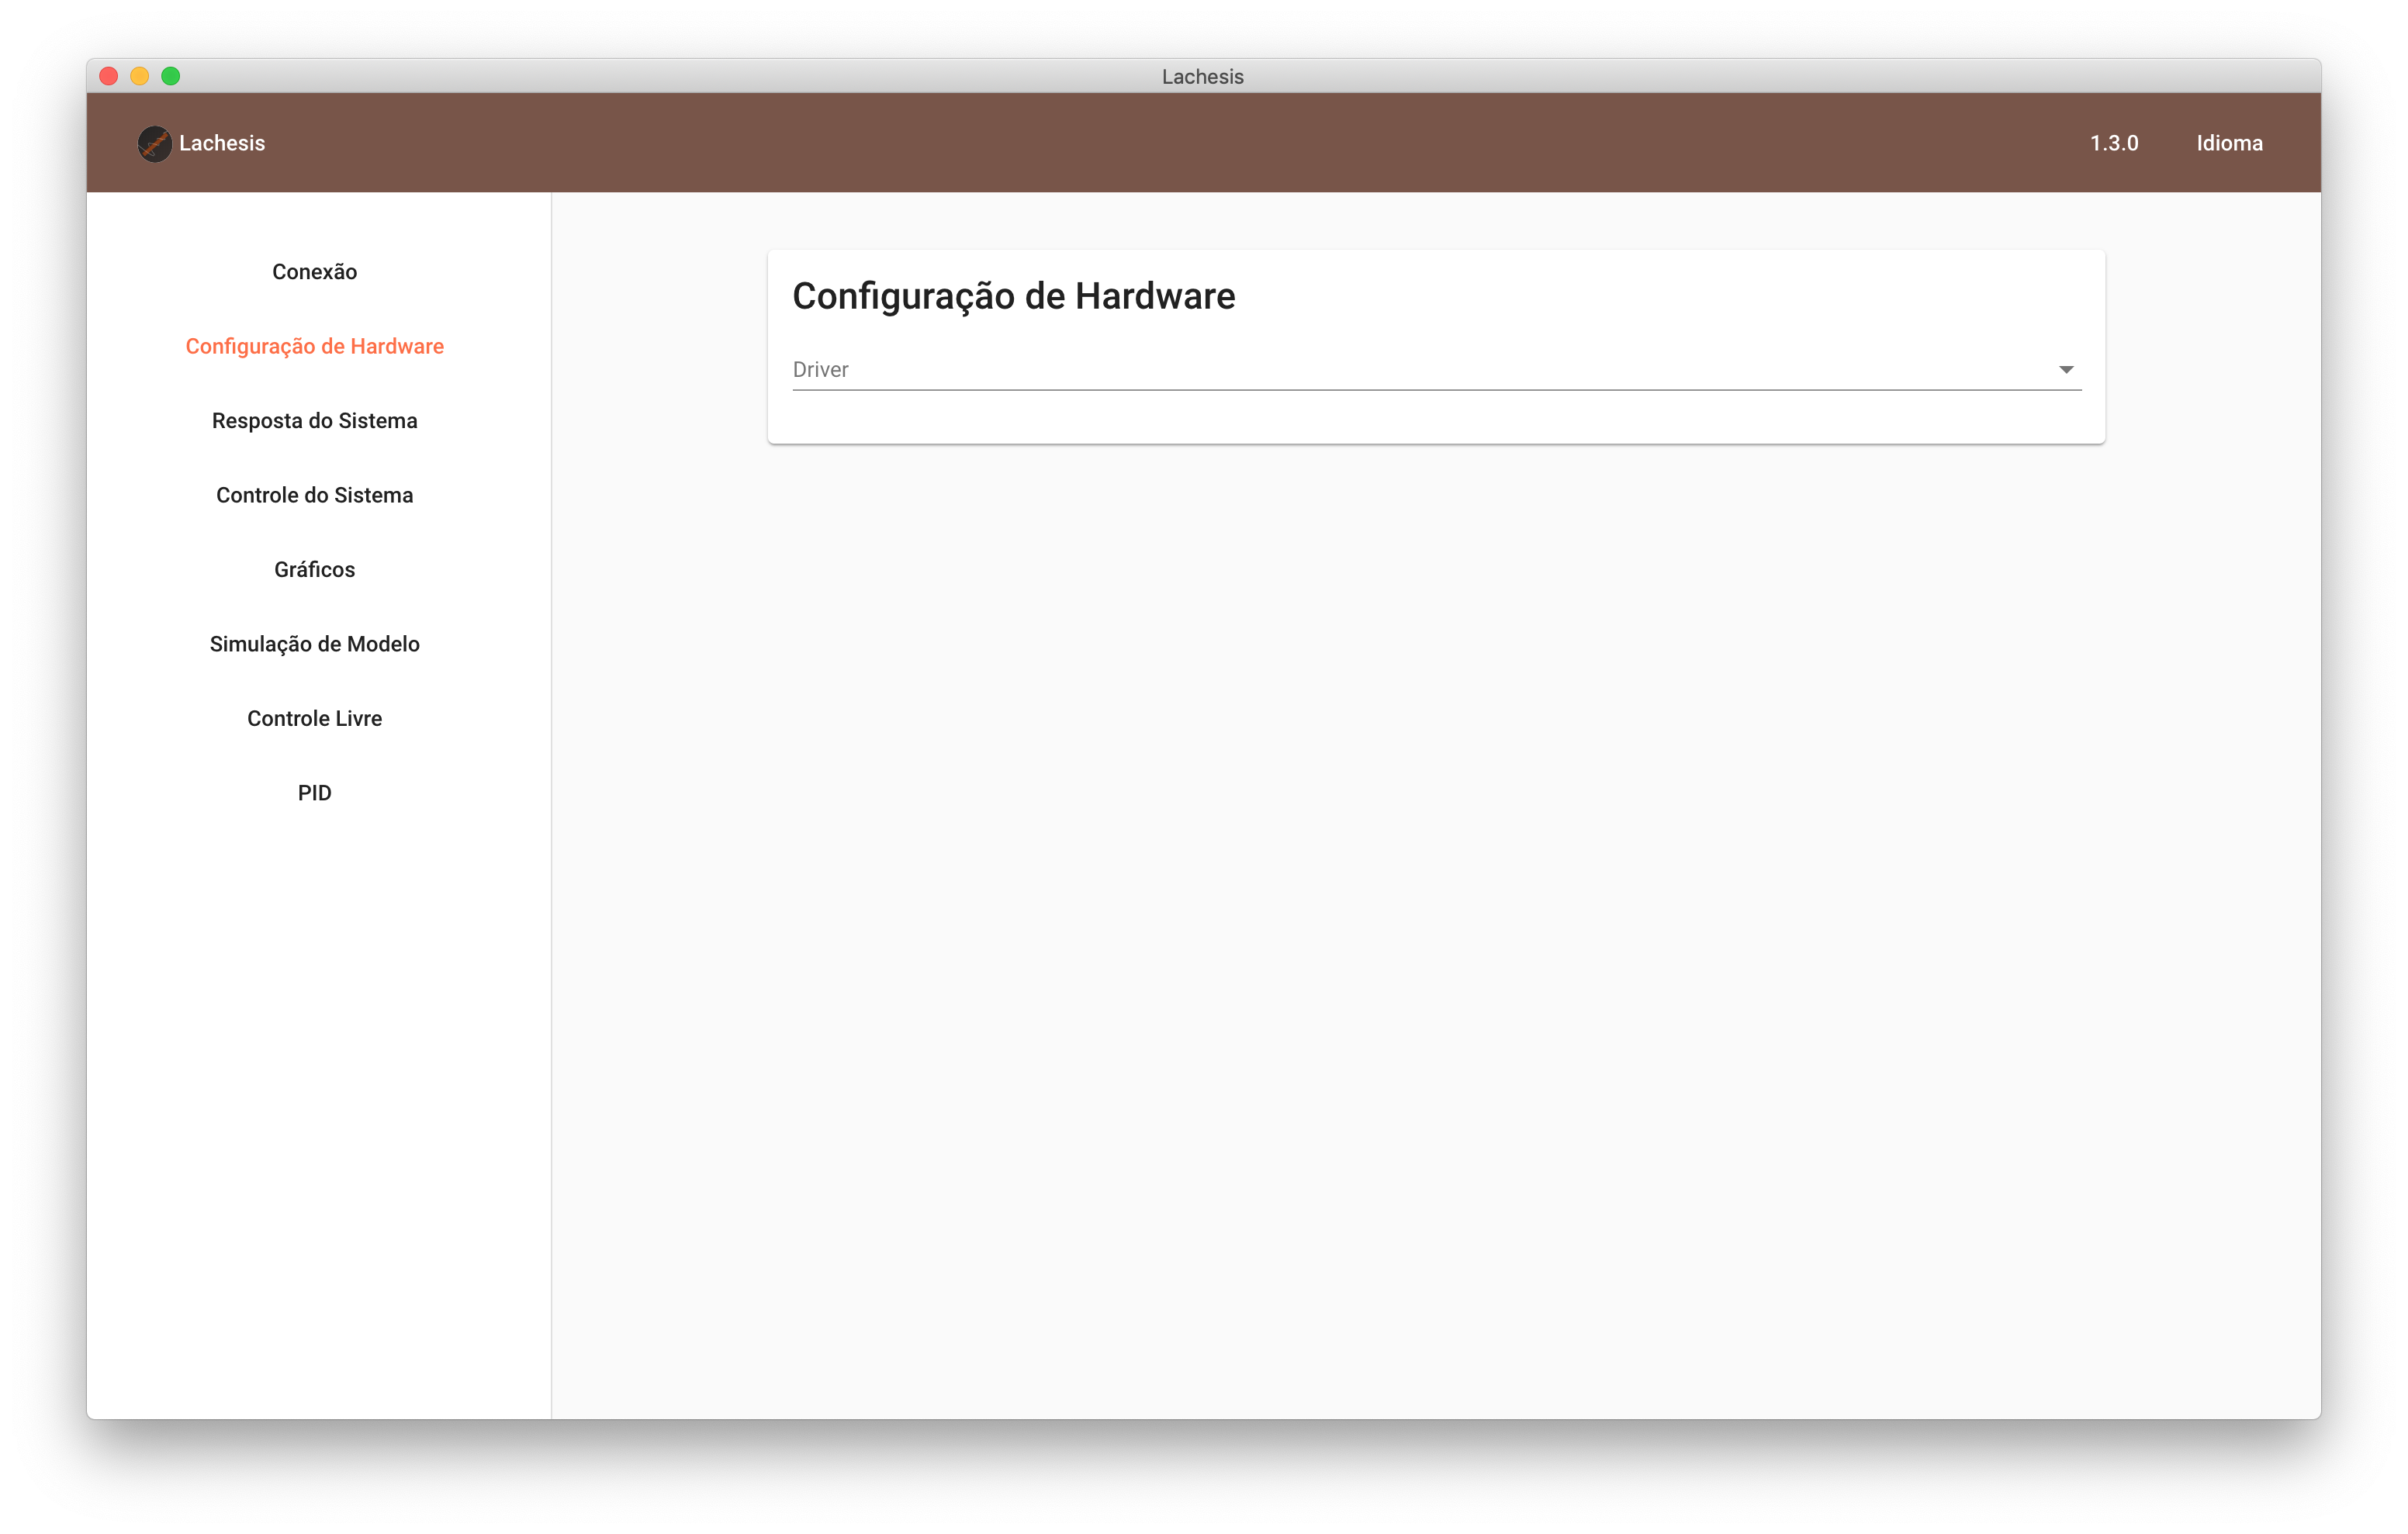
\includegraphics[width=0.9\textwidth]{imgs/hardware}
    \caption[Módulo Hardware sem driver selecionado]{Módulo Hardware sem driver selecionado}%
    \label{fig:hardware1}
\end{figure}

Na seção \textit{Configuração} deve-se inserir a configuração específica do
\textit{driver}. As opções são os parâmetros do método \textit{setup} quando se
utiliza a biblioteca \textit{AHIO} diretamente. Normalmente serão parâmetros de
localização do \textit{hardware}, como porta do \textit{Arduino} ou endereço do
CLP\@.

\begin{figure}[ht!]
    \centering
    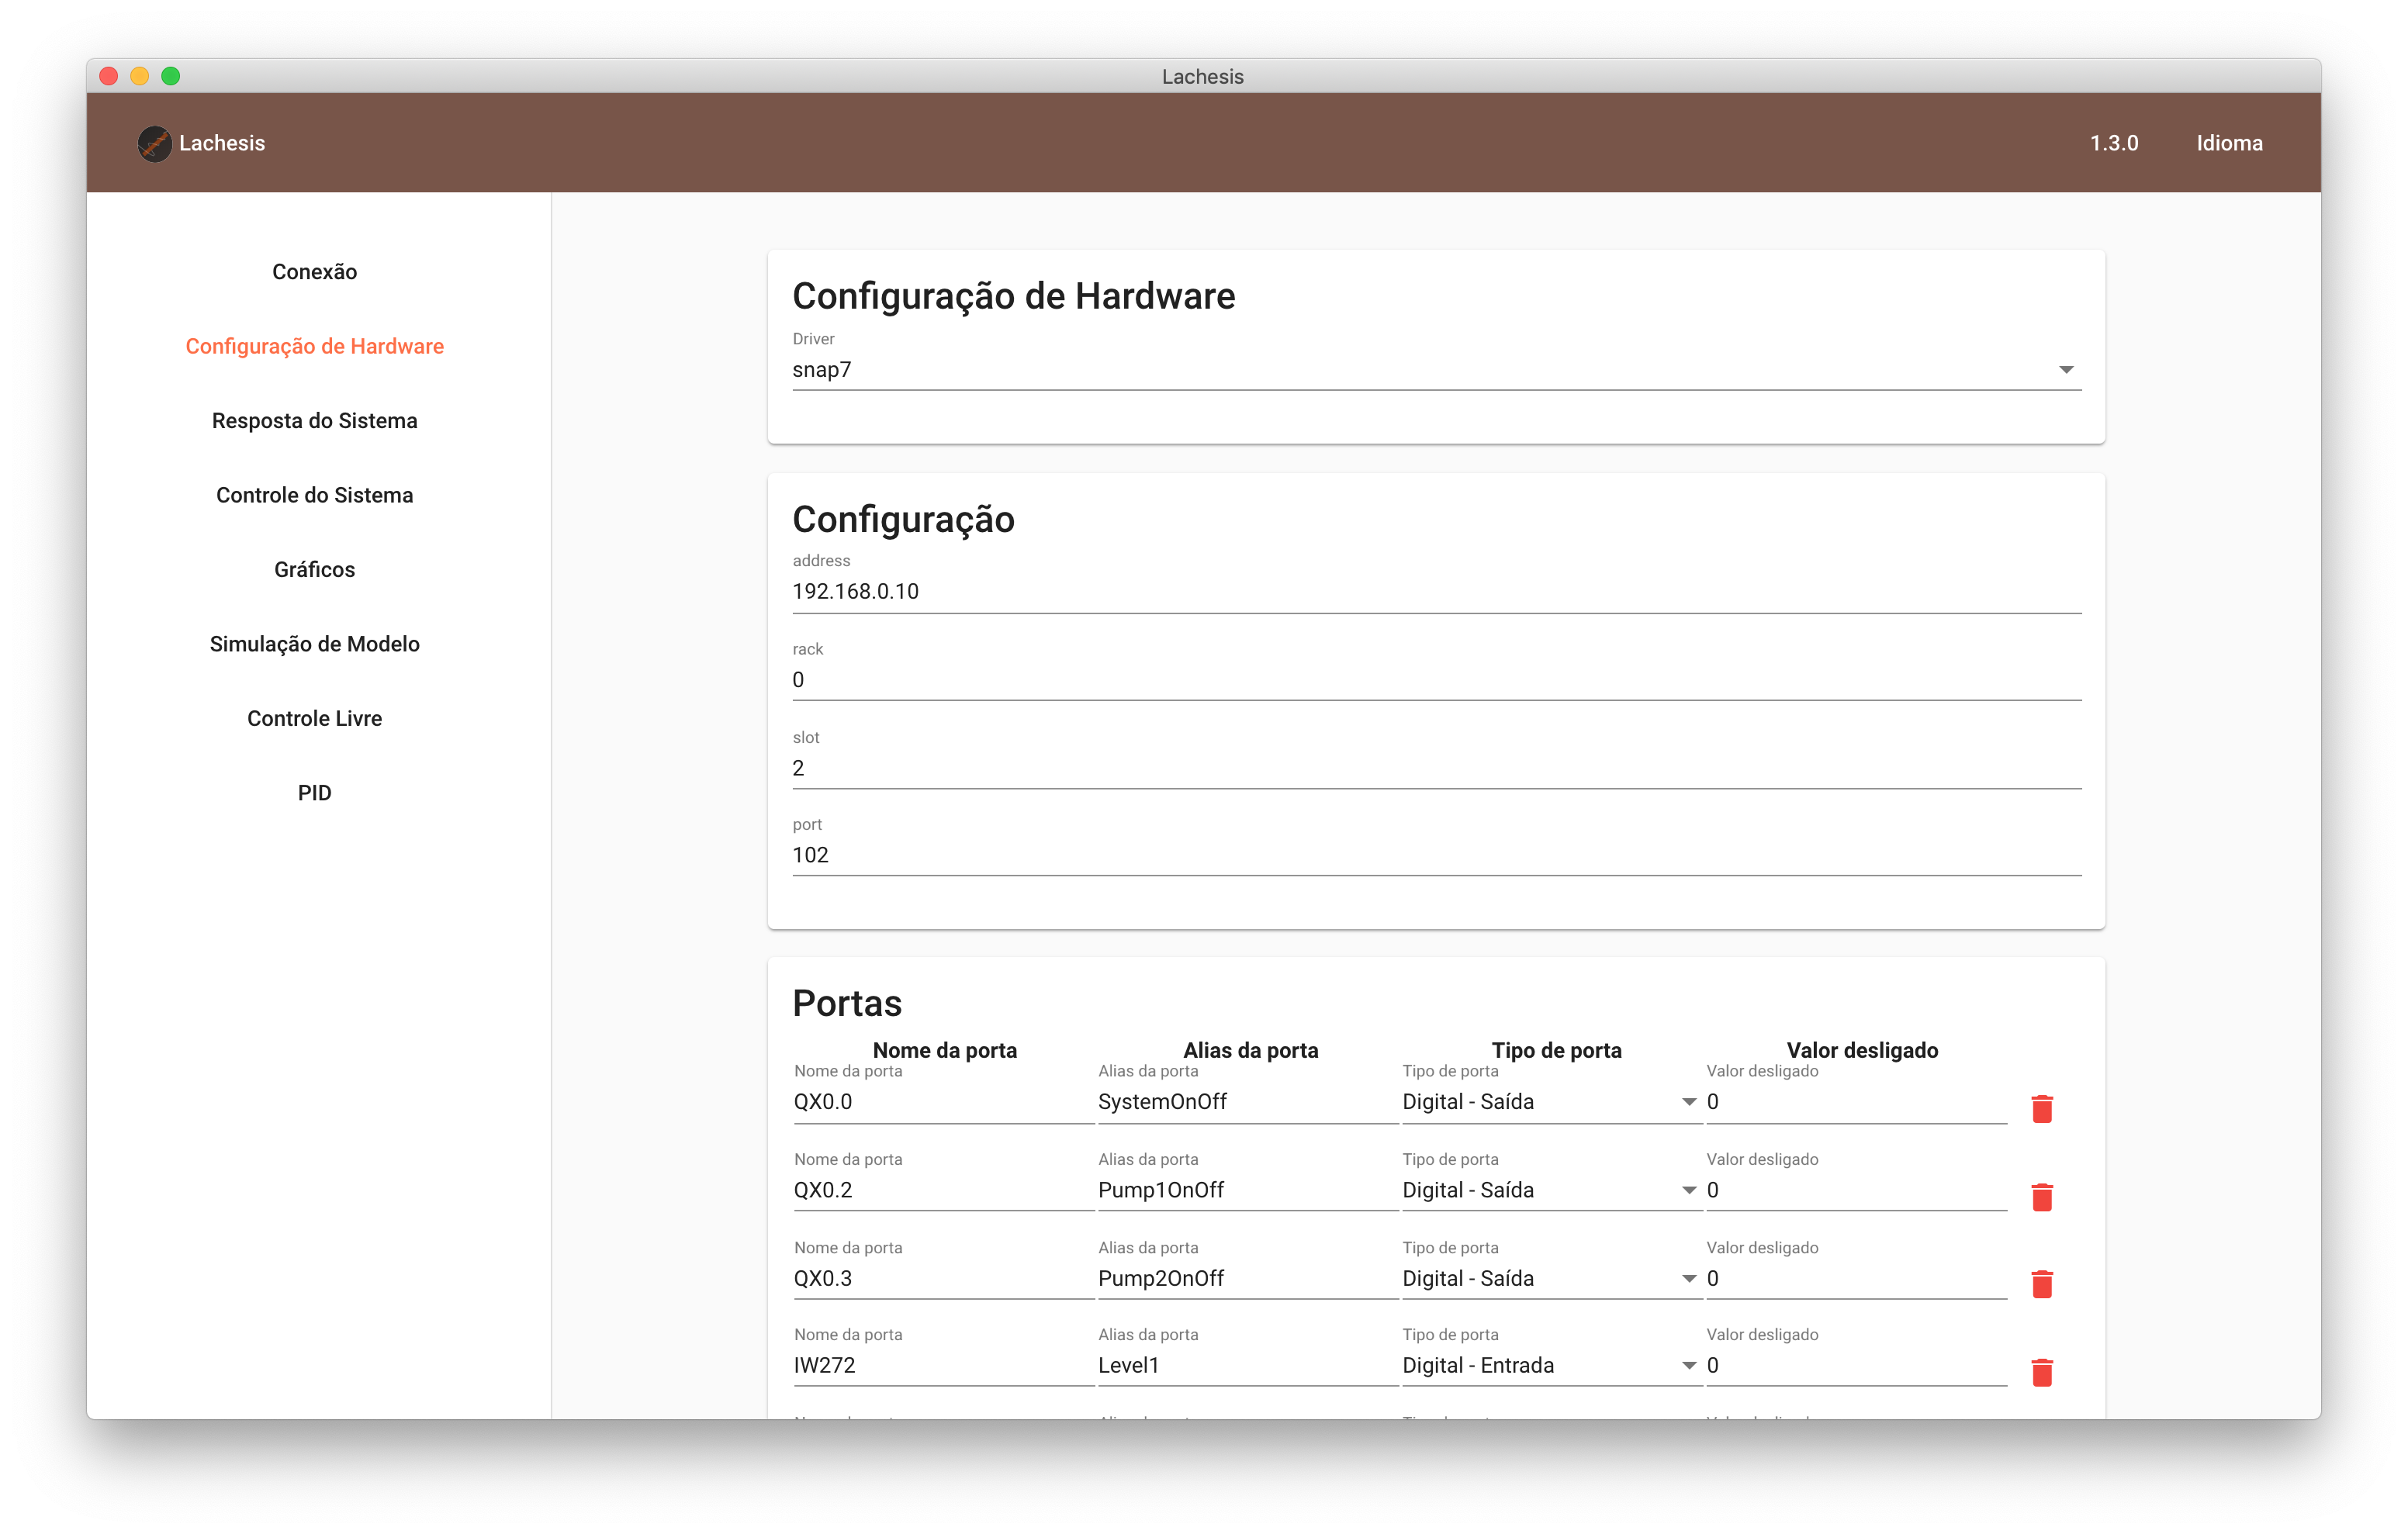
\includegraphics[width=0.9\textwidth]{imgs/hardware2}
    \caption[Módulo Hardware com driver selecionado]{Módulo Hardware com driver selecionado}%
    \label{fig:hardware2}
\end{figure}

A seção \textit{Portas} (Figura~\ref{fig:hardware3}) permite a configuração das
entradas e saídas do sistema. Ao clicar em \textit{Adicionar} uma nova entrada
em branco é inserida. Ela contém as seguintes colunas: Nome da porta, Alias da
porta, Tipo de porta, Valor desligado.

\begin{figure}[ht!]
    \centering
    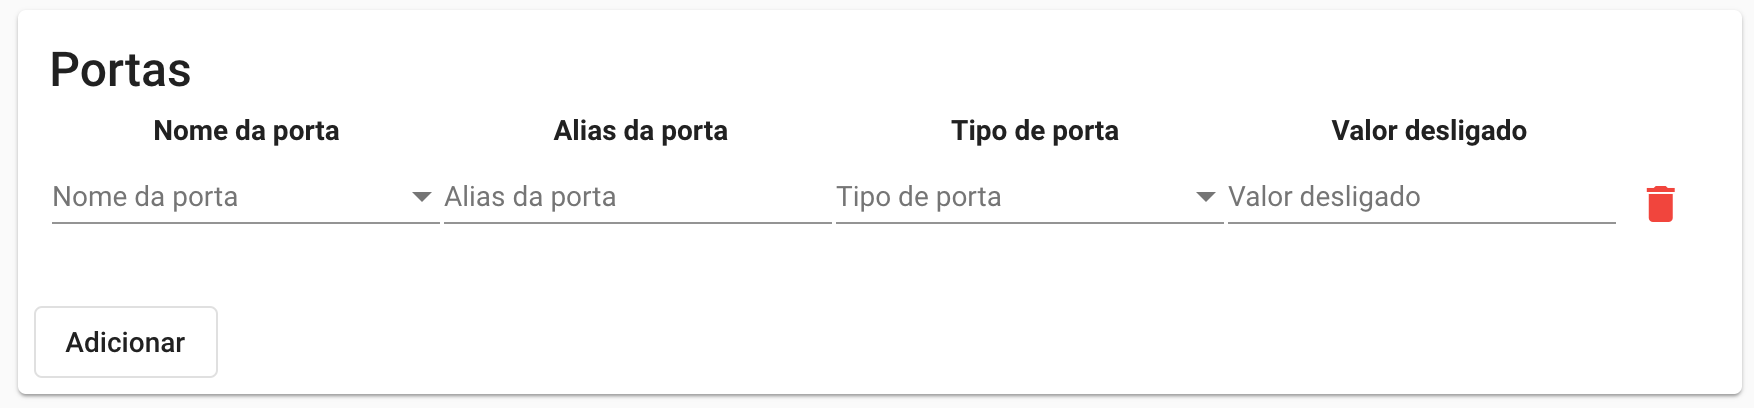
\includegraphics[width=0.9\textwidth]{imgs/hardware3}
    \caption[Seção Portas]{Seção Portas}%
    \label{fig:hardware3}
\end{figure}

O \textit{Nome da porta} pode ser uma caixa de seleção (\textit{dropbox}) ou uma
caixa de texto, a depender do \textit{driver}. No caso do \textit{Arduino}, por
exemplo, será uma \textit{dropbox} com todas as portas do dispotivo. No caso de
um CLP (\textit{driver Snap7}) será uma caixa de texto onde o usuário pode
digitar o nome da \textit{TAG}, como \enquote{QX0.0} ou \enquote{IW292}. Esse
campo referencia a porta física no hardware.

O \textit{Alias da porta} é o nome dado para essa porta física no aplicativo.
Esse nome serve como uma variável e será exibido em formulários e acessado por
código. Escolha um nome que identifique bem o que está ligado à porta. Por
exemplo, num sistema de tanques temos o alias \enquote{Pump1} associado à porta
\enquote{QW272}, pois essa porta irá comandar a bomba número 1 do sistema.

O \textit{Tipo de porta} varia de acordo com a escolha da porta física. Pode ser
uma combinação de digital ou analógica, entrada ou saída. Também pode ser do
tipo saída \textit{PWM}. O \textit{driver} pode limitar as opções disponíveis de
acordo com a porta selecionada.

\textit{Valor desligado} apenas faz sentido para atuadores. É o valor que será
escrito na porta em determinadas situações. Normalmente é utilizado para
desligar o sistema em caso de falhas ou após alguns testes. Se a interface
oferece a opção de definir valores após o teste, essa opção não será usada. Caso
contrário, sim.

Após inserir uma porta, duas novas seções se tornam disponíveis:
\textit{Calibração} e \textit{Intertravamento}.

Na seção \textit{Calibração} (Figura~\ref{fig:hardware4}) pode-se definir funções
de calibração para as portas. No campo \textit{Porta} deve-se selecionar uma das
portas registradas anteriormente. Note que já são listados os \textit{alias}. No
campo \textit{Alias} deve-se definir um novo nome para a porta. Ambas estarão
disponíveis nos formulários e código posteriormente. O campo \textit{Calibração
estática} permite a definição de uma fórmula matemática que ligue as duas
portas.

\begin{figure}[ht!]
    \centering
    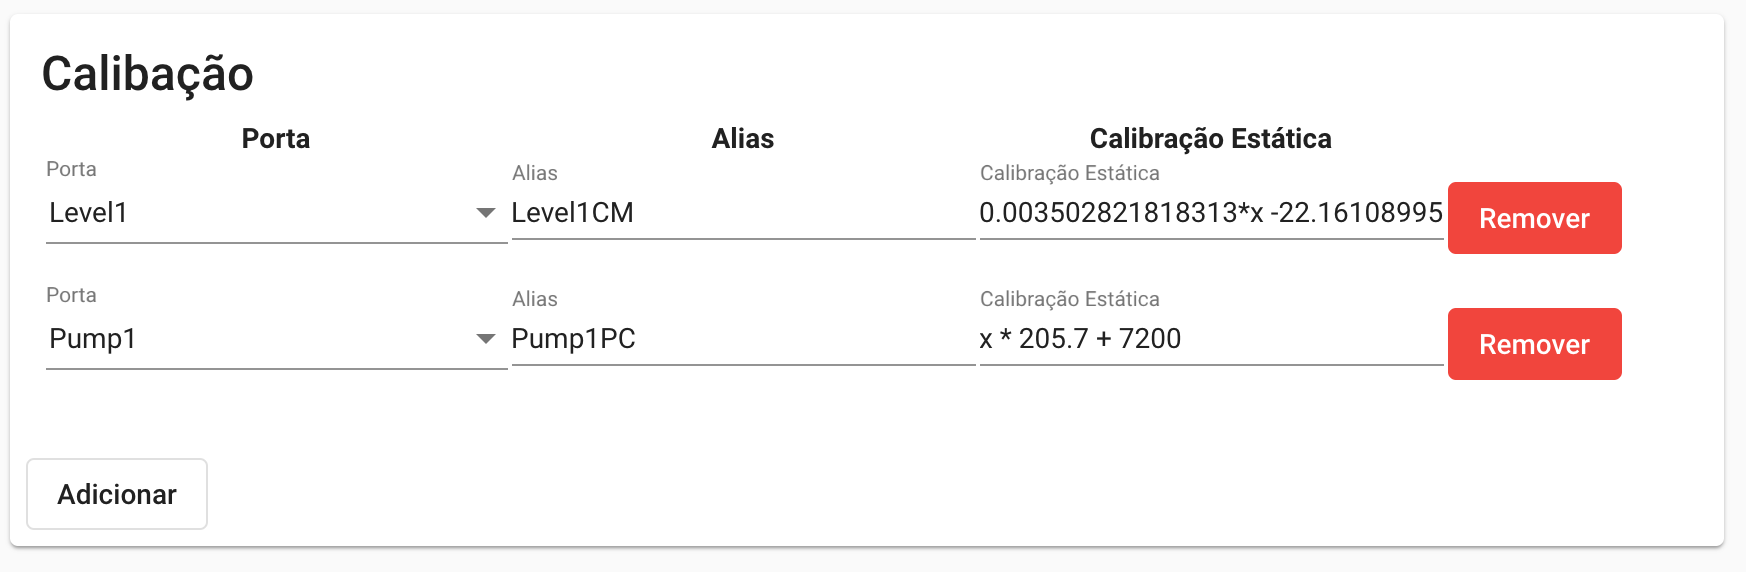
\includegraphics[width=0.9\textwidth]{imgs/hardware4}
    \caption[Seção Calibração]{Seção Calibração}%
    \label{fig:hardware4}
\end{figure}

Como as portas serão ligadas depende se ela é uma entrada ou saída. No caso de
entrada, a nova porta \textit{Alias} recebe o valor da expressão quando se
substitui o valor de x pelo valor da porta selecionada. No caso de saída, o
contrário. Tomando os valores preenchidos como exemplo, temos:

\begin{equation*}
    Level1CM = 0.003502821818313*Level1 -22.161089959823745
\end{equation*}

e

\begin{equation*}
    Pump1 = Pump1PC * 205.7 + 7200.
\end{equation*}

Na seção \textit{Intertravamento} (Figura~\ref{fig:hardware5}) é possível
configurar expressões que, quando verdadeiras, irão definir o valor de outra
variável, além de parar o teste. Exemplo disso é o intertravamento em um sistema
de tanques comunicantes, caso o nível de água ultrapasse 70 centímetros, o teste
é parado e a variável \textit{SystemOnOff} assume valor zero, desligando o
sistema.

\begin{figure}[ht!]
    \centering
    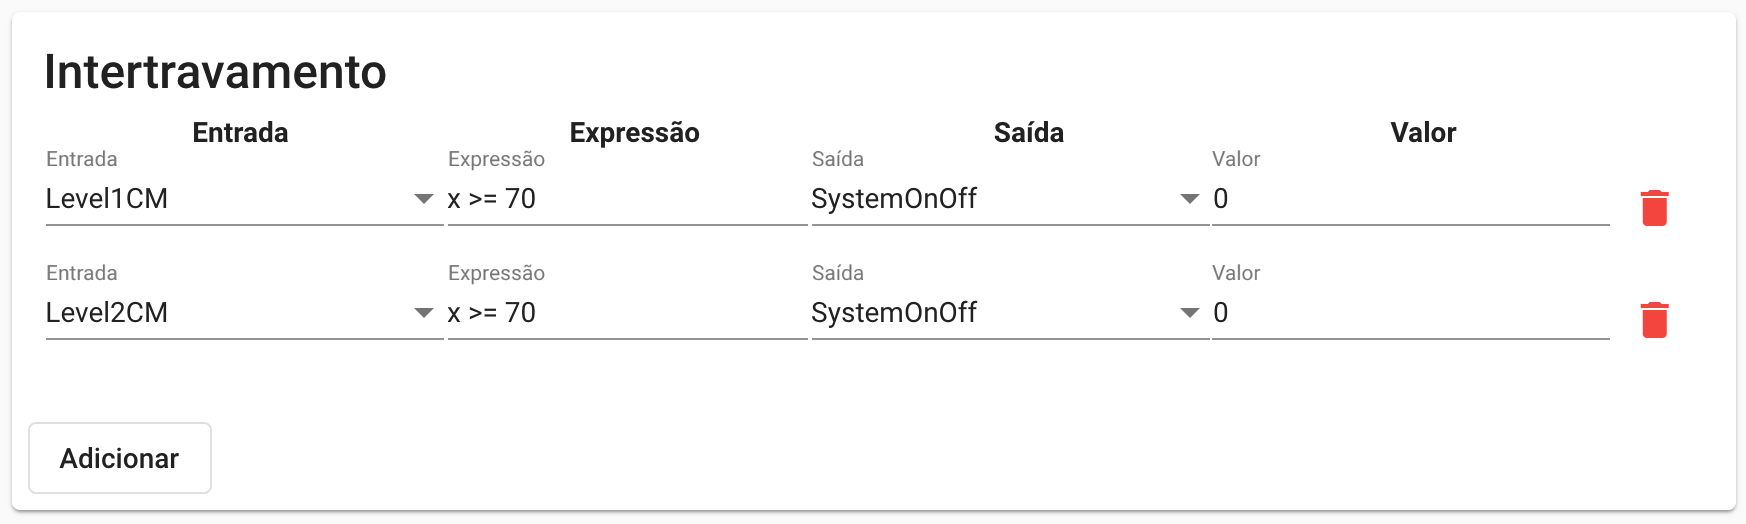
\includegraphics[width=0.9\textwidth]{imgs/hardware5}
    \caption[Seção Intertravamento]{Seção Intertravamento}%
    \label{fig:hardware5}
\end{figure}

No final há opções de exportar/importar configurações de \textit{hardware}
para/de um arquivo, possibilitando o \textit{backup} apenas das configurações do
\textit{driver} ou o compartilhamento de configurações entre pessoas. O botão
\textit{Reinicializar} reinicializa o formulário, sem salvar as alterações. Para
salvar uma configuração nova é necessário clicar na opção \textit{Aplicar}.
Nenhuma configuração será salva se esse botão não for pressionado.

  \cleardoublepage{}
  % !TeX root = document.tex
% !TeX encoding = UTF-8 Unicode

\chapter{Resposta do Sistema}%
\label{chapter:system-response}

Nesse módulo são feitas as configurações de teste em malha aberta. O nome do
módulo remete ao fato que ele permite obter a resposta do sistema à um sinal de
entrada. Na Figura~\ref{fig:system-response1} pode-se ver a lista de testes
configurados, bem como as opções de gerenciar tais testes.

\begin{figure}[ht!]
    \centering
    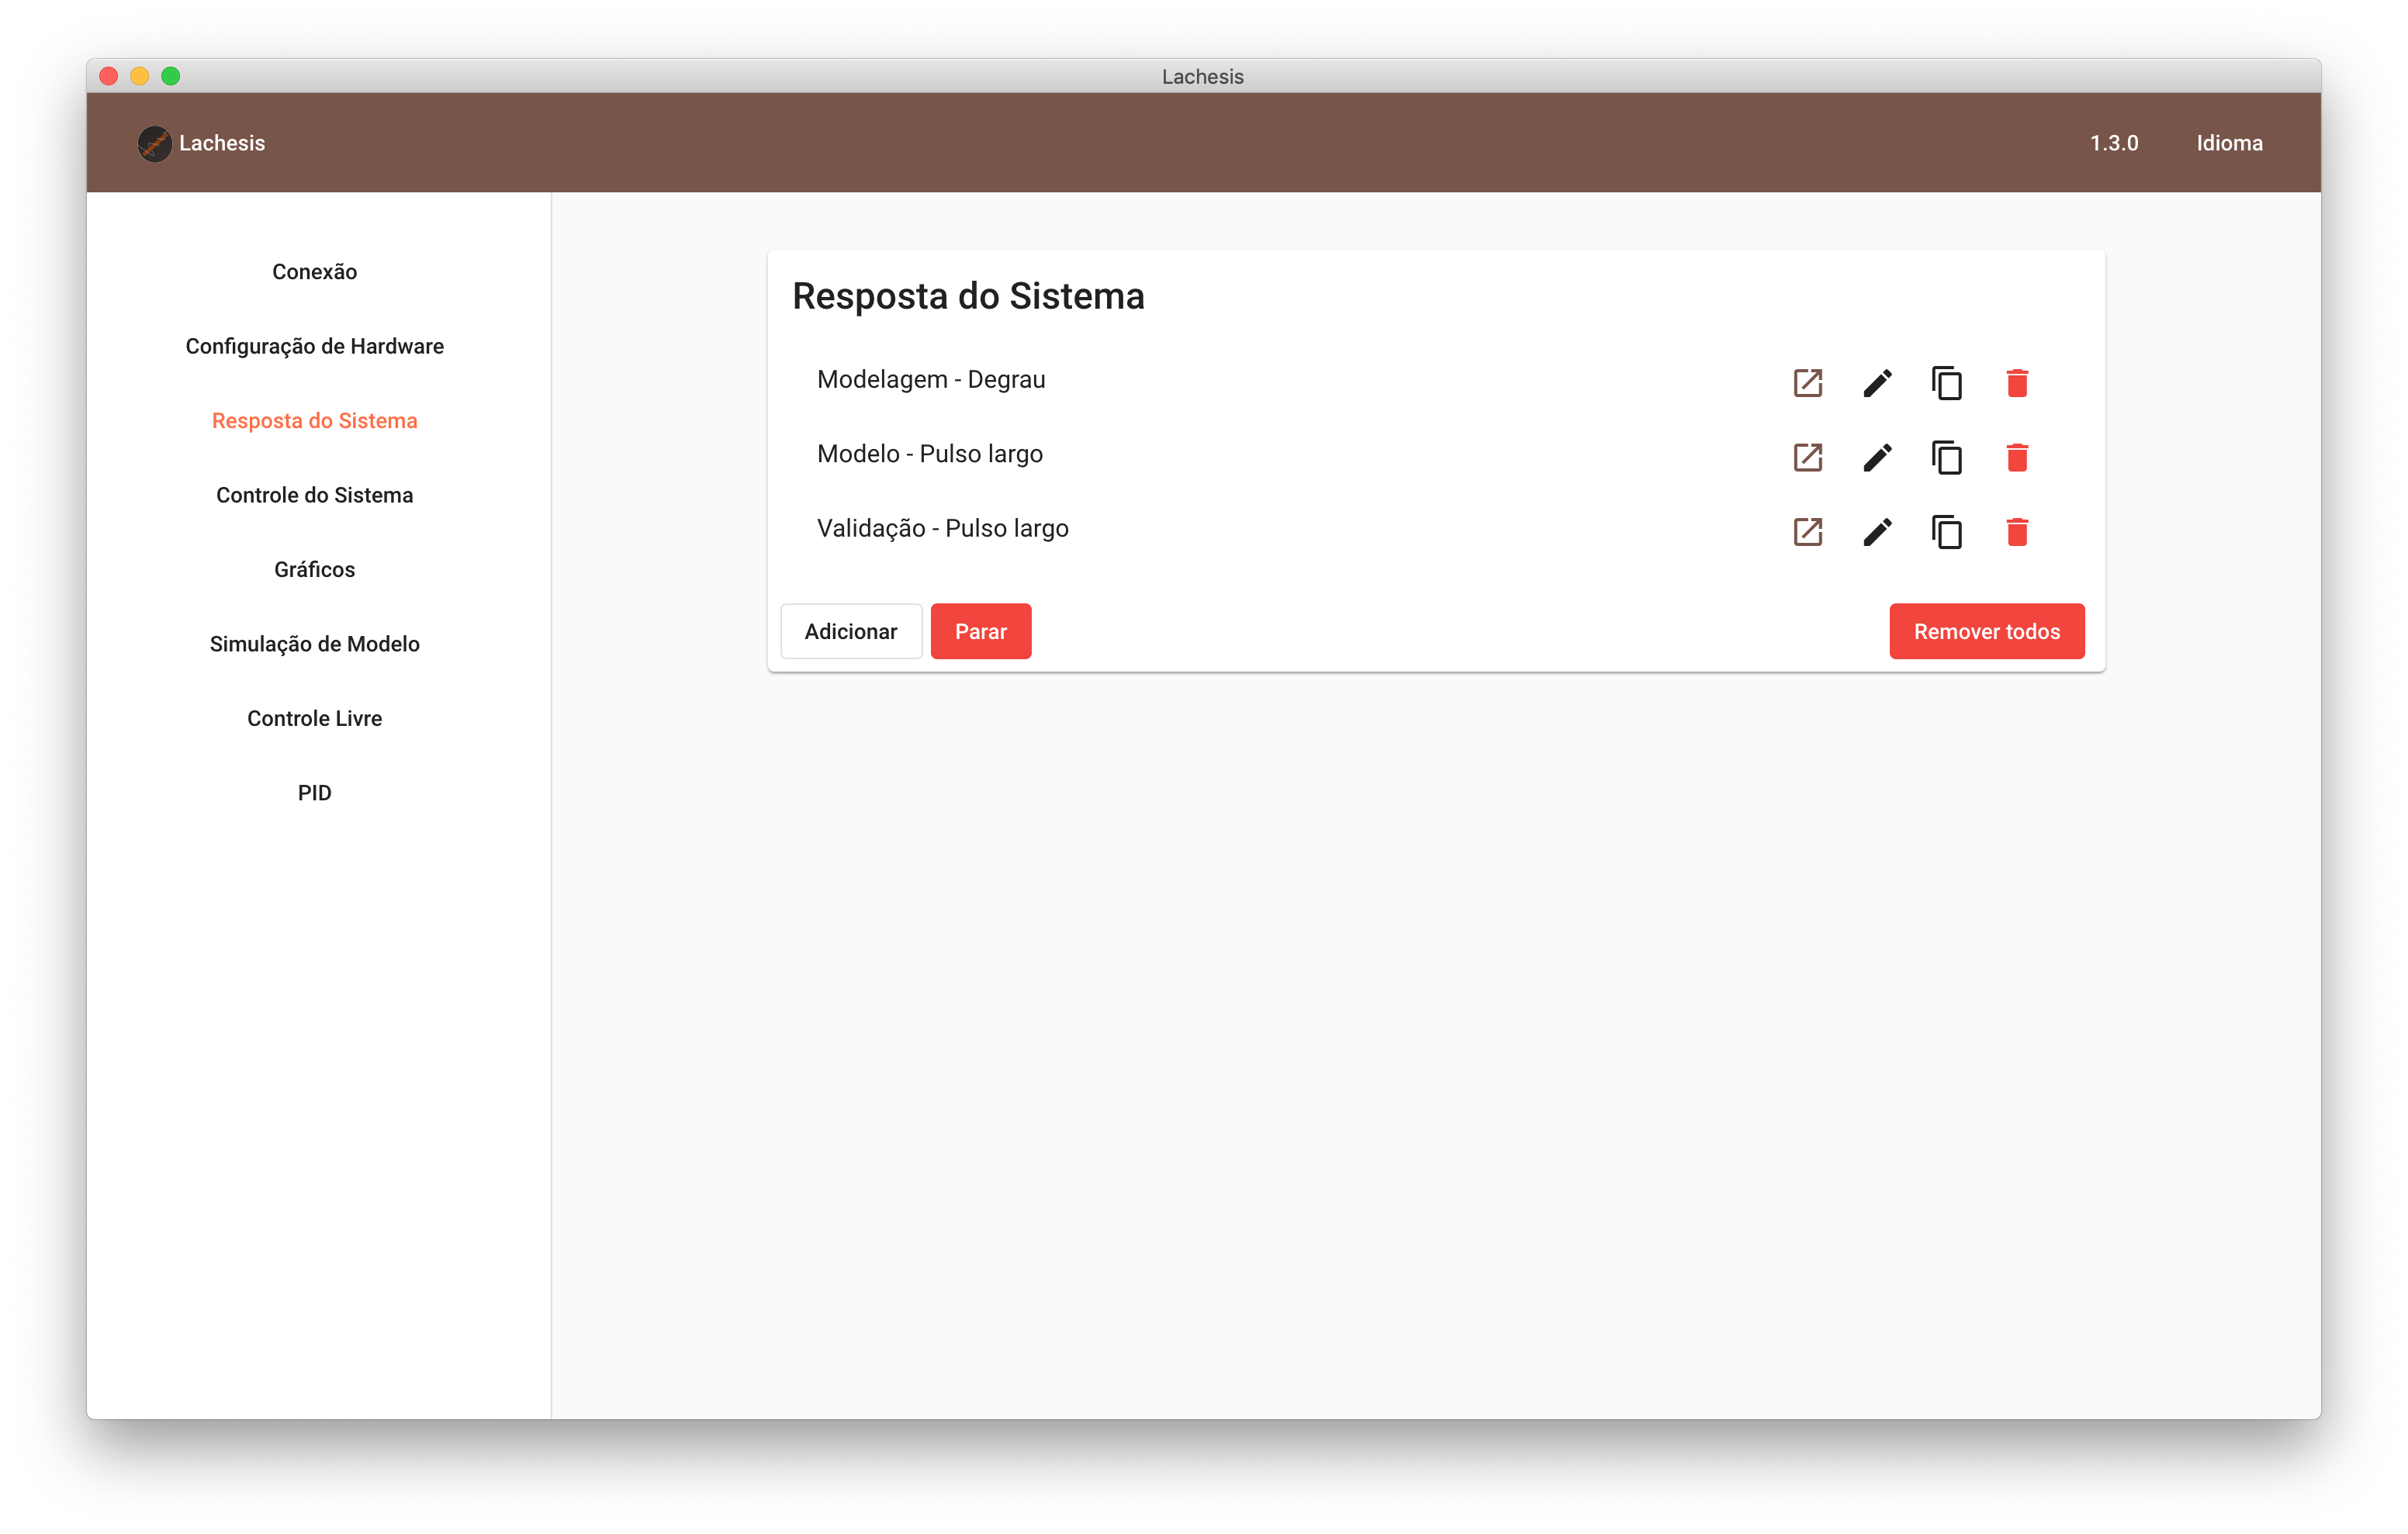
\includegraphics[width=0.9\textwidth]{imgs/system-response1}
    \caption[Módulo Resposta do Sistema]{Módulo Resposta do Sistema}%
    \label{fig:system-response1}
\end{figure}

O botão \textit{Clonar} cria uma cópia do teste. Essa opção é útil para criar
vários testes que possuem apenas pequenas diferenças entre si. O botão
\textit{Executar} inicia o teste e navega para o módulo \textit{Gráficos}.

Ao adicionar ou editar um teste é possível criar várias formas de onde
facilmente, apenas preenchendo um formulário. Cada opção será detalhada nas
seções a seguir. Algumas configurações são comuns e serão na
seção~\ref{sec:step}.

\section{Degrau}%
\label{sec:step}

Todo teste tem um nome. O nome do teste, juntamente com sua data de execução,
serão exibidos na lista de gráficos, onde pode-se ver os gráficos e exportar os
dados (Ver Capítulo~\ref{chapter:graficos}). Portanto, escolha um nome que
permita identificar o motivo de tal teste ter sido realizado e/ou os parâmetros
que foram usados em sua execução. Em um ambiente onde mais de uma pessoa utiliza
o mesmo sistema, também é boa prática colocar seu nome no teste.

Na aba \textit{Degrau}, mostrada na Figura~\ref{fig:system-response2}, é
possível definir um sinal desse tipo. Para isso deve-se informar o valor inicial
\textit{\(V_0\)}, o acréscimo \textit{\(\Delta{}V\)}, que será somado ao valor
inicial após \textit{\(T_0\)} segundos, e o tempo \textit{\(T_1\)} que o sinal
\textit{\(V_0 + \Delta{}V\)} ficará aplicado.

\begin{figure}[ht!]
    \centering
    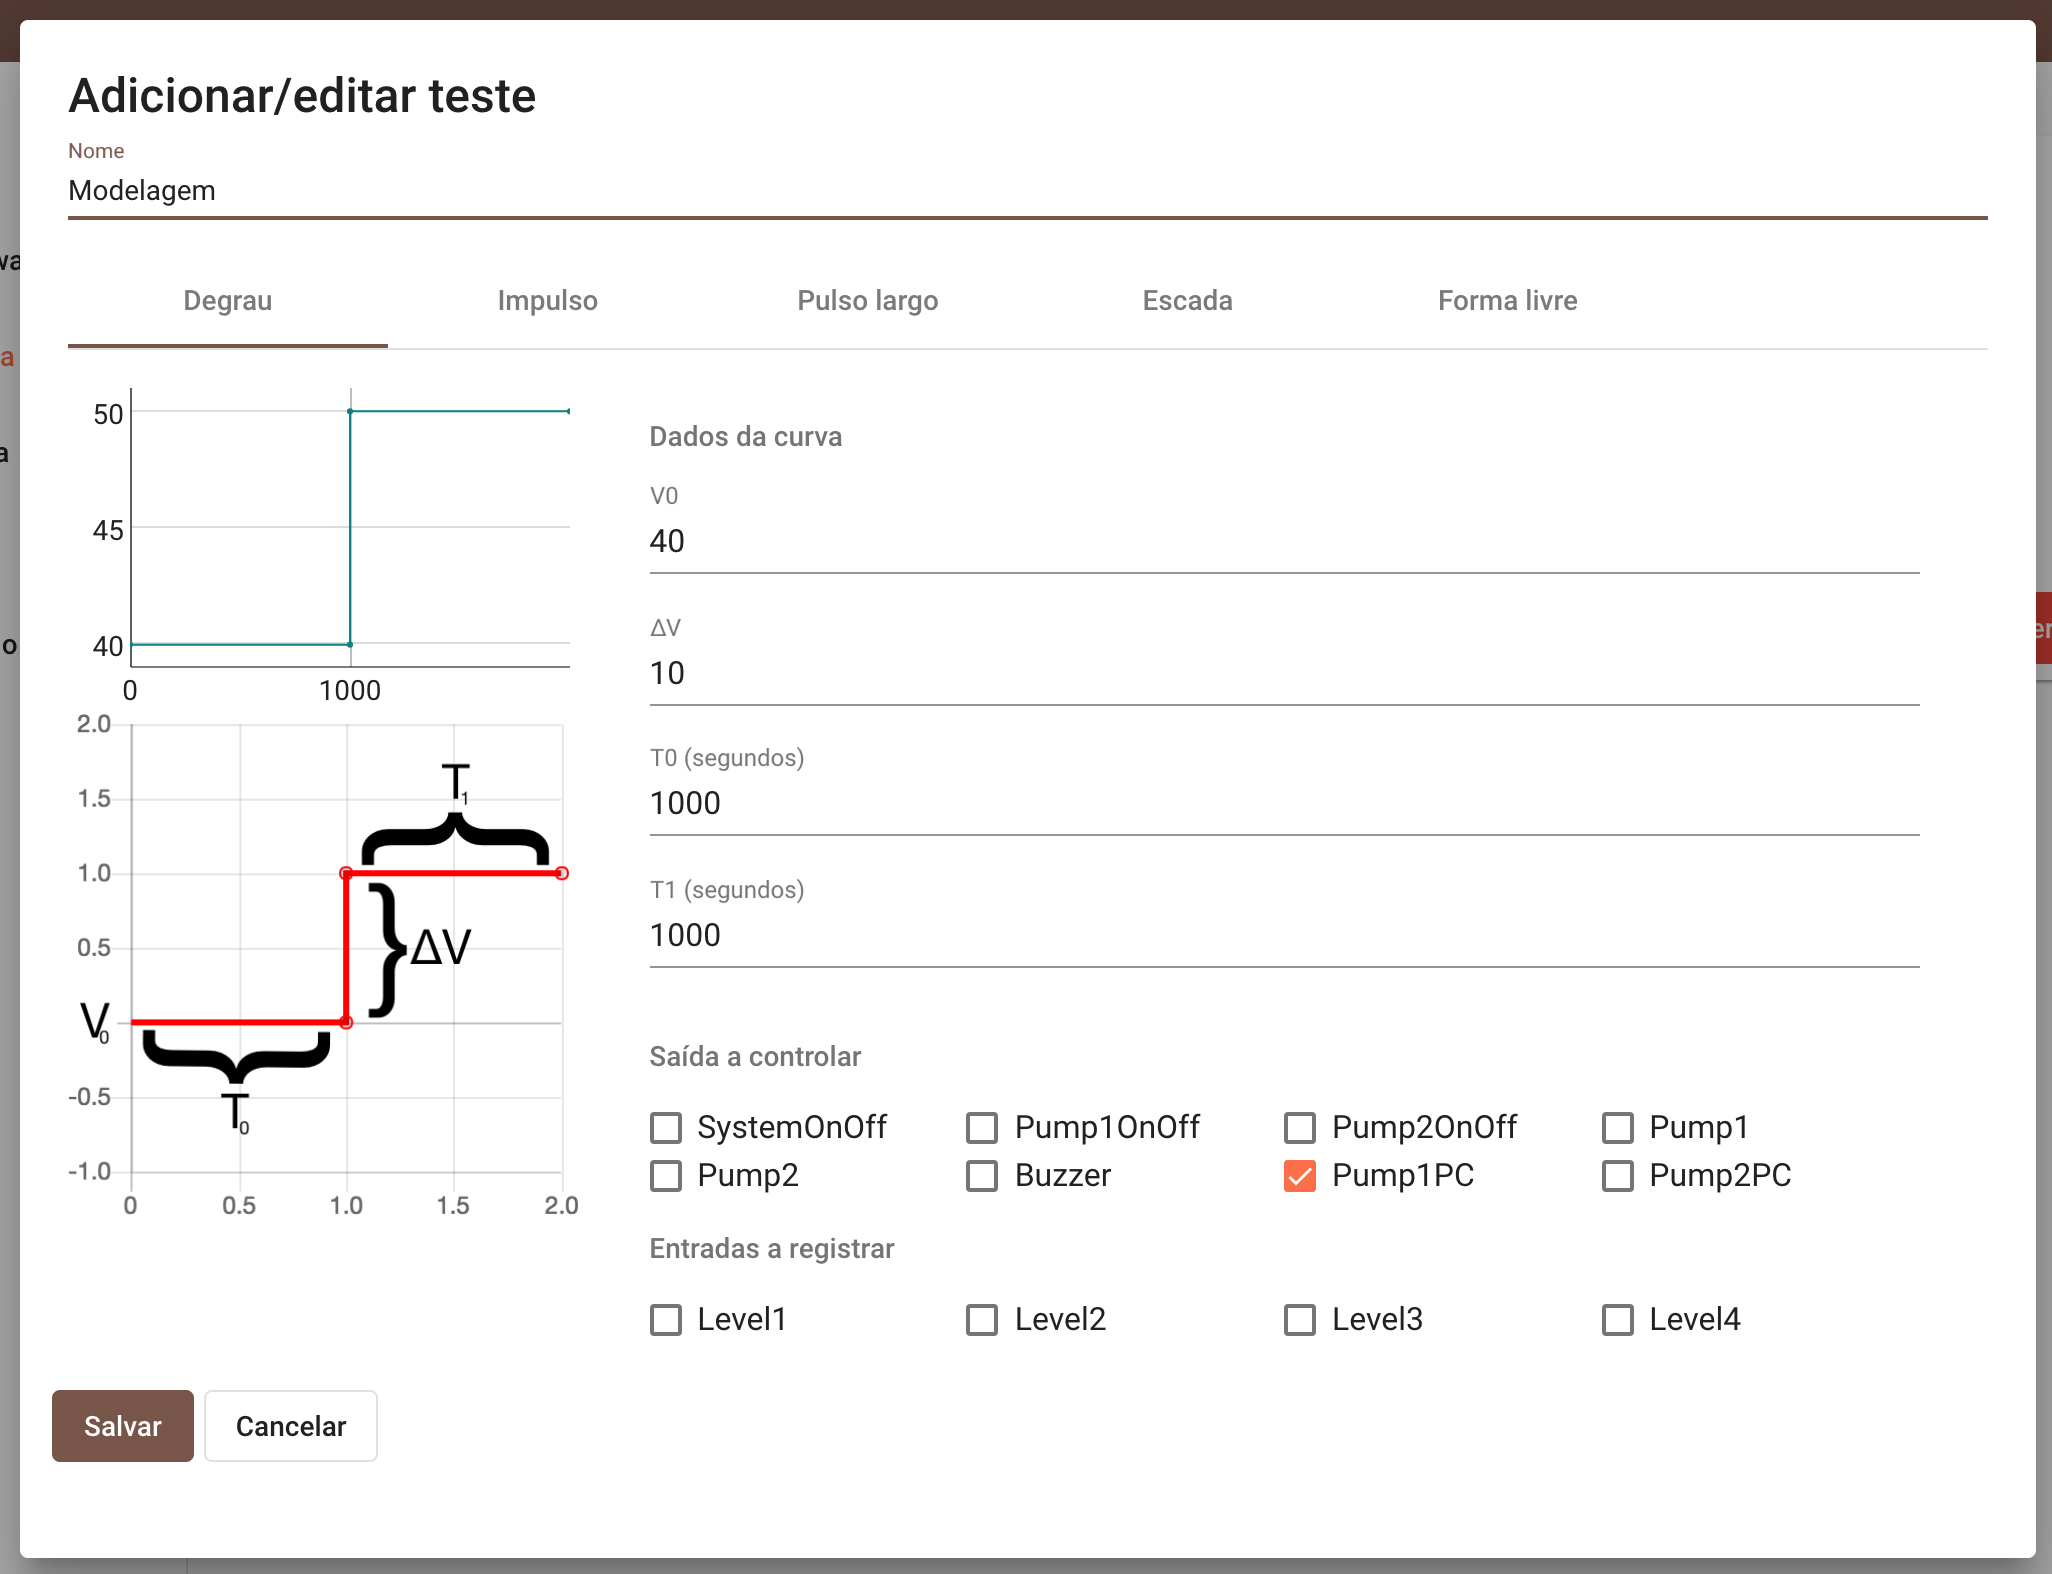
\includegraphics[width=0.9\textwidth]{imgs/system-response2}
    \caption[Sinal do tipo degrau]{Sinal do tipo degrau}%
    \label{fig:system-response2}
\end{figure}

A seção \textit{Configuração de entrada/saída} permite escolher em quais
atuadores o sinal descrito será aplicado. É possível escolher mais de um
atuador, mas todos receberam o mesmo sinal. Também deve-se escolher quais
entradas serão registradas, como mostrado na Figura~\ref{fig:system-response3}.

\begin{figure}[ht!]
    \centering
    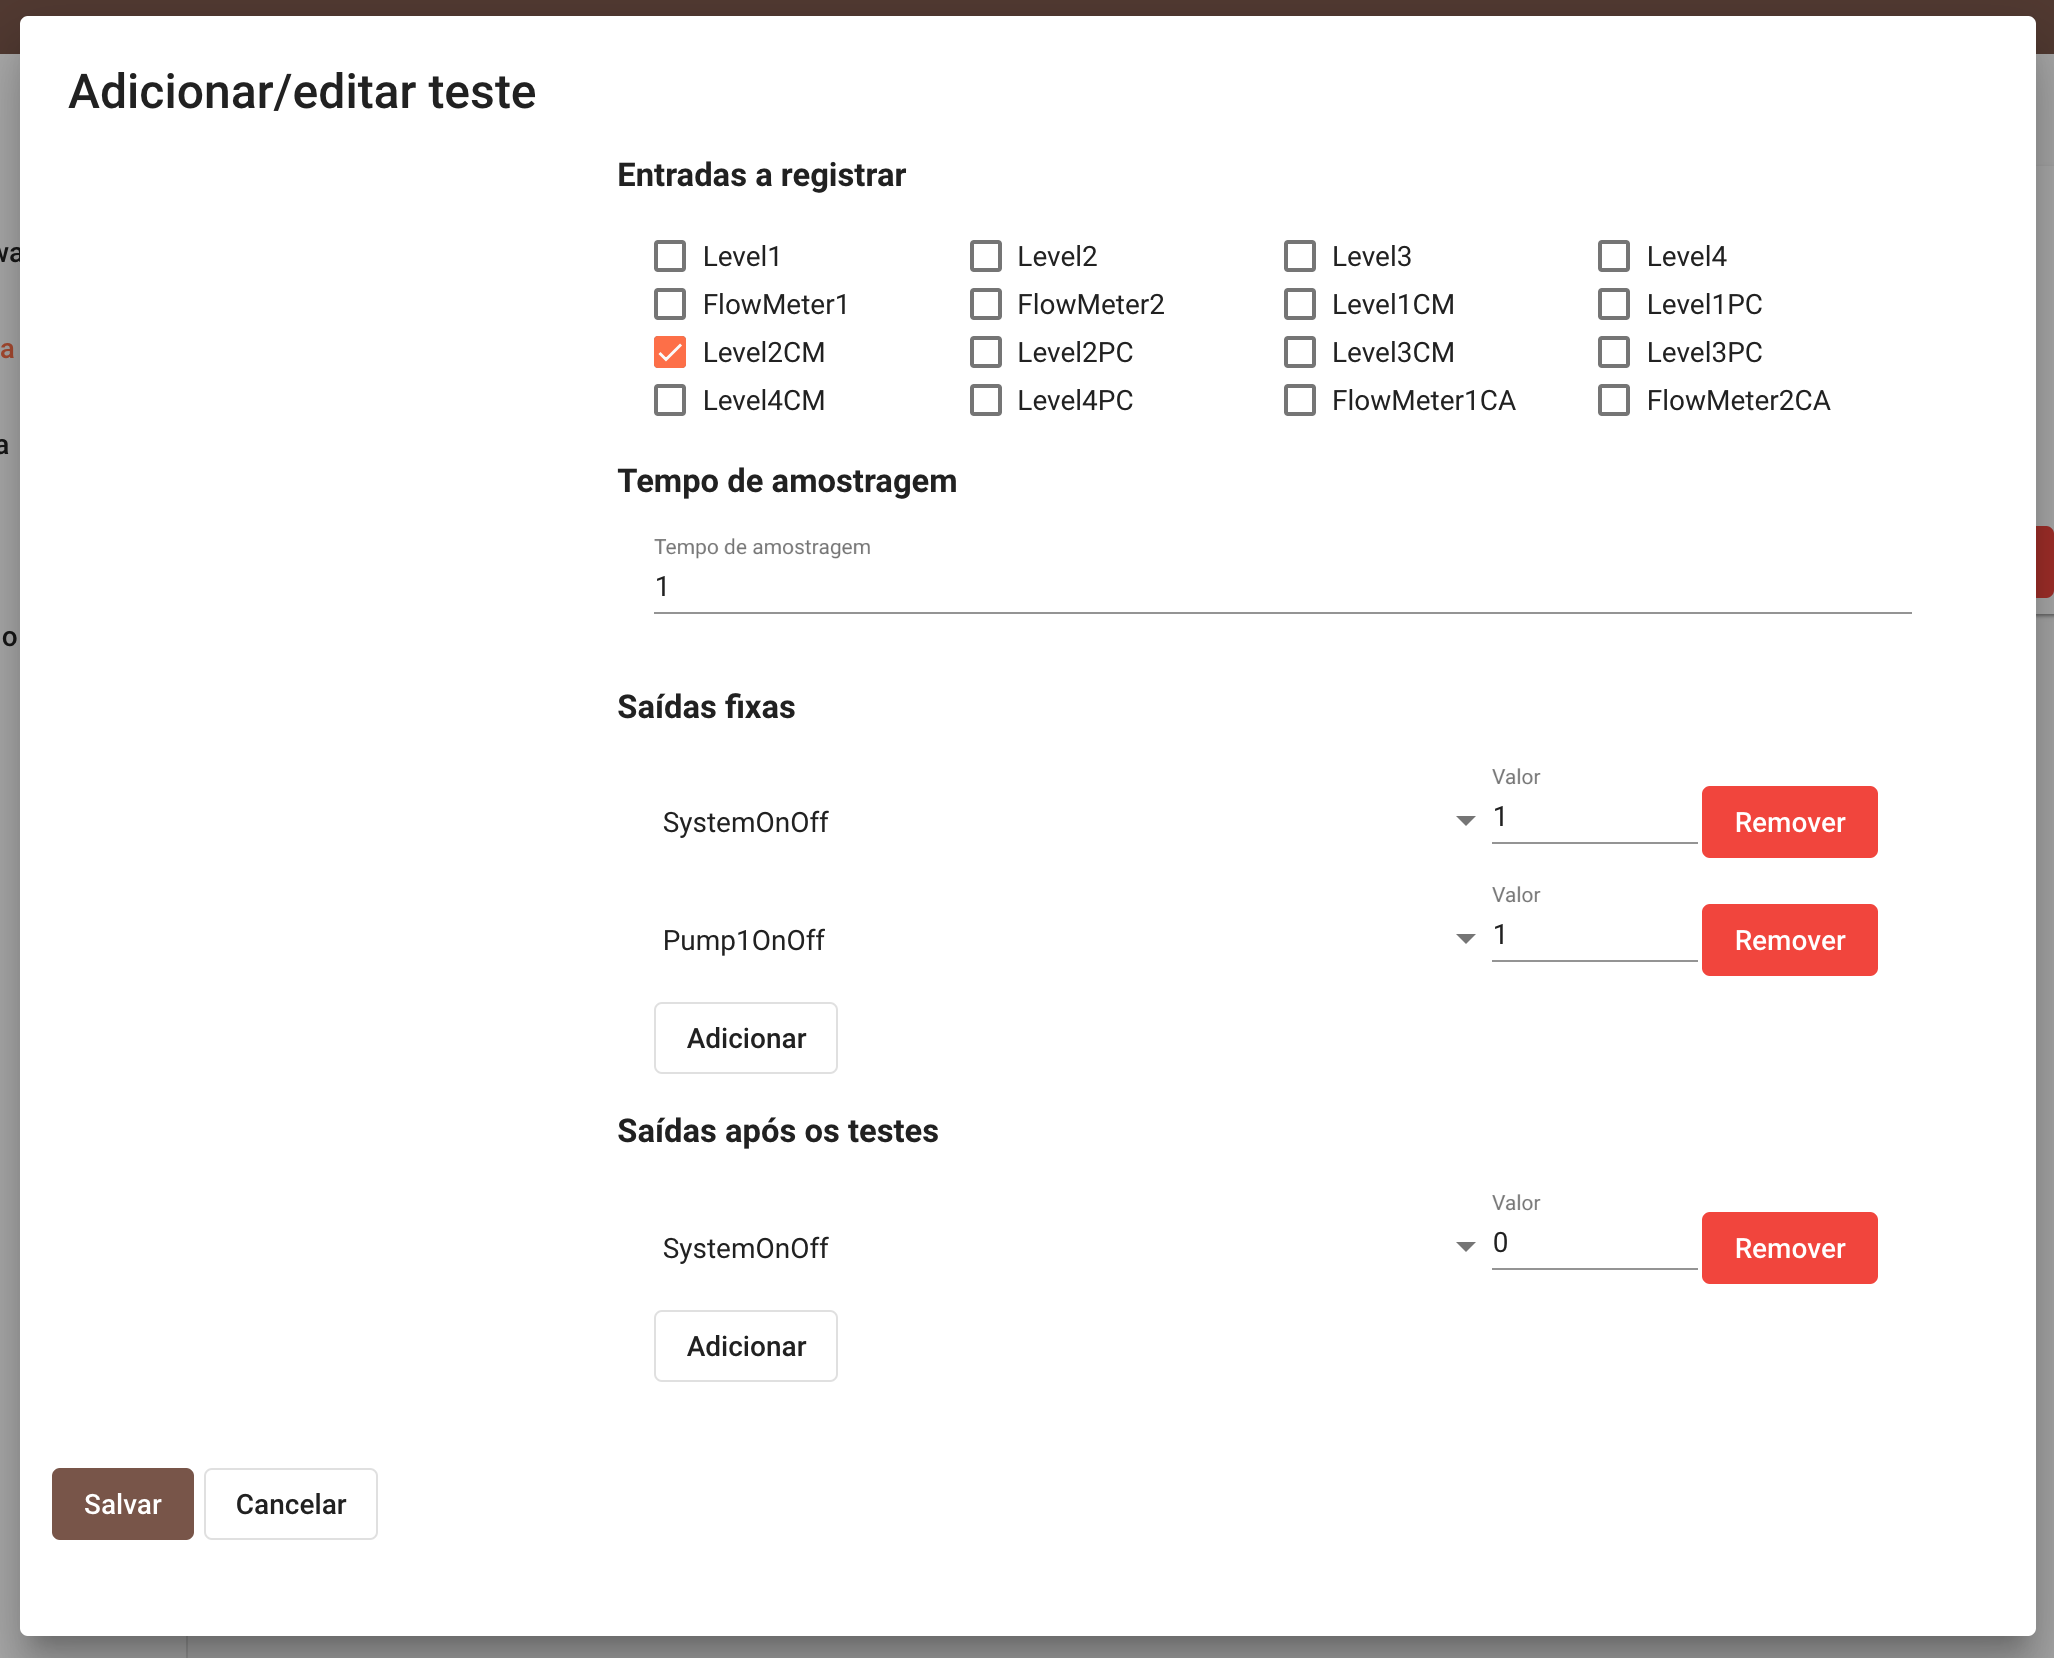
\includegraphics[width=0.9\textwidth]{imgs/system-response3}
    \caption[Configuração comum]{Configuração comum}%
    \label{fig:system-response3}
\end{figure}

\textit{Tempo de amostragem} é o tempo entre cada leitura dos sensores. Os
atuadores também serão atualizados apenas após depassado esse tempo desde a
última atualização.

\textit{Saídas fixas} são portas que terão seus valores escritos antes do teste
iniciar. Seu principal objetivo é permitir definir valores de portas que atuam
como chave geral do sistema. Da mesma forma \textit{Saídas após o teste} serão
definidas após o teste terminar, ou caso algum erro ocorra durante a execução,
como, por exemplo, o acionamento de um intertravamento.

\newpage{}
\section{Impulso}%
\label{sec:impulse}

Nessa aba pode-se definir um sinal do tipo impulso discreto. Deve-se definir as
durações e o valor inicial, mas não a variação da amplitude, como no caso do
sinal degrau. Essa amplitude será calculada de forma a fazer com que o gráfico
do sinal tenha área 1 na região sob \(\Delta{}T\).

\begin{figure}[ht!]
    \centering
    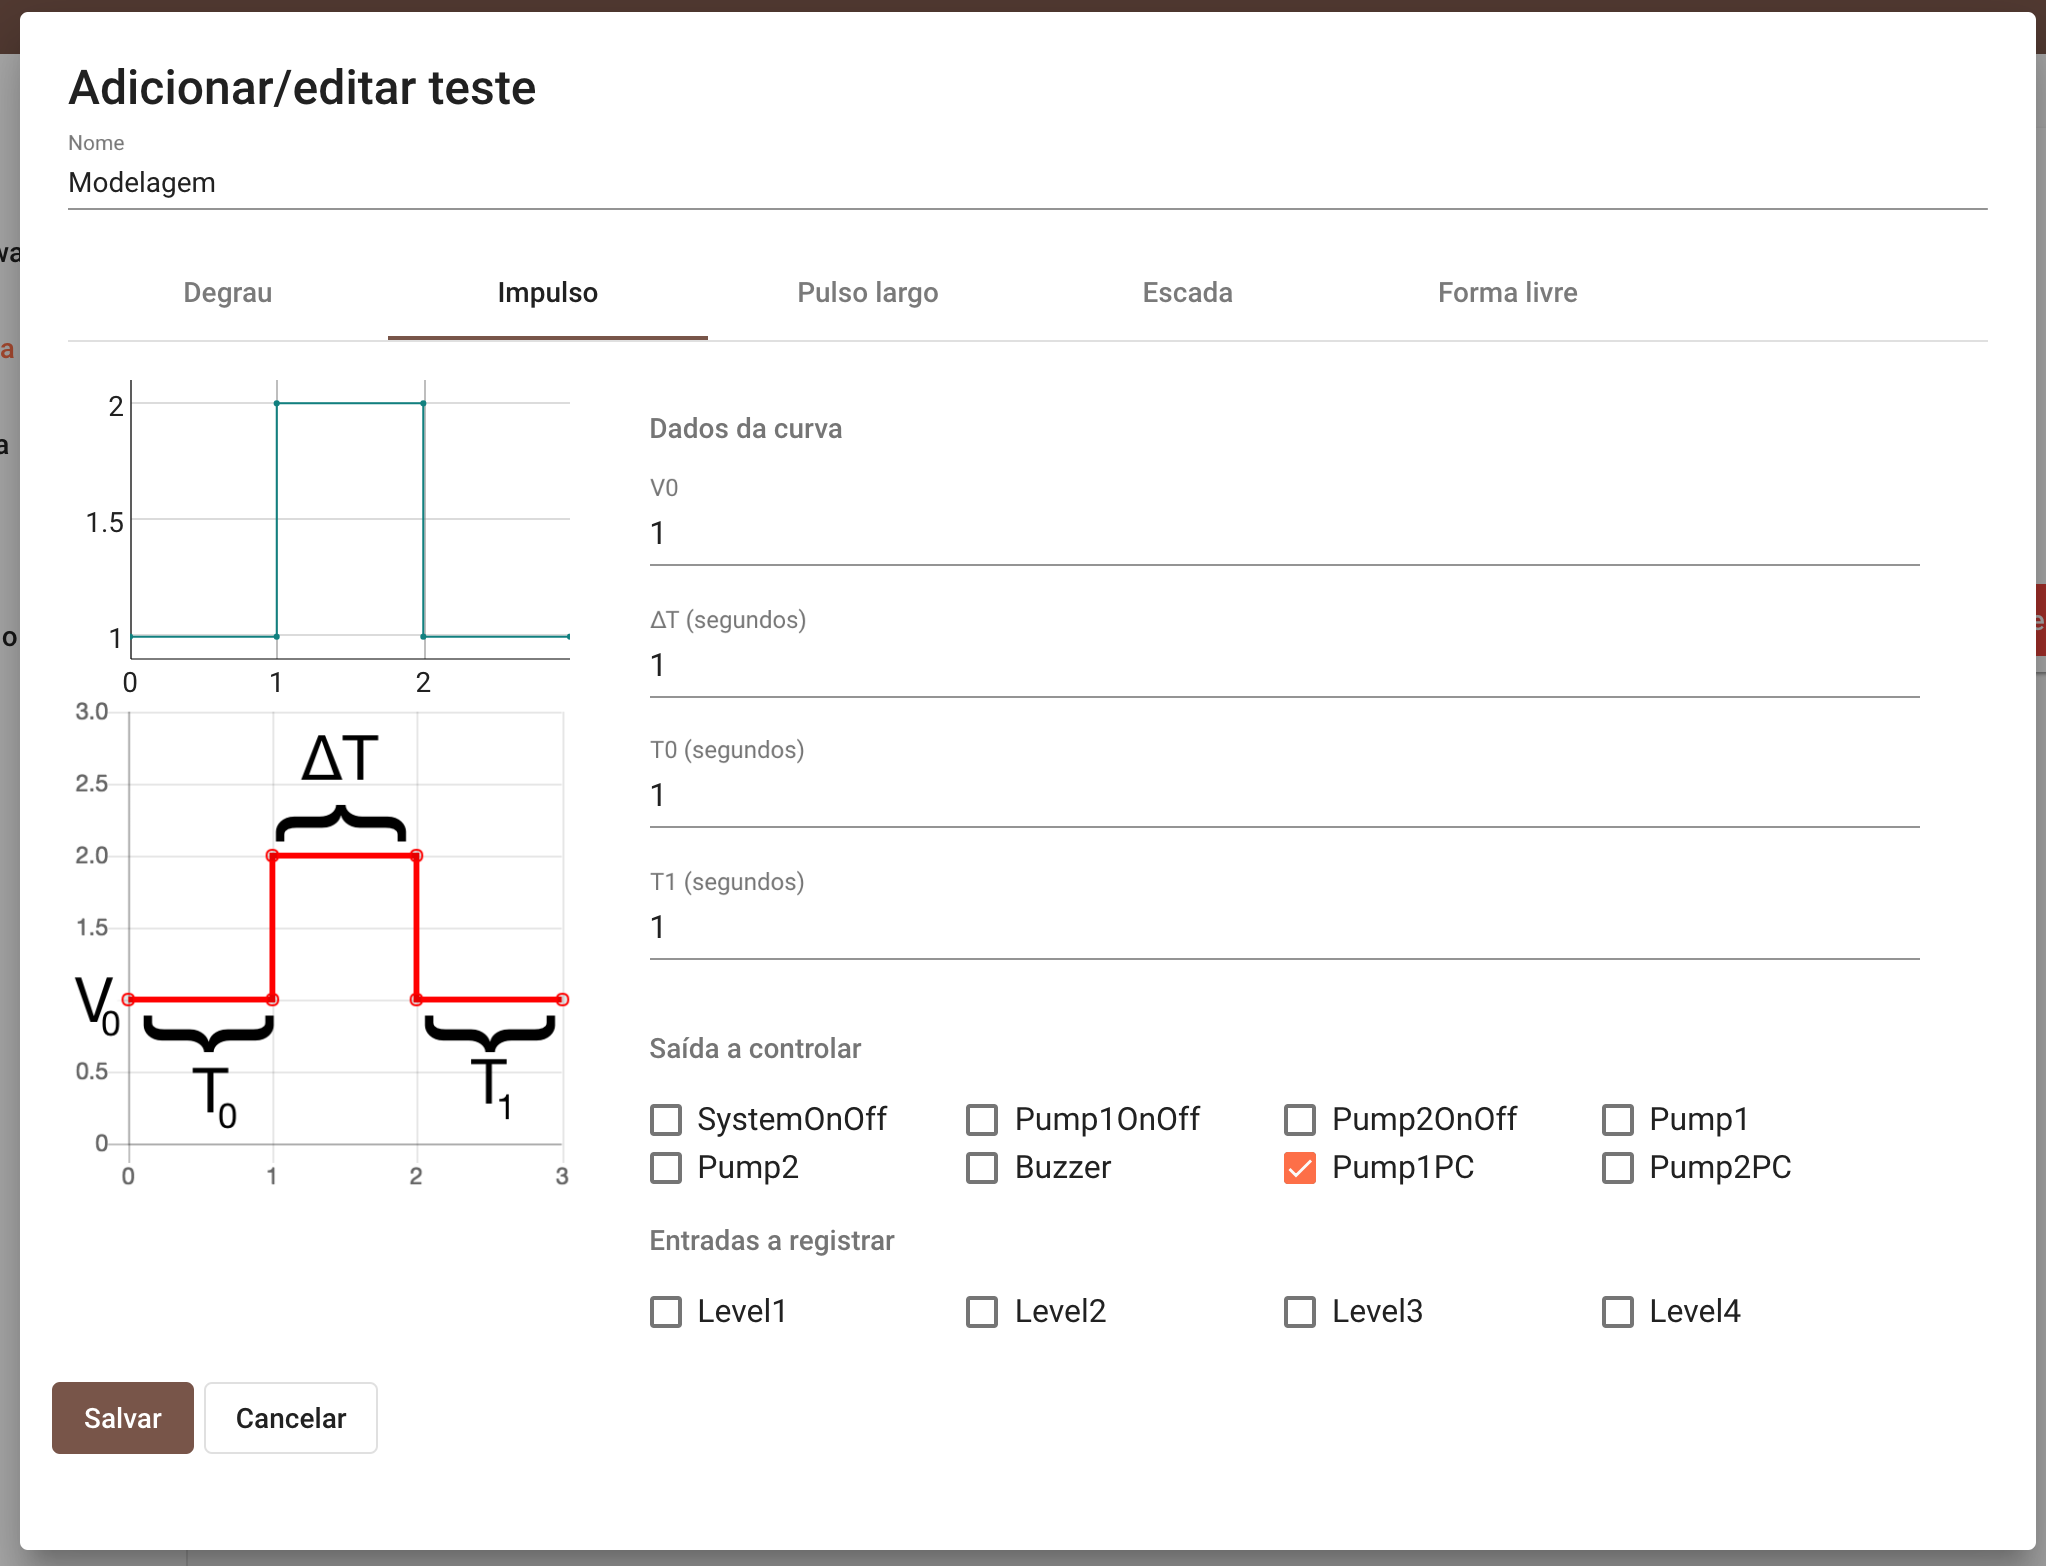
\includegraphics[width=0.9\textwidth]{imgs/system-response4}
    \caption[Impulso]{Impulso}%
    \label{fig:system-response4}
\end{figure}

\newpage{}
\section{Pulso largo}%
\label{sec:wide-pulse}

Parecido com o sinal do tipo degrau, porém deve-se definir um segundo acréscimo
e duração, fazendo com que esse sinal seja a composição de dois sinais do tipo
degrau.

\begin{figure}[ht!]
    \centering
    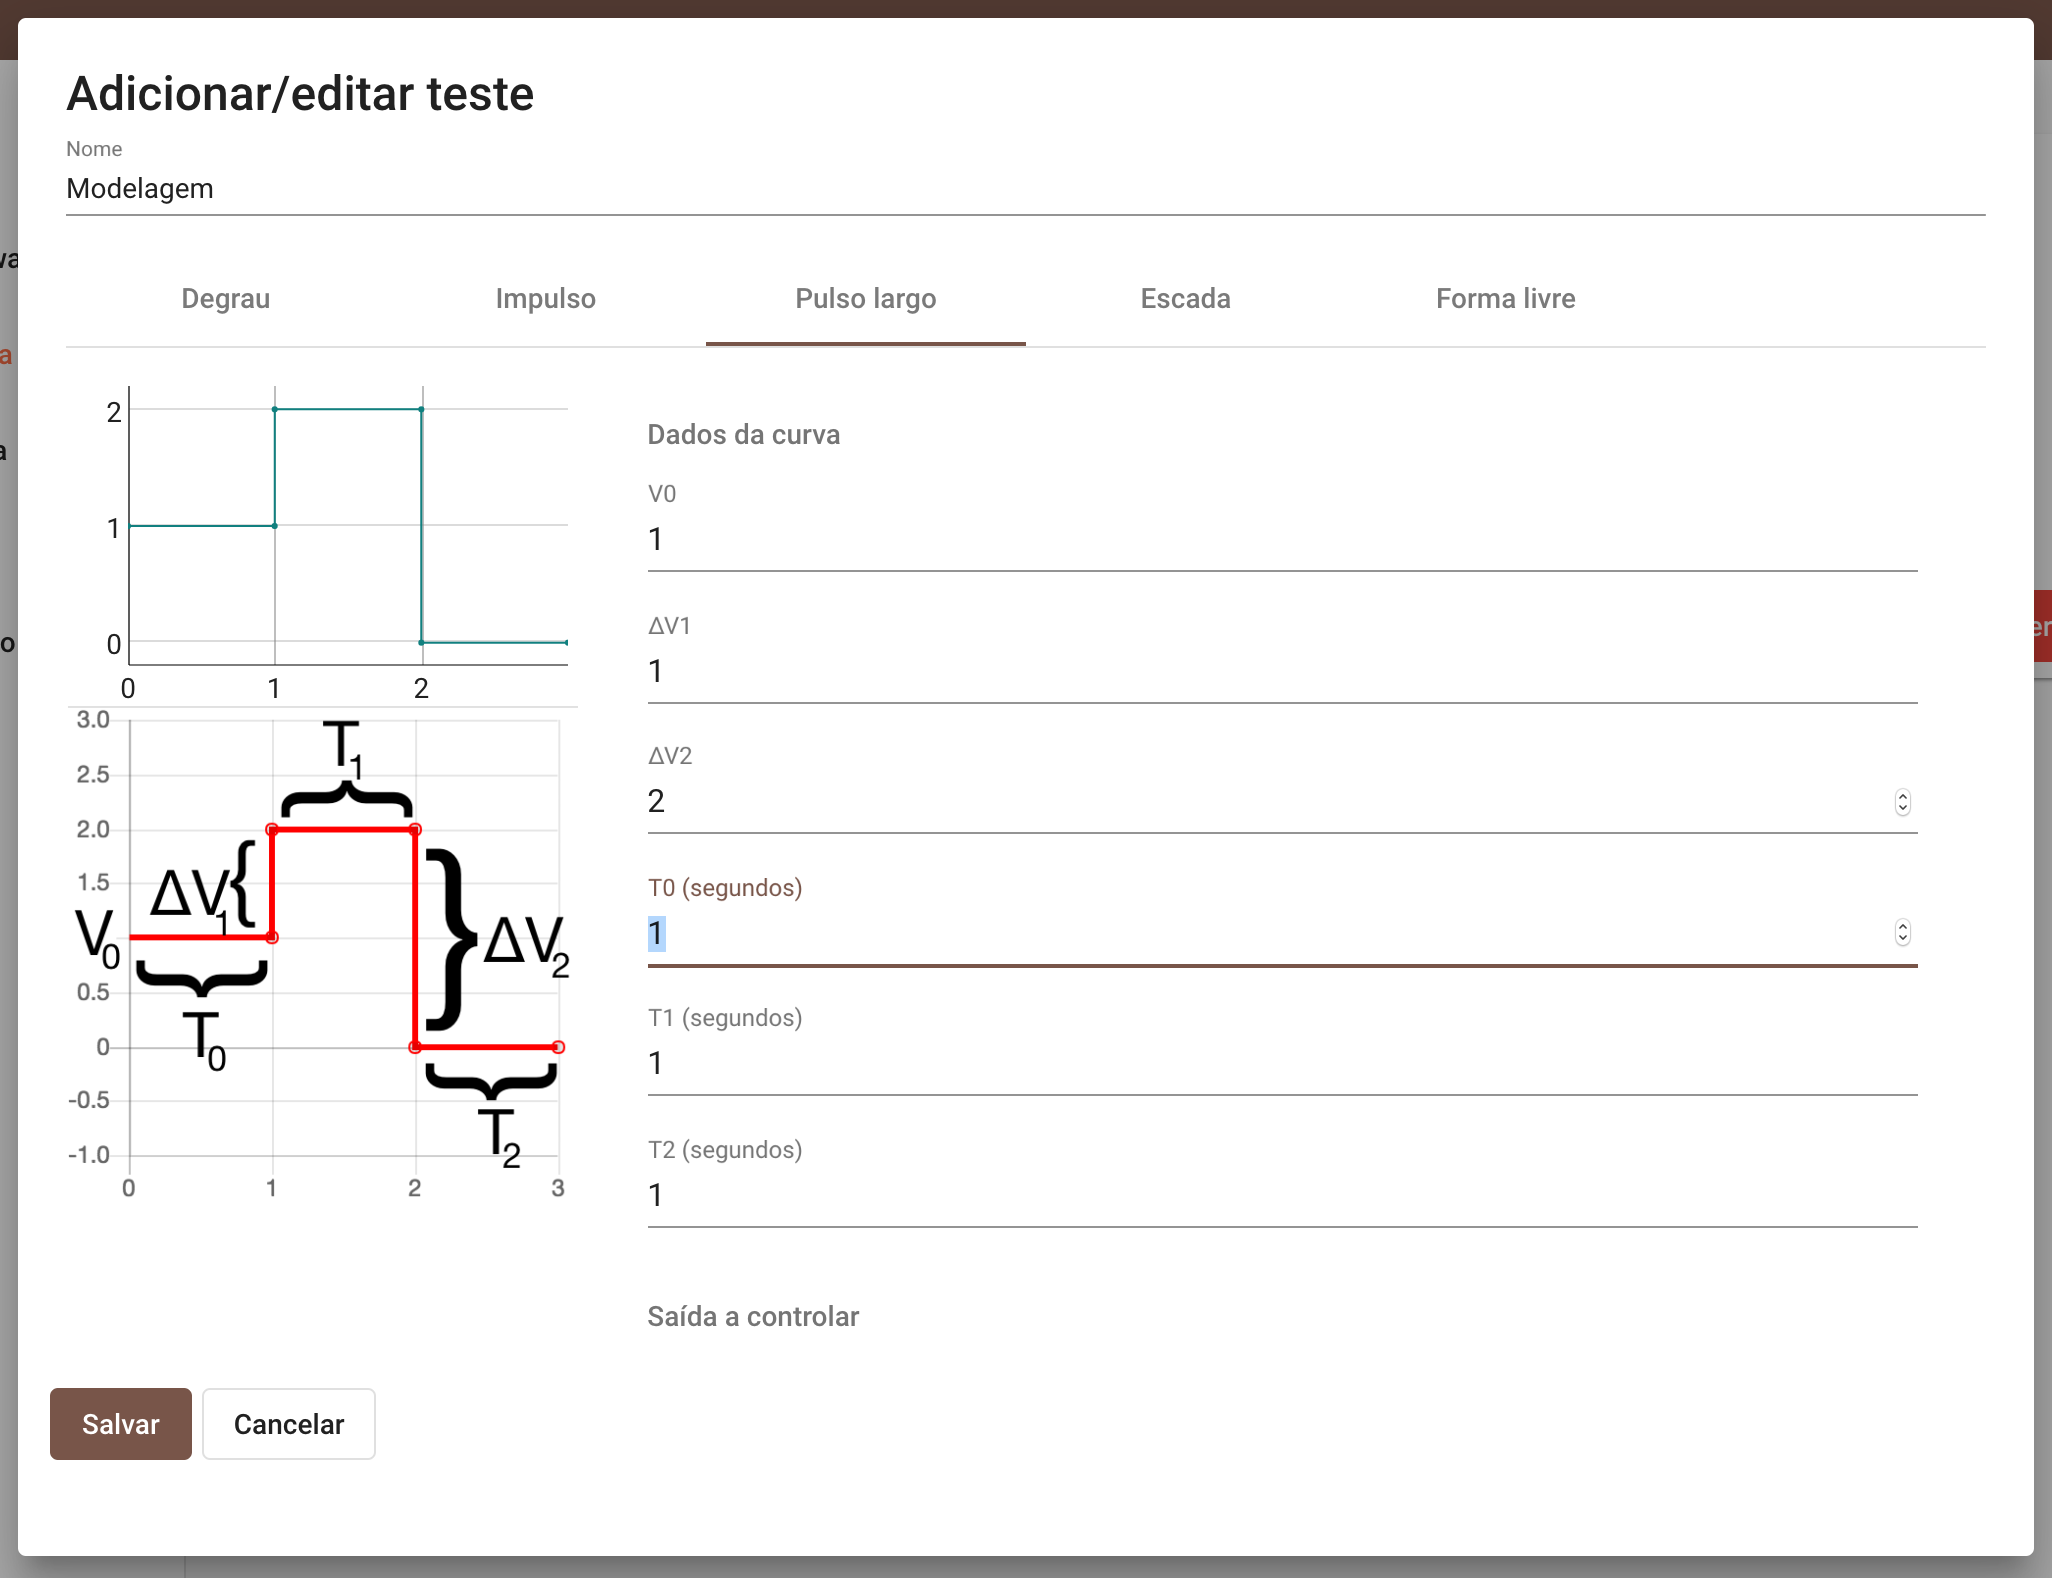
\includegraphics[width=0.9\textwidth]{imgs/system-response5}
    \caption[Pulso largo]{Pulso largo}%
    \label{fig:system-response5}
\end{figure}

\newpage{}
\section{Escada}%
\label{sec:stairs}

Permite a configuração simples de um sinal do tipo escada. Basta informar os
valores incial e final, o número de degraus e a duração de cada degrau.

\begin{figure}[ht!]
    \centering
    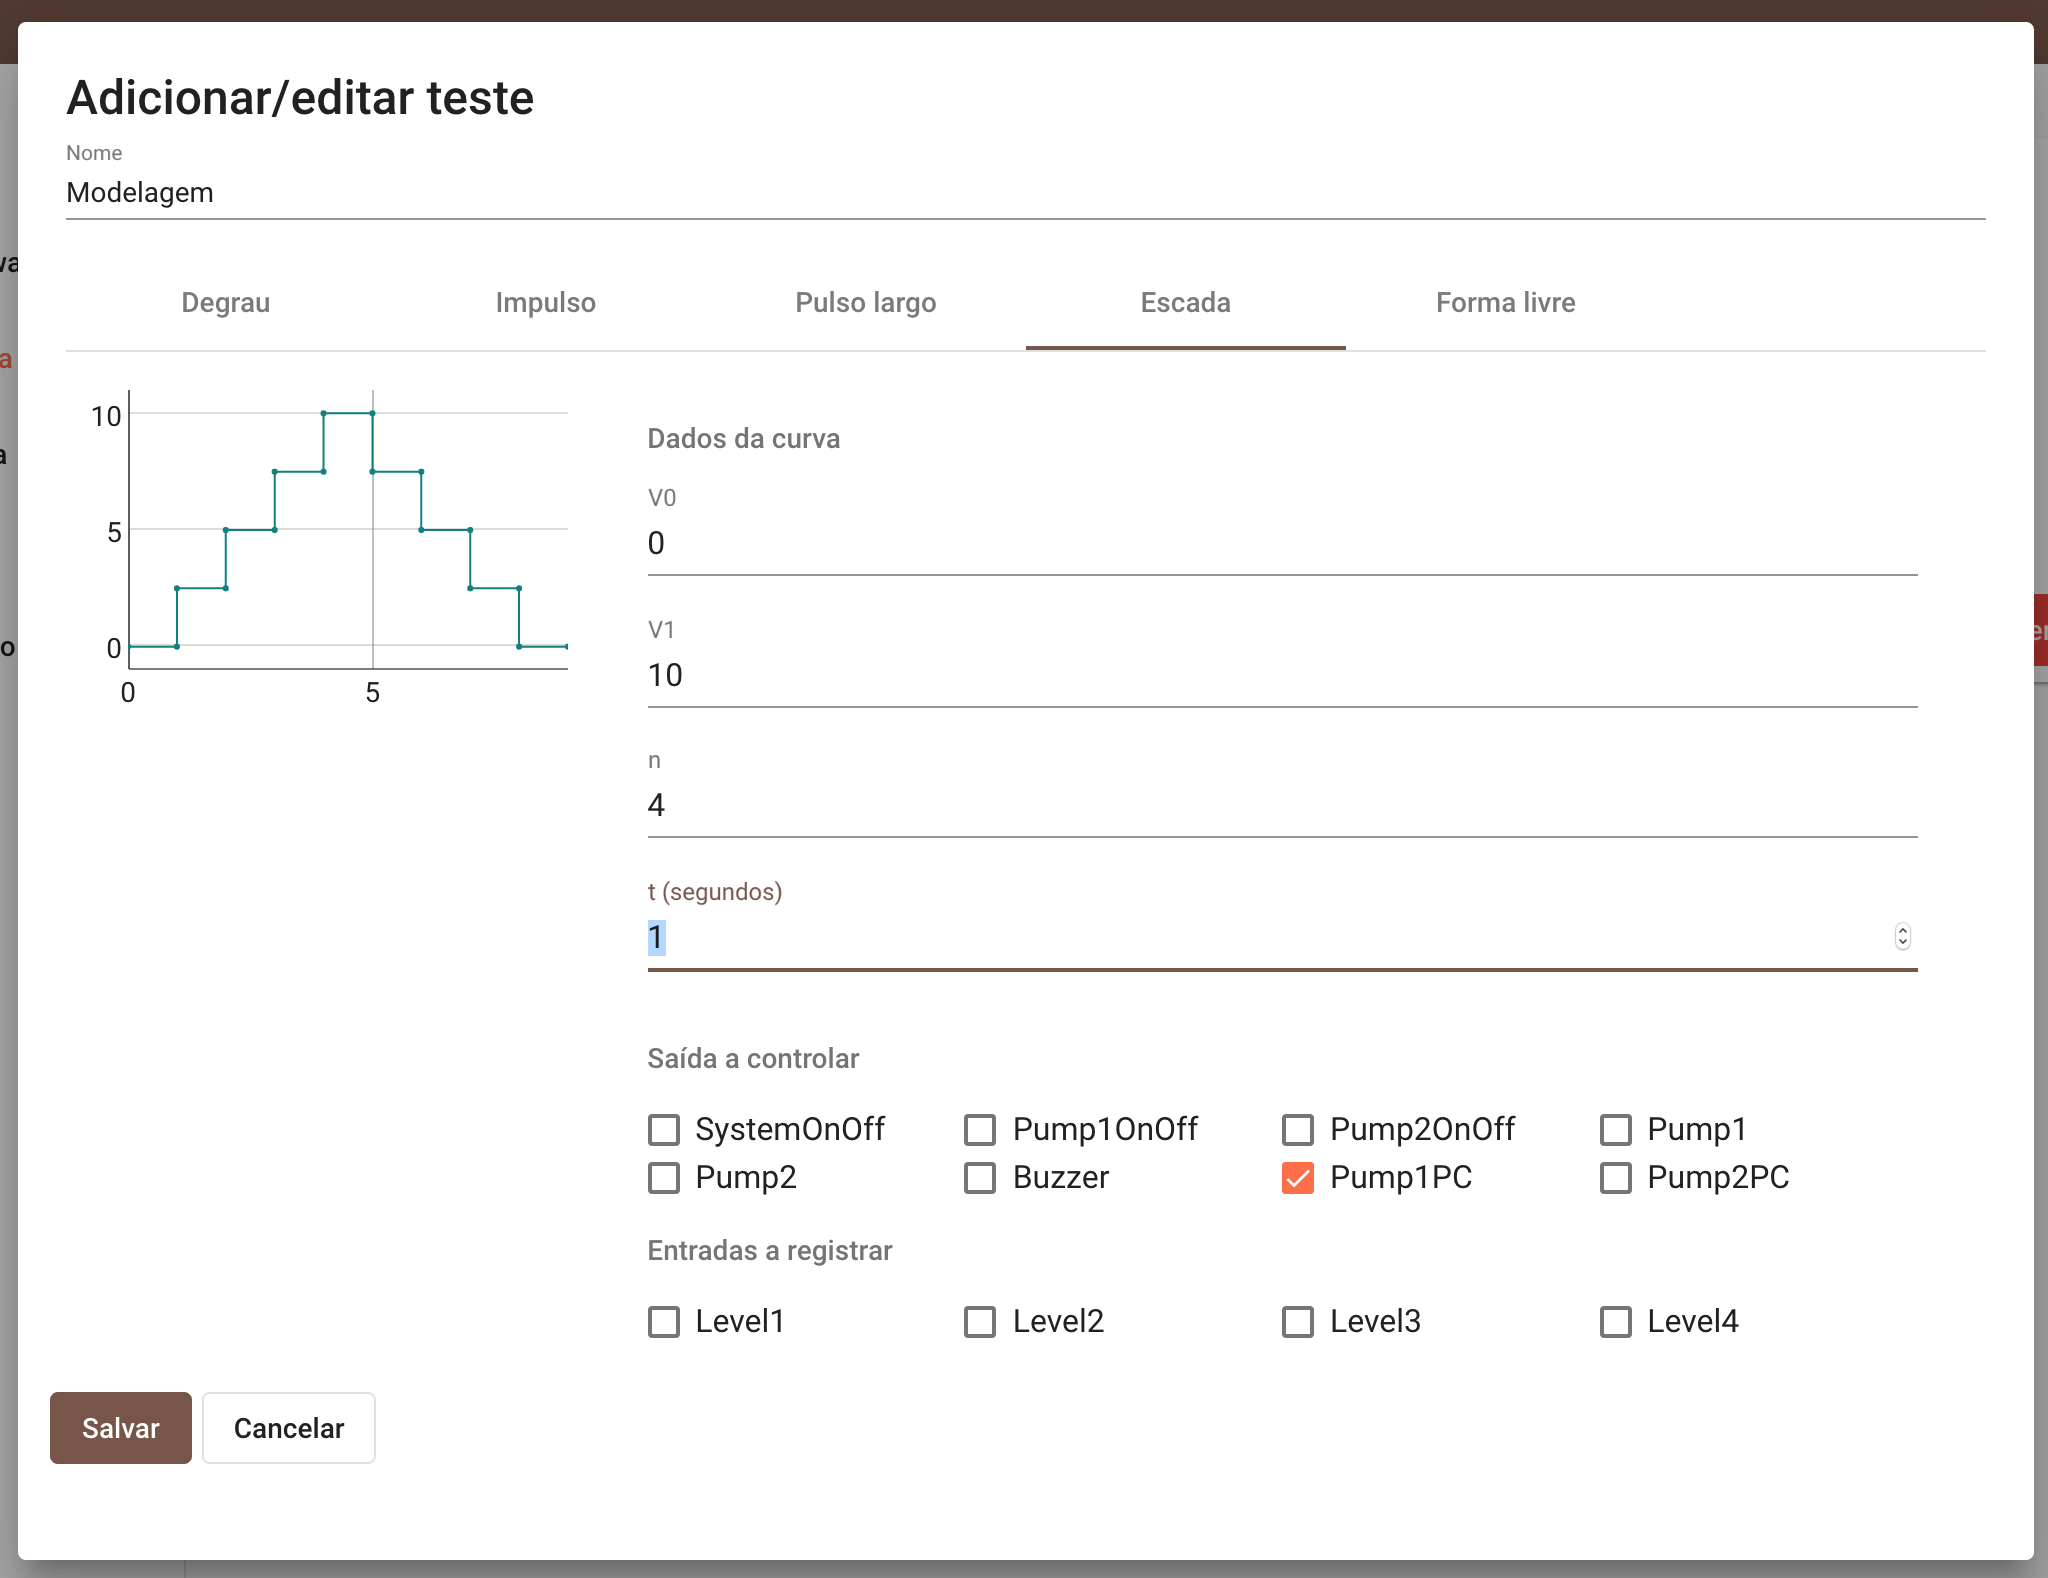
\includegraphics[width=0.9\textwidth]{imgs/system-response6}
    \caption[Escada]{Escada}%
    \label{fig:system-response6}
\end{figure}

\newpage{}
\section{Forma livre}%
\label{sec:free-form}

Nessa aba o sinal pode ser construído ponto a ponto. Também é possível importar
dados de outros aplicativos nos formatos \textit{JSON} e \textit{CSV}. No caso
do \textit{JSON} os dados devem ser no formato \mintinline{javascript}{[{"x": 0,
"y": 0}, {"x": 1, "y": 1}]}. Caso seja usado \textit{CSV}, o tempo deve vir na
primeira coluna e a amplitude na segunda.

O comando \mintinline{matlab}{csvwrite("data.csv", transpose([x; y]))} pode ser
usado para transformar vetores de valores em \textit{CSV}. Após executar esse
comando um arquivo como o nome \textit{data.csv} será criado. Basta abri-lo com
um editor de texto e copiar o conteúdo para a caixa e clicar em
\textit{Importar}.

\begin{figure}[ht!]
    \centering
    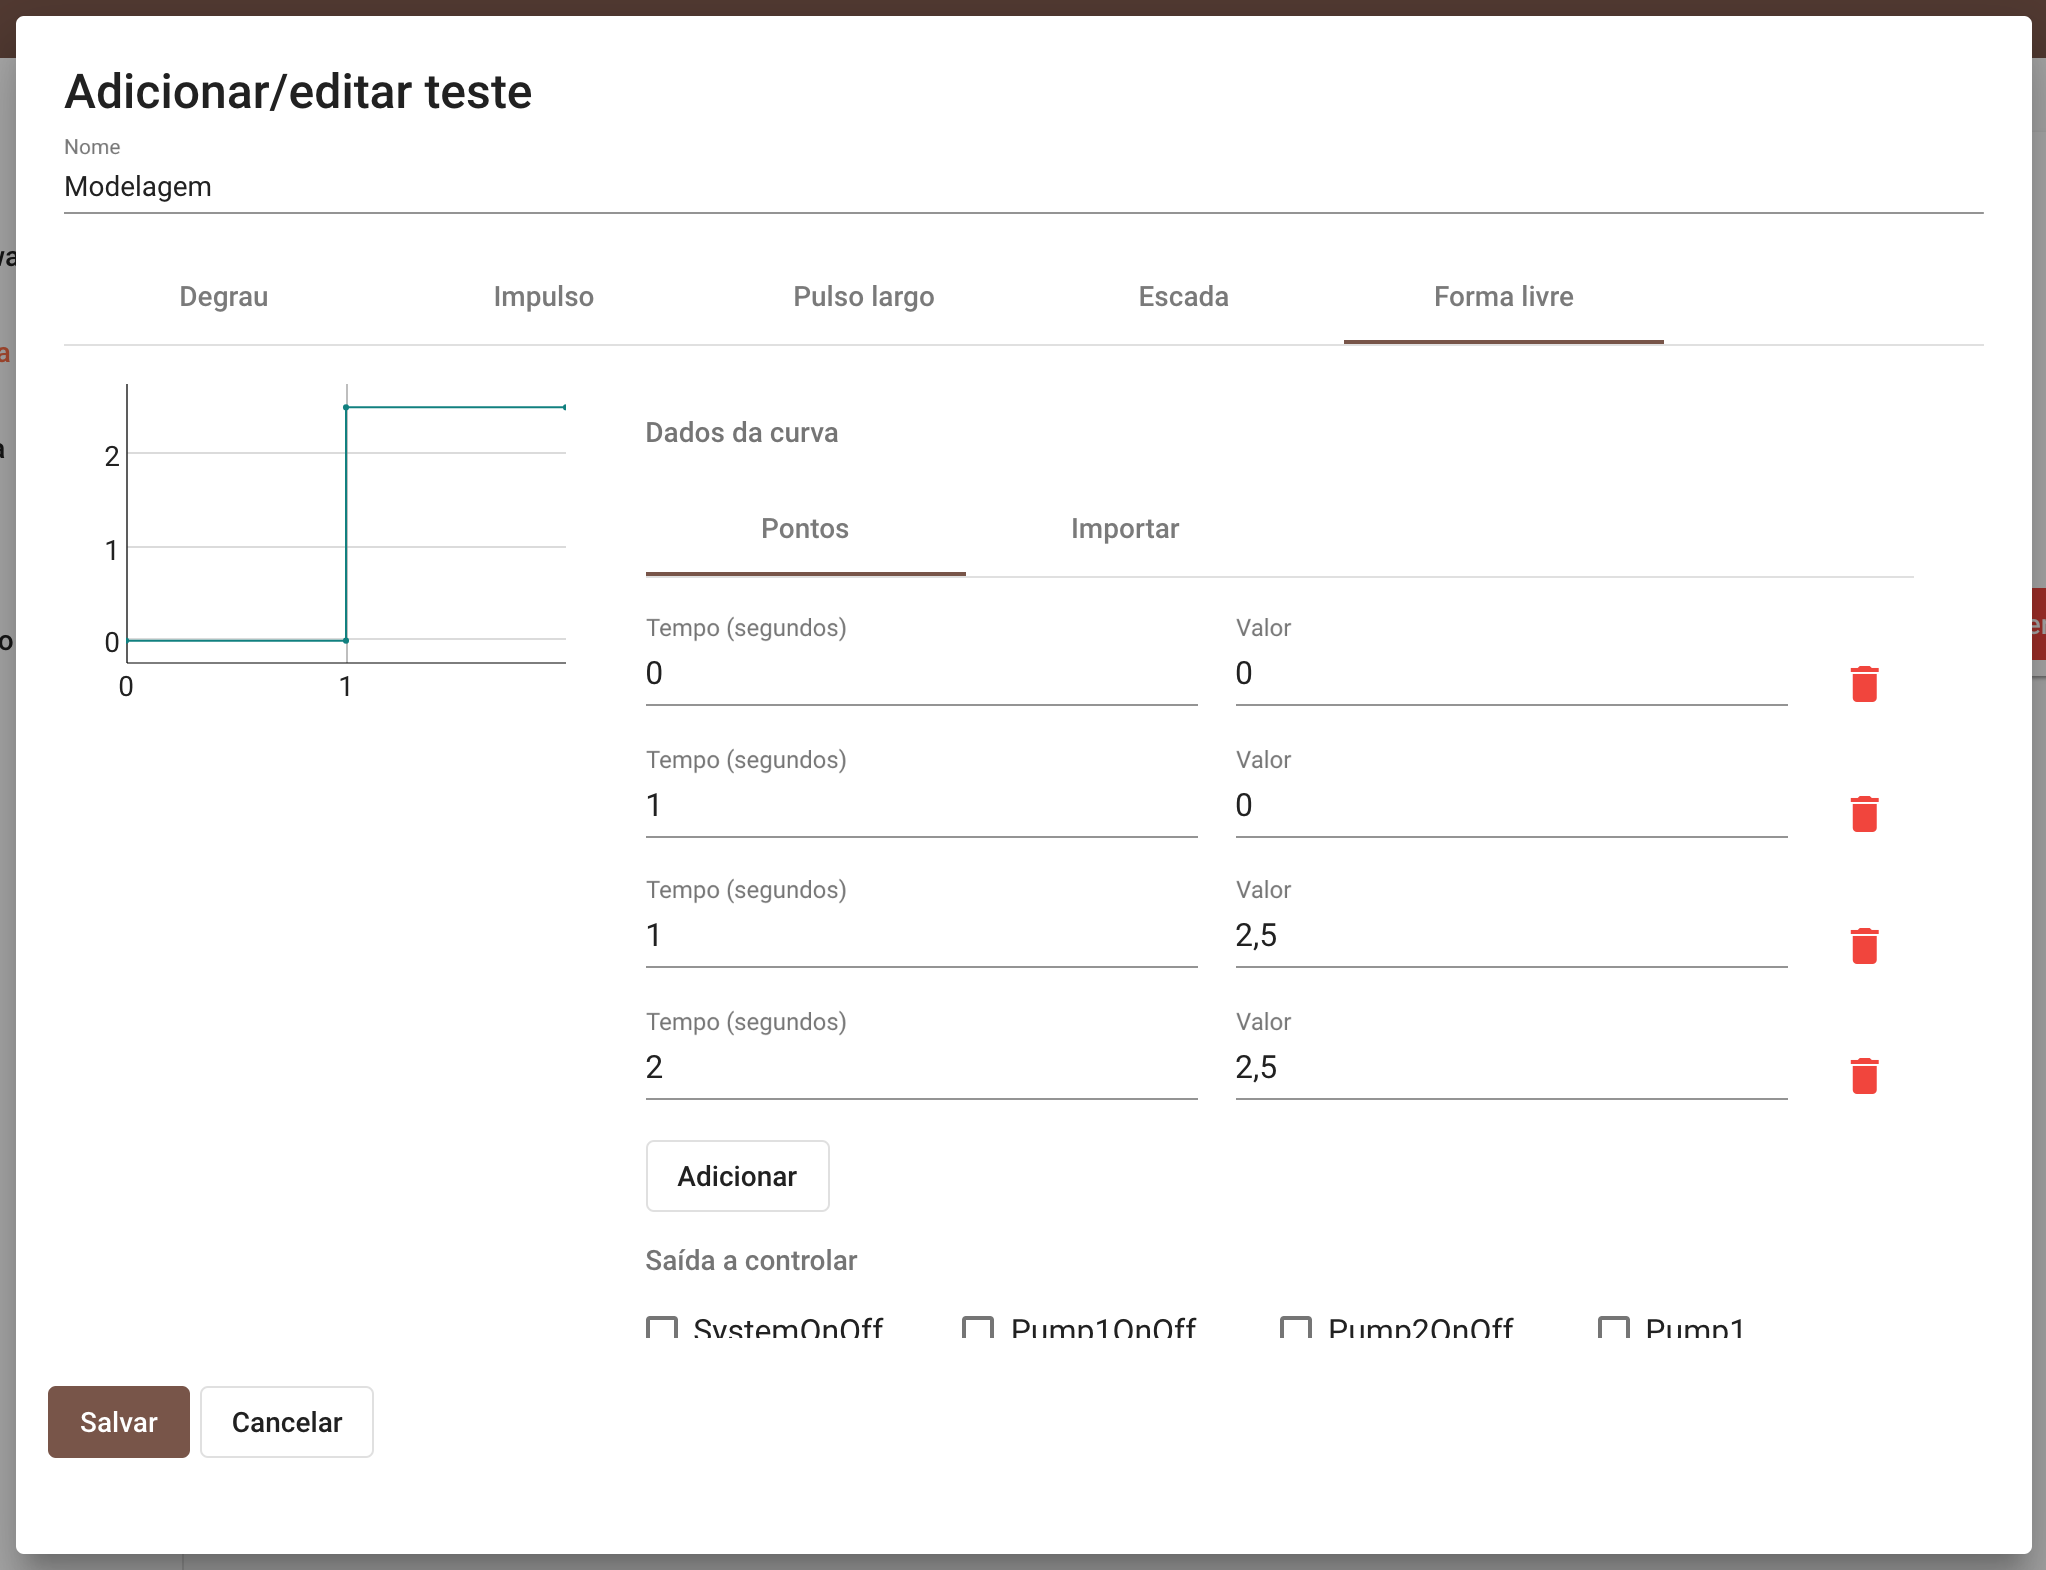
\includegraphics[width=0.9\textwidth]{imgs/system-response7}
    \caption[Forma livre]{Forma livre}%
    \label{fig:system-response7}
\end{figure}

  \cleardoublepage{}
  % !TeX root = document.tex
% !TeX encoding = UTF-8 Unicode

\chapter{Controle do Sistema}%
\label{chapter:system-control}

Esse módulo permite que o usuário escreva testes utilizando a linguagem de
programação \textit{Python}. Dessa forma o usuário tem total liberdade para
controlar as saídas do sistema, e, por dispor de uma linguagem de programação
completa, possibilita o desenvolvimento de qualquer controlador. Embora ideal
para controle em malha fechada, também é útil para criar sinais complexos para a
malha aberta, além de permitir a aplicação de sinais diferentes em portas
diferentes.

A tela inicial do módulo, representada na Figura~\ref{fig:control1}, lista os
controladores salvos. As opções são as mesmas presentes no módulo Resposta do
Sistema (Capítulo~\ref{chapter:system-response}).

\begin{figure}[ht!]
    \centering
    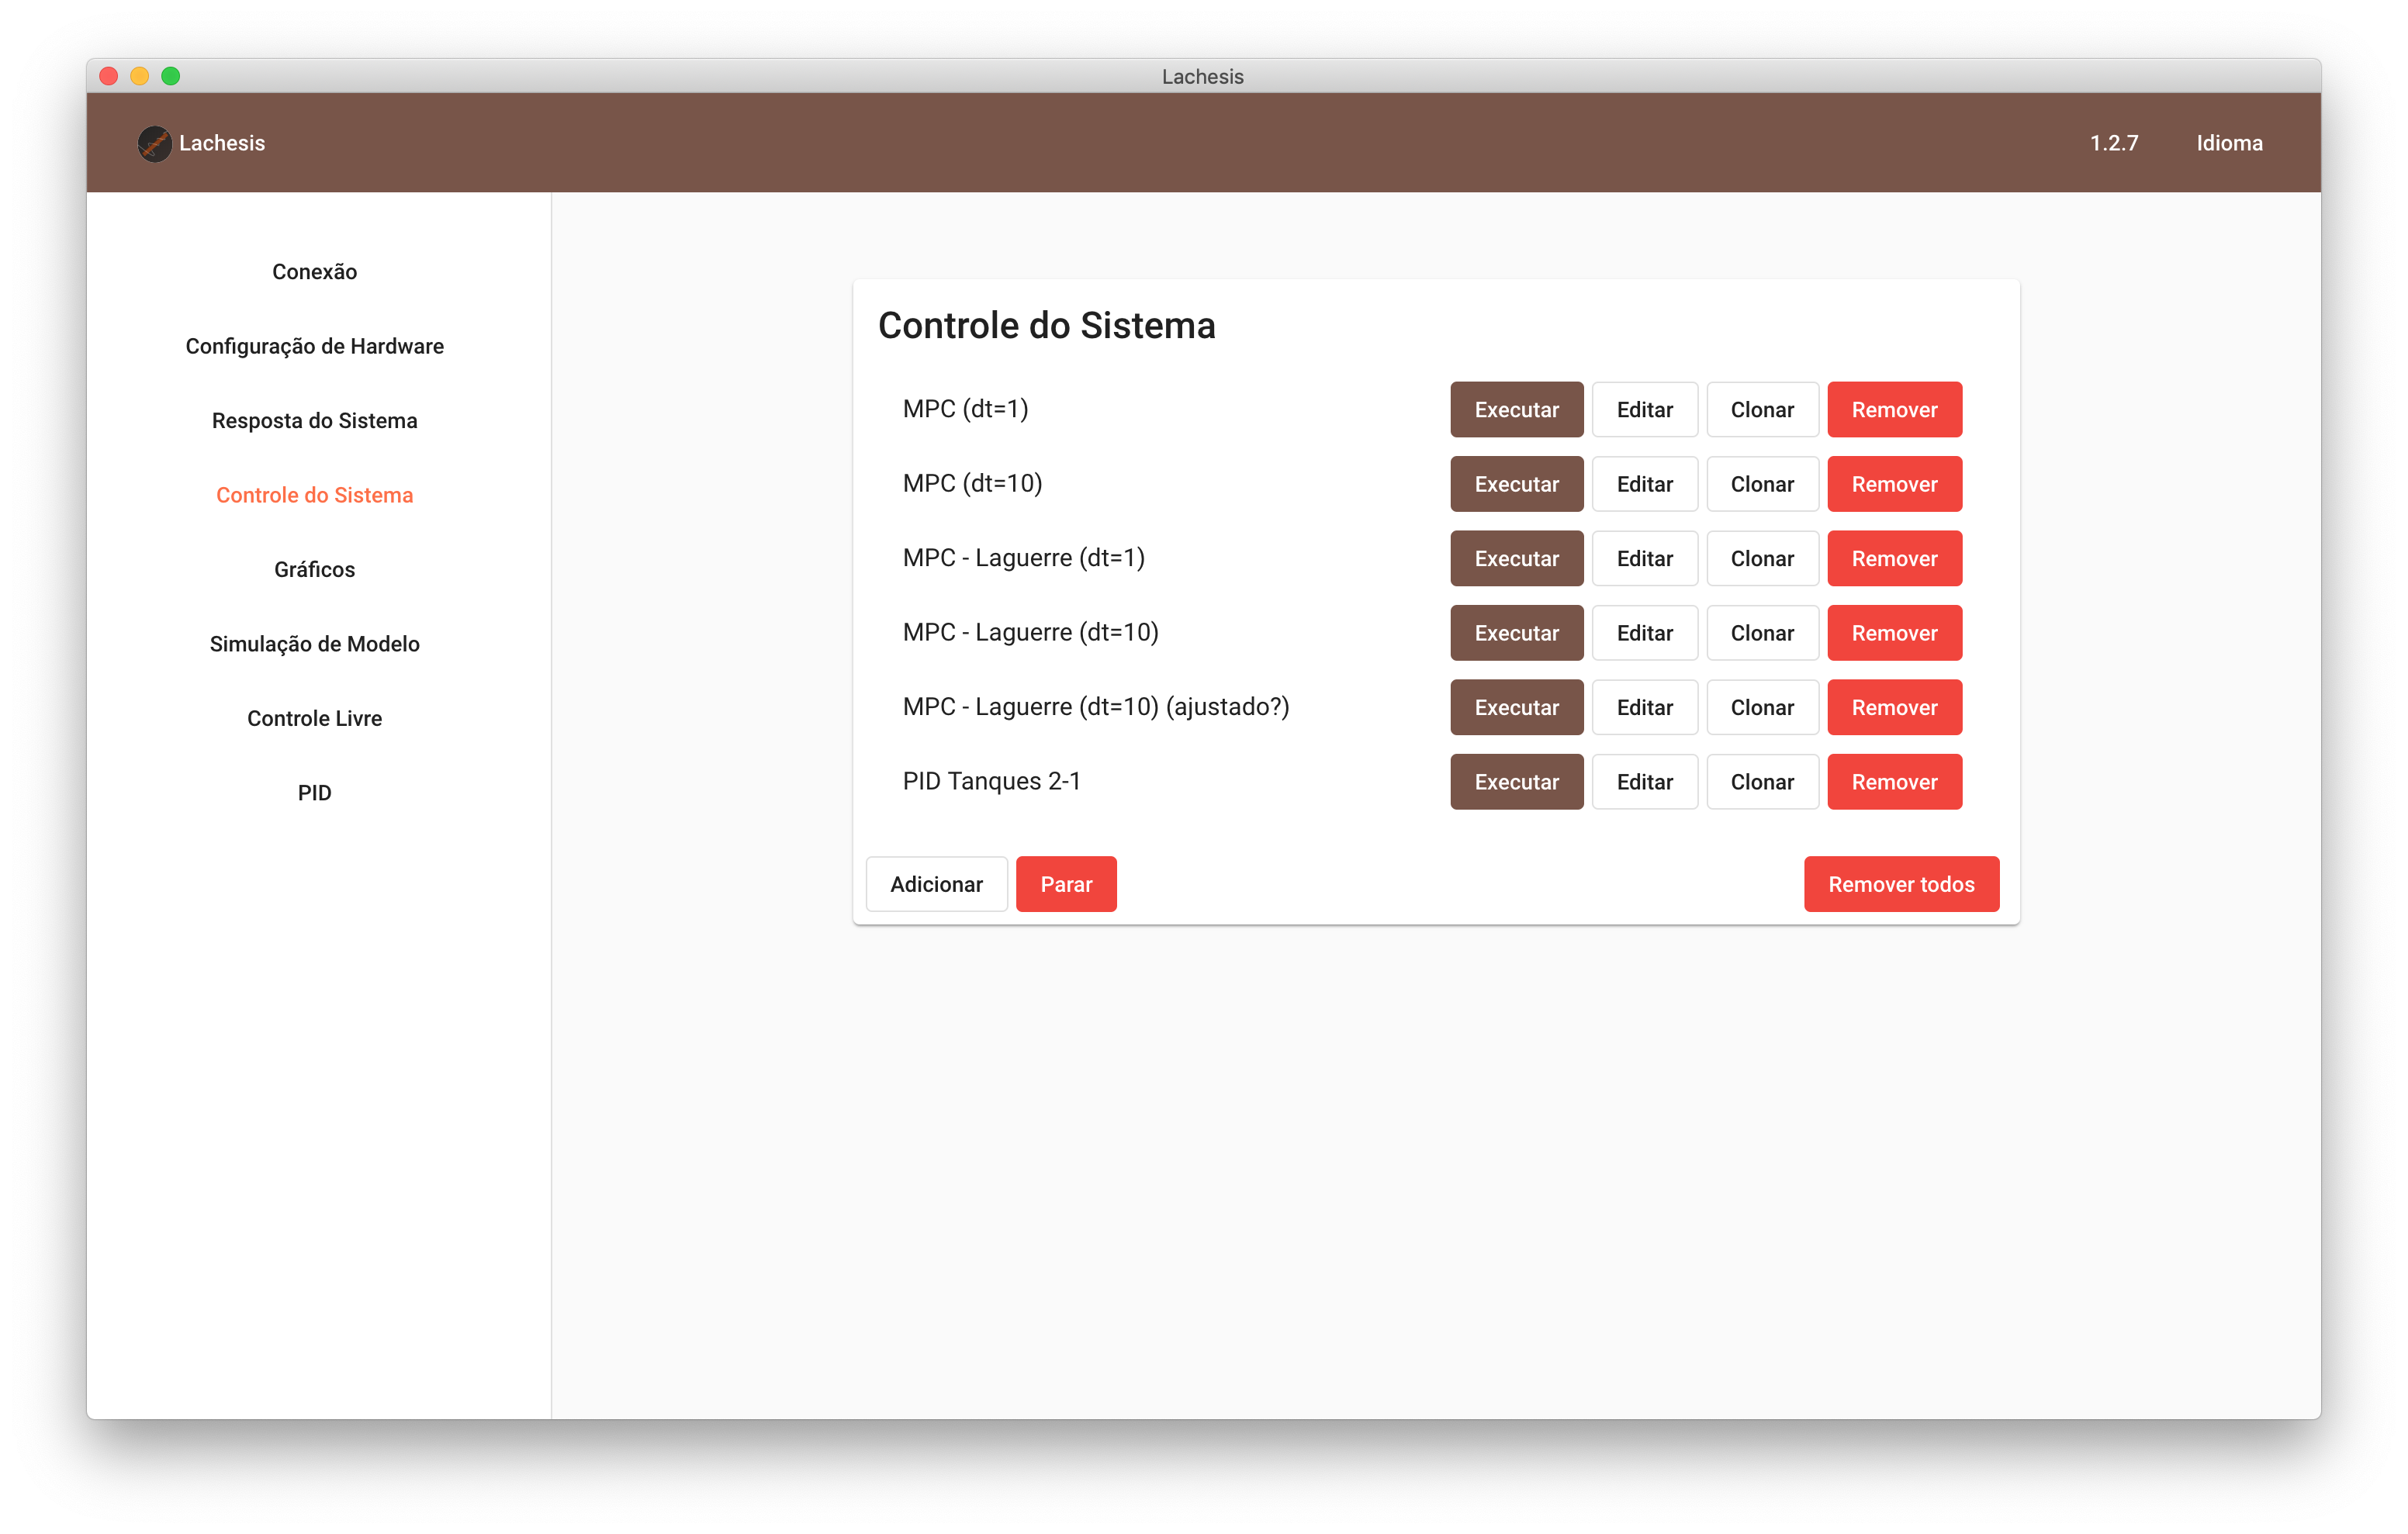
\includegraphics[width=0.9\textwidth]{imgs/control1}
    \caption[Módulo Controle do Sistema]{Módulo Controle do Sistema}%
    \label{fig:control1}
\end{figure}

Ao clicar em \textit{Adicionar} ou em \textit{Editar}, uma nova interface
(Figura~\ref{fig:control2}) se abre permitindo a edição do teste. No topo temos
os campos \textit{Nome}, assim como em \textit{Resposta do Sistema} e sendo
pertinente as mesmas recomendações, \textit{Tempo de amostragem} e \textit{Tempo
total de execução}, que é o tempo máximo que o teste será executado. O mesmo
pode ser interrompido precocemente por motivos de erro ou intertravamento.

\begin{figure}[ht!]
    \centering
    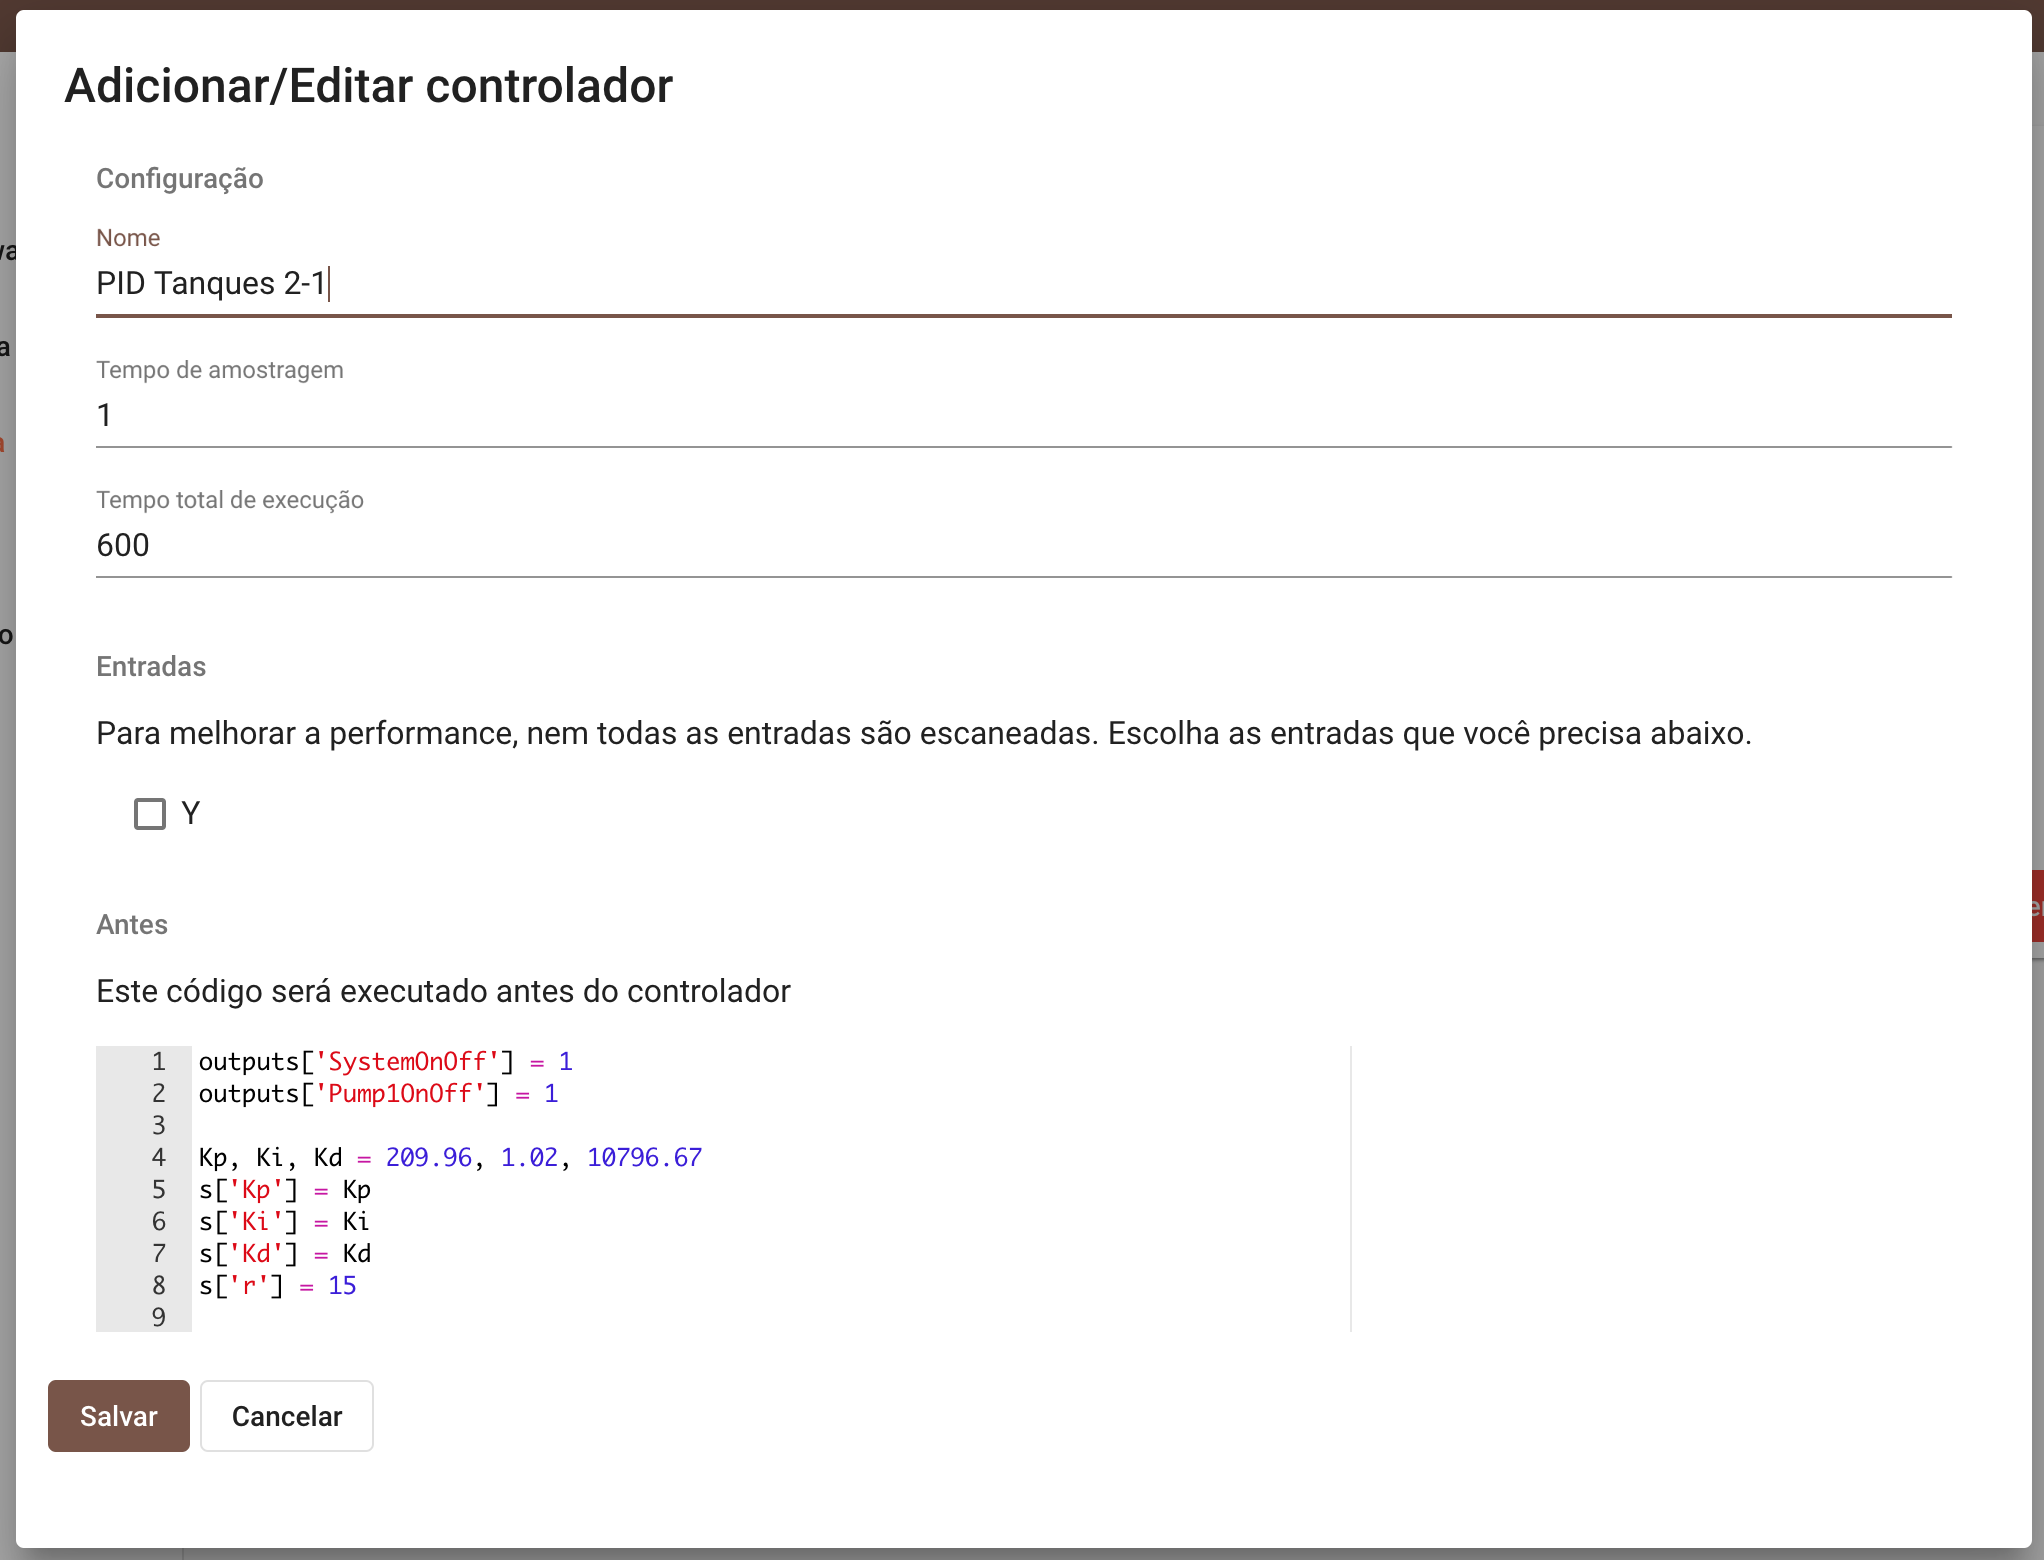
\includegraphics[width=0.9\textwidth]{imgs/control2}
    \caption[Edição de controlador]{Edição de controlador}%
    \label{fig:control2}
\end{figure}

Na seção \textit{Entradas} o usuário deve escolher as portas de entrada que
serão lidas. Apenas as portas selecionadas serão lidas e estarão disponíveis no
código. Isso evita ler informações desnecessárias e agiliza a execução do
código.

No campo \textit{Antes}, visto na Figura~\ref{fig:control3}, podemos inserir o
código que será executado uma vez antes do controlador iniciar. Esse campo é
ideal para calcular ganhos estáticos (como observadores ou \textit{MPC}) e para
salvar informações constantes e valores iniciais, como \(K_p\) ou \(x_0\).

\begin{figure}[ht!]
    \centering
    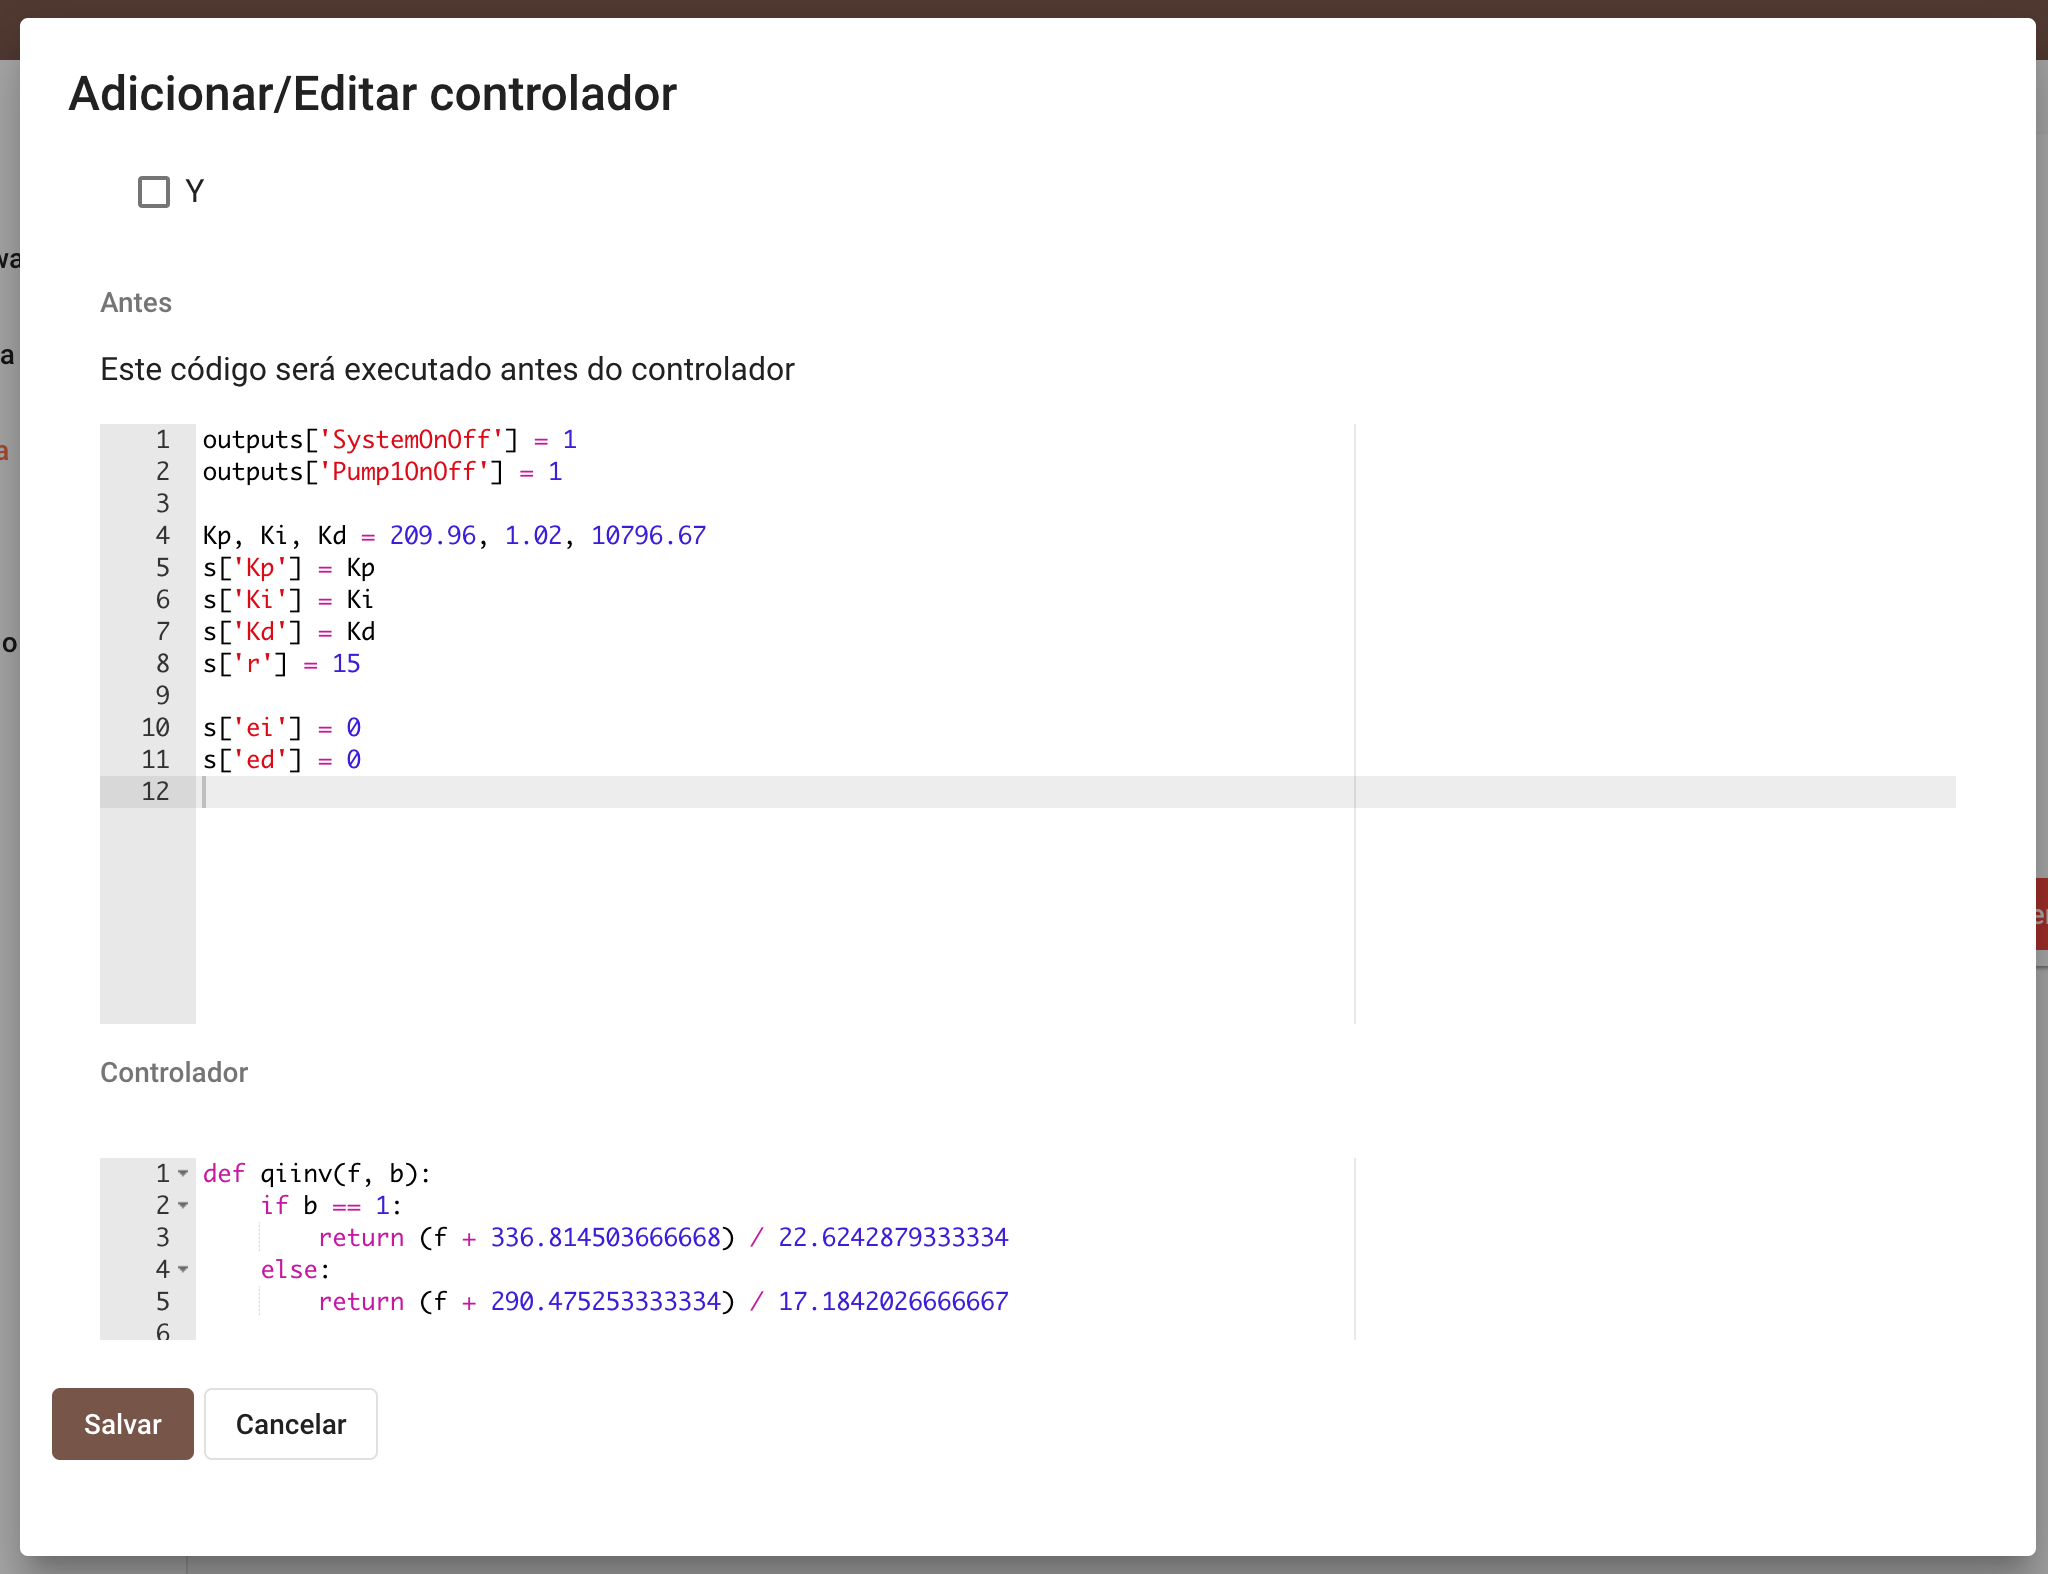
\includegraphics[width=0.9\textwidth]{imgs/control3}
    \caption[Campo \textit{Antes}]{Campo \textit{Antes}}%
    \label{fig:control3}
\end{figure}

Algumas variáveis estão disponíveis nesse campo que o usuário pode fazer uso:

\begin{itemize}
    \item \textbf{inputs} um dicionário com o valor lido na entrada logo antes
                          da execução desse campo. Na Figura~\ref{fig:control2}
                          podemos ver que a entrada \textit{S9} foi selecionada,
                          logo podemos ler seu valor acessando
                          \mintinline{python}{inputs['S9']}.
    \item \textbf{outputs} um dicionário inicialmente vazio. Ao fim da execução
                           desse bloco todas as saídas que forem adicionadas a
                           esse dicionário serão aplicadas no \textit{hardware}.
                           Por exemplo, para ligar a bomba 1 de um sistema,
                           configrada em \textit{Configurações de Hardware} como
                           \textit{Pump1PC} com 40\% de potência, podemos
                           utilizar o código
                           \mintinline{python}{outputs['Pump1PC'] = 40}.
    \item \textbf{s} variável de estado. Essa variável é um dicionário e estará
                     disponível na próxima seção. Ela deve ser usada para
                     persistir dados durante a execução do teste. Por exemplo, o
                     estado atual de um modelo em espaço de estados pode ser
                     salvo nessa variável e alterado posteriormente durante a
                     execução do controlador. É como se fosse uma variável
                     global. Exemplo de uso: \mintinline{python}{s['Kp'] = 1}.
    \item \textbf{dt} o tempo de amostragem.
    \item \textbf{np} a biblioteca numpy já é importada e está disponível sob o
                      nome \textit{np}, não sendo necessário reimportá-la.
    \item \textbf{math} a biblioteca math já é importada, não sendo necessário
                        reimportá-la.
\end{itemize}

No campo \textit{Controlador} (Figura~\ref{fig:control4}) deve-se inserir o
código que será executado a cada \textit{tempo de amostragem} segundos. As
mesmas variáveis disponíveis no campo \textit{Antes} estão disponíveis nesse
campo, além de:

\begin{itemize}
    \item \textbf{t} tempo de execução em segundos.
    \item \textbf{log} todas as entradas e saídas nas variáveis \textbf{inputs}
                       e \textbf{outputs} são salvas e podem ser vistas em
                       gráficos e exportadas para arquivos. A variável
                       \textbf{log} permite fazer a mesma coisa com variáveis
                       que não são entrada ou saída. Por exemplo, pode-se gerar
                       uma entrada para o erro na saída adicionando o erro a
                       esse dicionário, assumindo que o valor da saída anterior
                       esteja salvo como \textit{y\_anterior}:
                       \mintinline{python}{log['erro'] = y - s['y_anterior']}.
                       Na seção \textit{Gráficos}
                       (Capítulo~\ref{chapter:graficos}) a variável
                       \textit{erro} estará disponível nas opções de variáveis
                       de gráficos e de exportação de dados.
\end{itemize}

\begin{figure}[ht!]
    \centering
    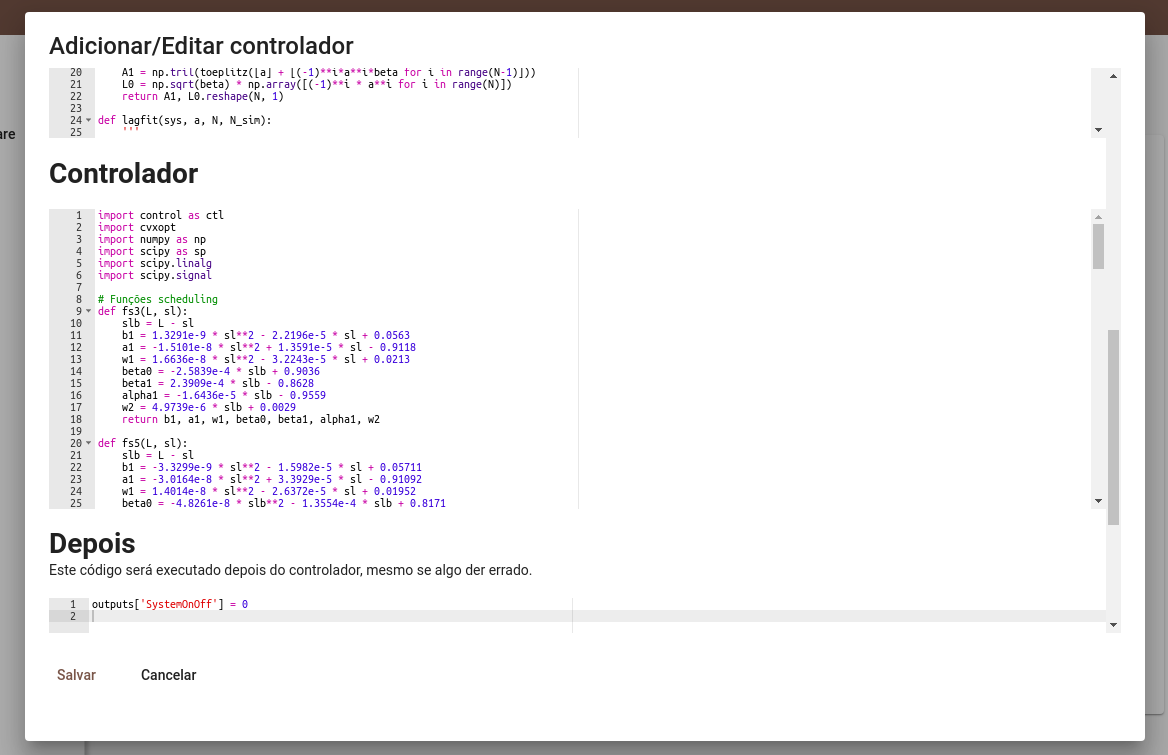
\includegraphics[width=0.9\textwidth]{imgs/control4}
    \caption[Campo \textit{Controlador}]{Campo \textit{Controlador}}%
    \label{fig:control4}
\end{figure}

No campo \textit{Depois} (Figura~\ref{fig:control5}) pode-se inserir código para
desligar o sistema. Esse campo será executado em caso de erro ou caso o teste
execute até o final. Apenas a variável \textit{outputs} está disponível nesse
campo.

\begin{figure}[ht!]
    \centering
    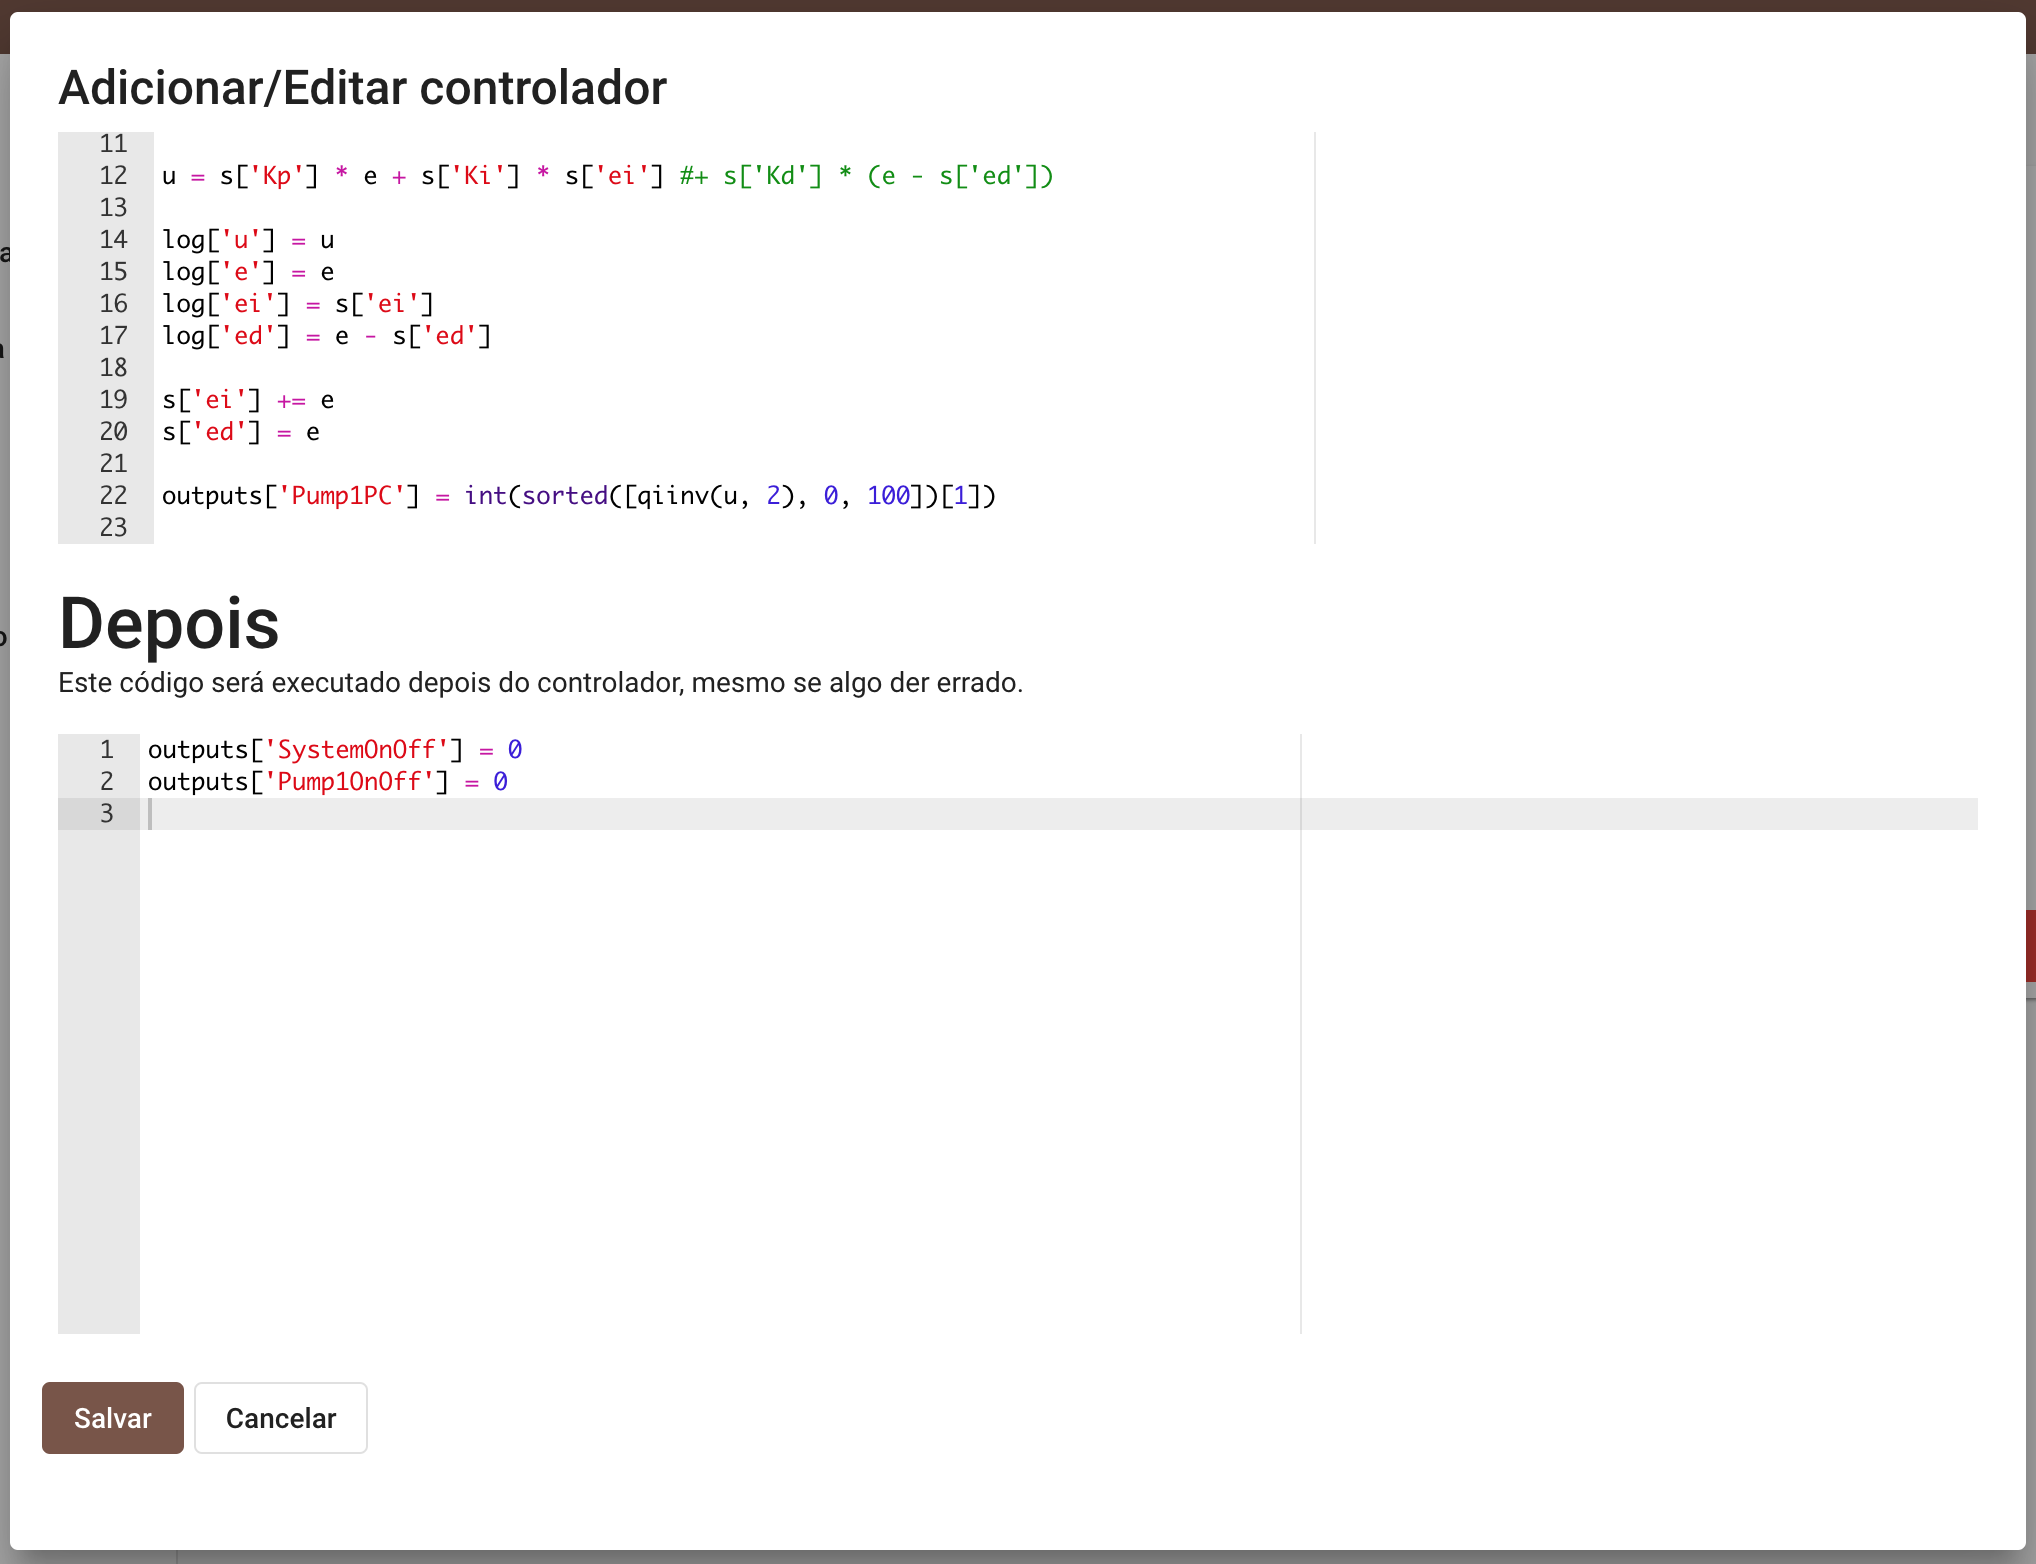
\includegraphics[width=0.9\textwidth]{imgs/control5}
    \caption[Campo \textit{Depois}]{Campo \textit{Depois}}%
    \label{fig:control5}
\end{figure}

O pseudo-código abaixo representa o funcionamento do programa, como se os campos
fossem funções. Obviamente a implementação real é bem mais complexa. Deve-se
chamar atenção ao fato que o controlador será executado sempre num tempo
múltiplo de \textit{dt}. O cálculo do tempo de espera leva em conta o tempo que
foi necessário para executar o código, e sempre aguardará para iniciar a próxima
execução em um múltiplo. Se o tempo de execução do código for menor que
\textit{dt}, então o código sempre executará em \textit{k*dt} segundos. Se o
código levar mais de \textit{dt} segundos para executar, a próxima execução será
agendada para o próximo \textit{k*dt}.

\newpage{}
\begin{pythoncode}
    import math
    import numpy as np

    s = dict()
    outpus = dict()
    inputs = moirai.read_inputs()
    dt = moirai.test_dt()

    s, outputs = user.antes(inputs, outpus, s, dt, math, np)
    
    moirai.write_outputs(outputs)
    
    while True:
        t = moirai.sleep(dt)
        inputs = moirai.read_inputs()
        log = dict()
        outputs = dict()
        
        s, outputs, log = user.controlador(inputs, s, dt, math, np, t, log)

        moirai.write_outputs(outputs)
        moirai.save_variables(inputs, outputs, log)
    
    outpus = dict()
    outputs = user.depois(outputs)
    moirai.write_outputs(outputs)
\end{pythoncode}

  \cleardoublepage{}
  % !TeX root = document.tex
% !TeX encoding = UTF-8 Unicode

\chapter{Gráficos}%
\label{chapter:graficos}

Esse módulo exibe os gráficos dos testes realizados e do teste em execução. Nele
é possível visualizar os sinais em tempo real durante a execução do teste. Nos
testes finalizados é possível exportar os dados. Na Figura~\ref{fig:graphs1}
podemos ver a listagem de gráficos com as opções pertinentes. O botão
\textit{Parar} funciona como nos módulos \textit{Resposta do Sistema} e
\textit{Controle do Sistema}.

\begin{figure}[ht!]
    \centering
    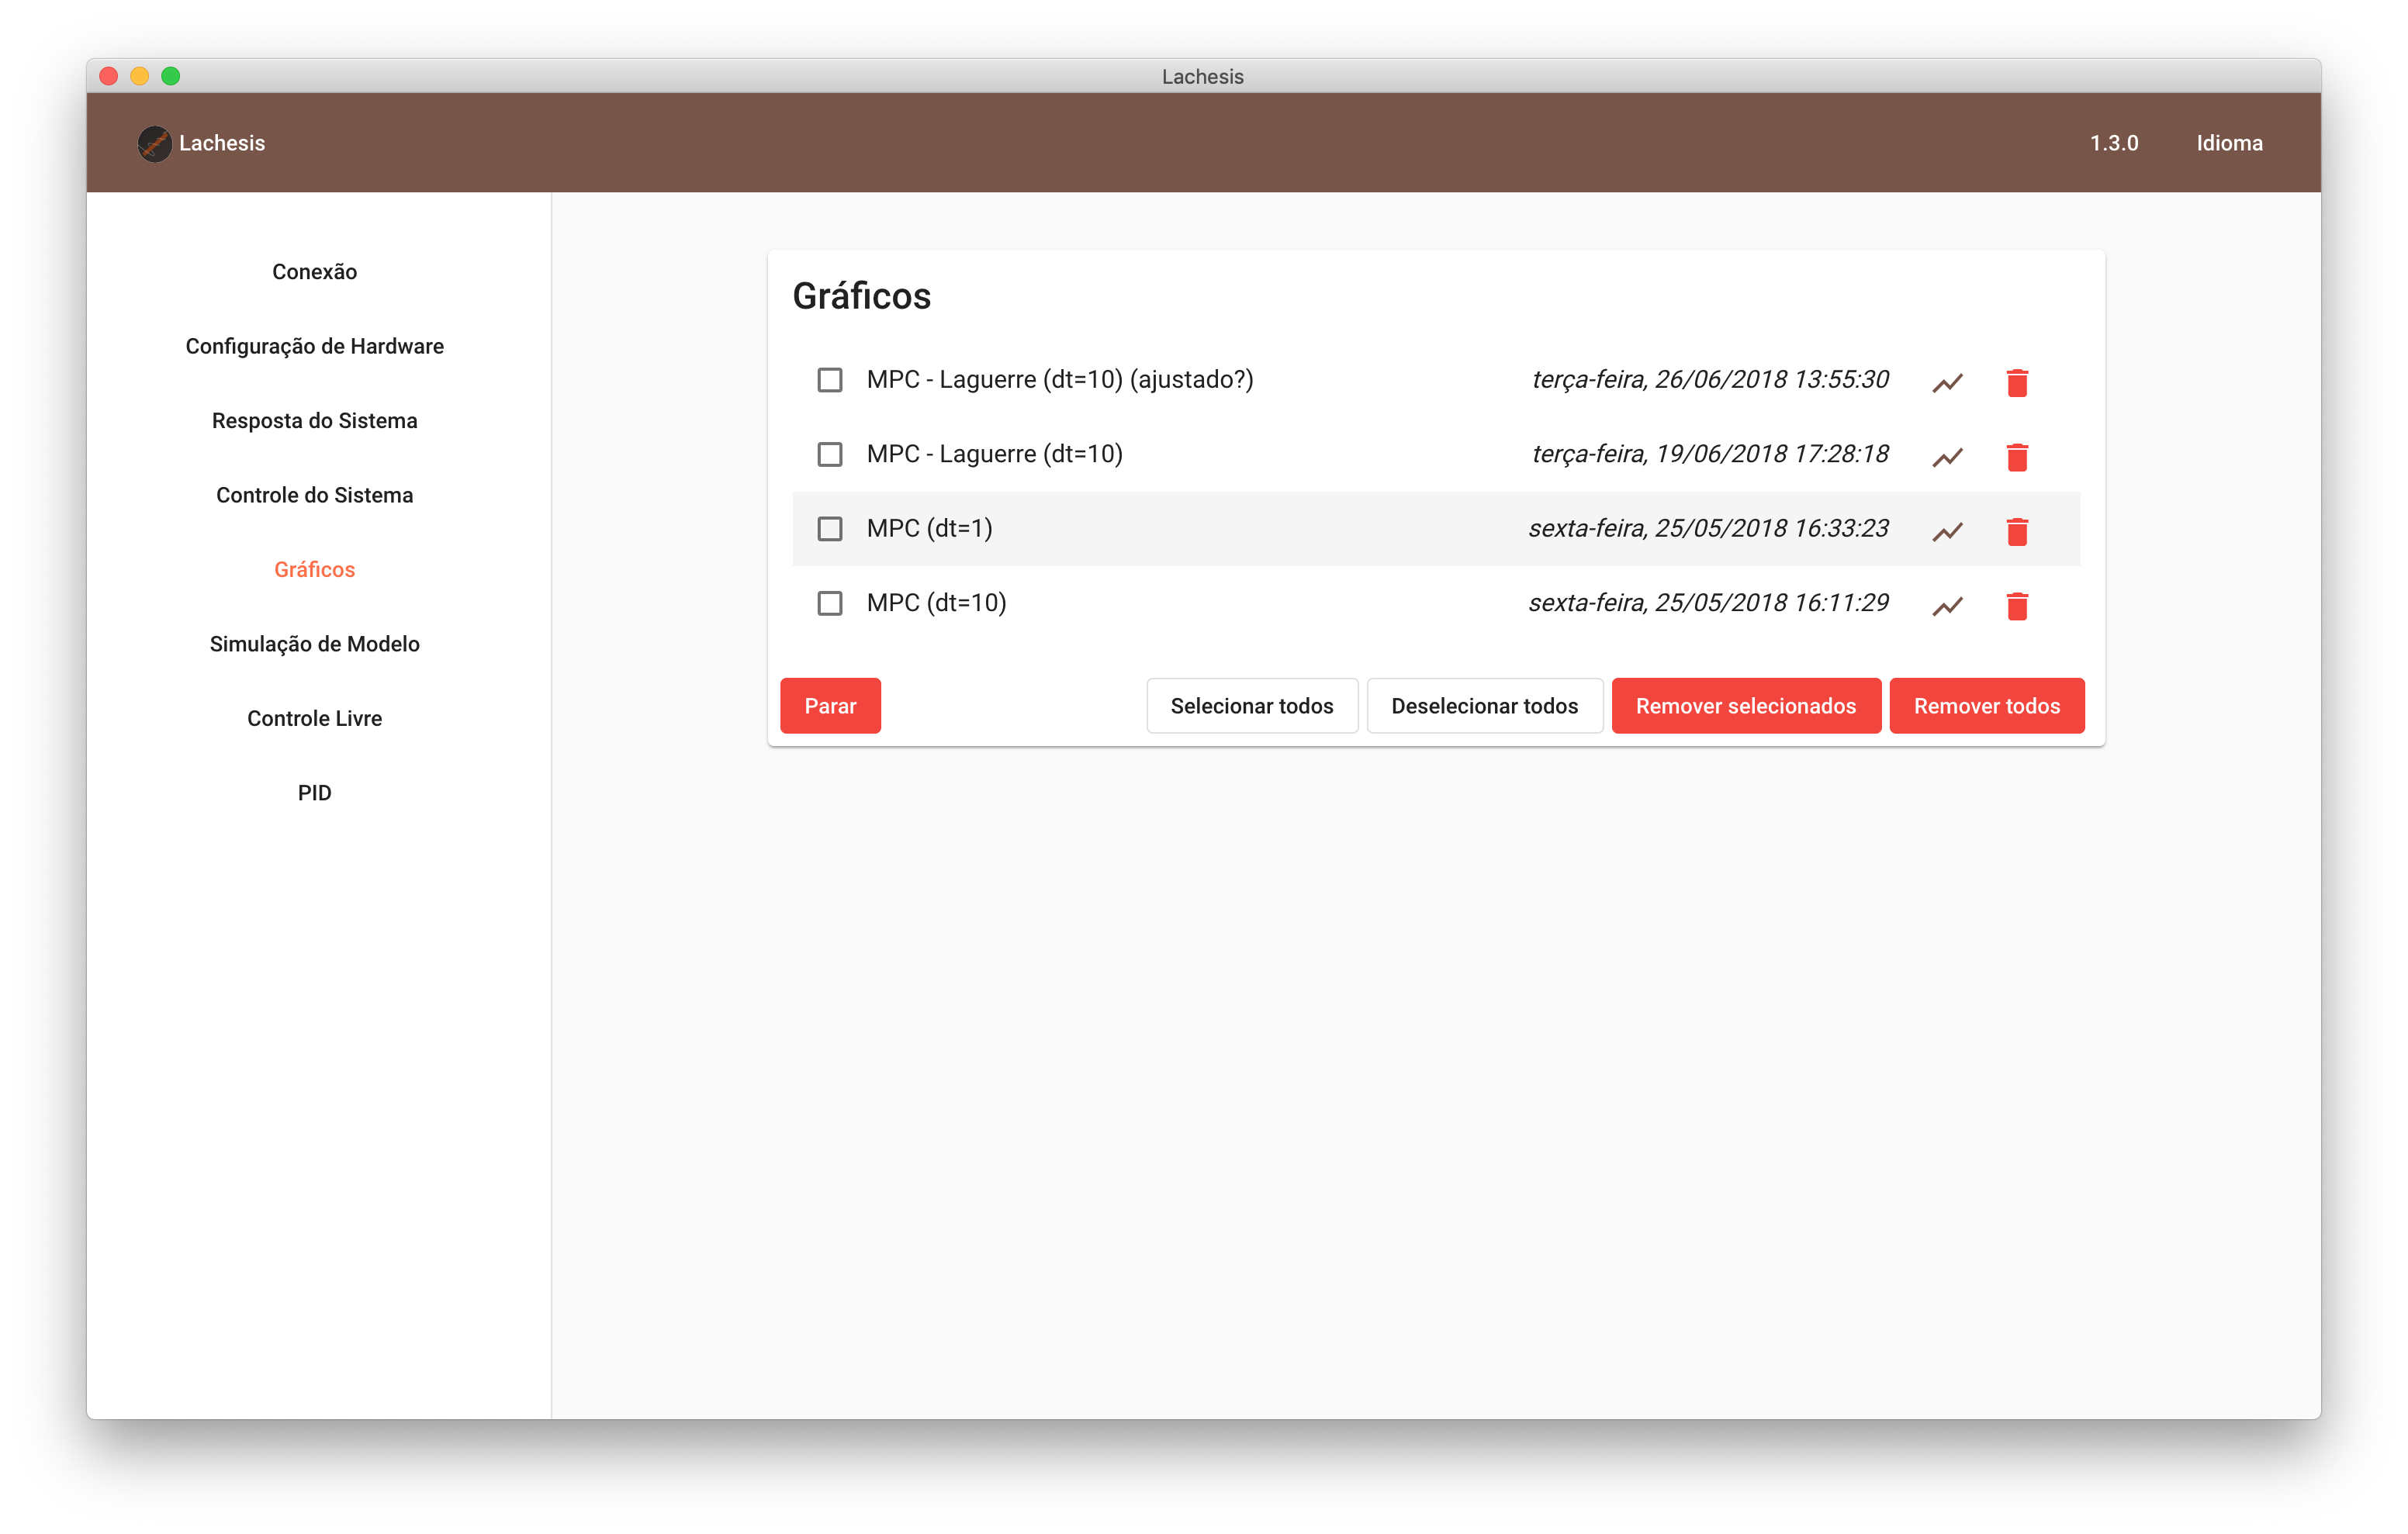
\includegraphics[width=0.9\textwidth]{imgs/graphs1}
    \caption[Módulo Gráficos]{Módulo Gráficos}%
    \label{fig:graphs1}
\end{figure}

Ao clicar em \textit{Exibir} (\img{imgs/show_chart}), a seção \textit{Gráficos}
será exibida. A seção \textit{Exportar} também aparecerá, mas apenas caso o
teste não esteja em execução. A seção \textit{Exportar} é retrátil, se
expandindo ao clicar no título ou botão no lado direito. Na
Figura~\ref{fig:graphs2} pode-se ver a seção expandida. No topo pode-se
selecionar o formato dos dados exportados: \href{https://www.json.org/}{JSON},
\href{https://pt.wikipedia.org/wiki/Comma-separated_values}{CSV} ou
\href{https://www.mathworks.com/help/matlab/import_export/supported-file-formats.html}{MAT}.

\begin{figure}[ht!]
    \centering
    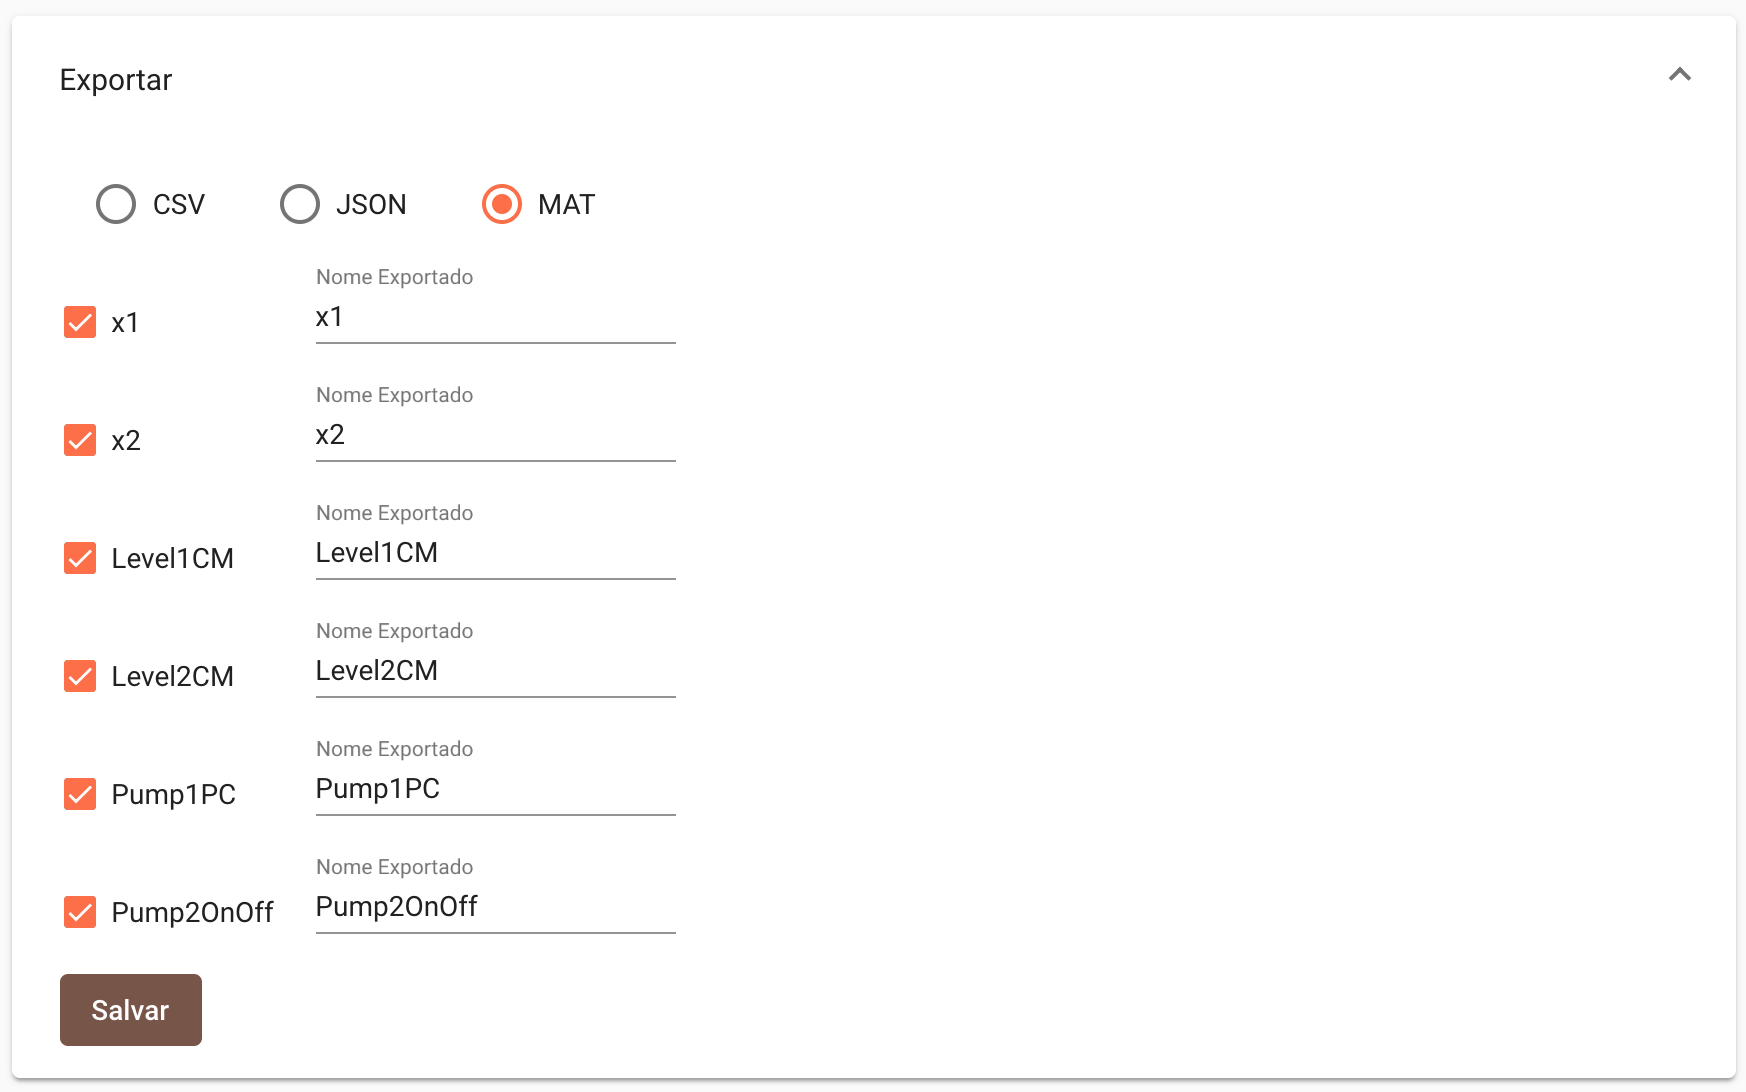
\includegraphics[width=0.9\textwidth]{imgs/graphs2}
    \caption[Exportar dados]{Exportar dados}%
    \label{fig:graphs2}
\end{figure}

Logo em seguida têm-se uma lista de variáveis com \textit{checkboxes} e caixas
de texto. As variáveis com o \textit{checkbox} selecionado serão exportadas, e o
nome definido na caixa de texto será utilizado no arquivo final, ao invés do
nome da variável, permitindo assim que as variáveis sejam renomeadas durante a
exportação. Ao clicar em \textit{Salvar} um arquivo no formato especificado é
gerado e uma janela de salvar arquivo é exibida, permitindo escolher o local
onde o arquivo será salvo.

A seção \textit{Gráficos}, mostradas na Figura~\ref{fig:graphs3}, permite
adicionar gráficos contendo as curvas de uma ou mais variáveis. As variáveis
disponíveis serão as entradas, saídas e aquelas definidas no dicionário
\textit{log}.

\begin{figure}[ht!]
    \centering
    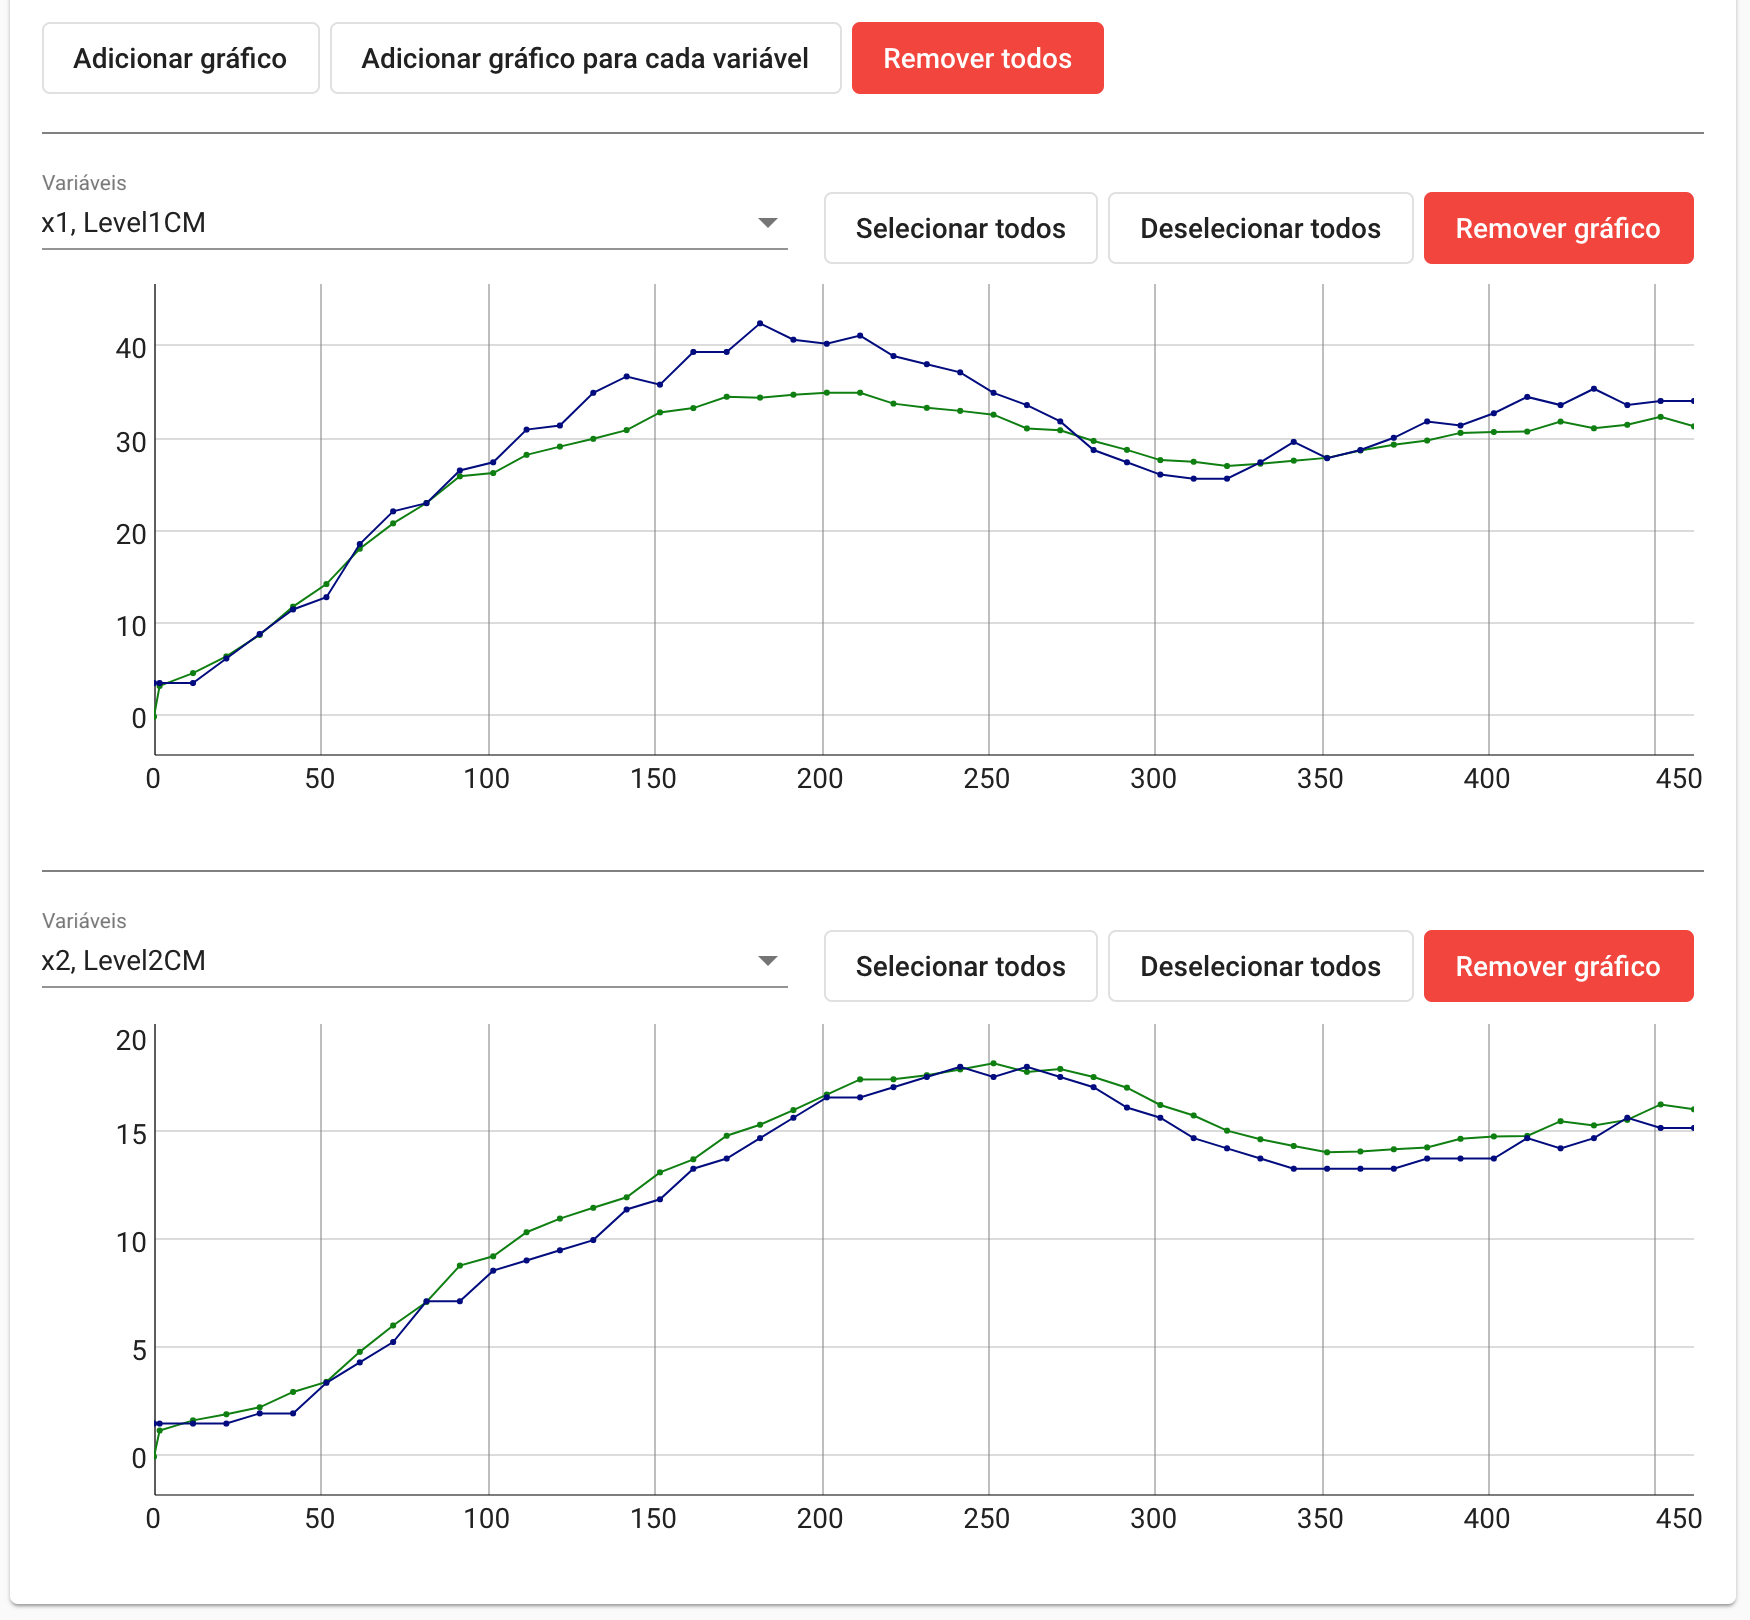
\includegraphics[width=0.9\textwidth]{imgs/graphs3}
    \caption[Gráficos]{Gráficos}%
    \label{fig:graphs3}
\end{figure}

É possível adicionar e remover gráficos sem restrição. Para cada gráfico pode-se
selecionar quais variáveis serão exibidas nele. Algumas funcionalidades de
conveniência estão disponíveis, como a opção de adicionar um gráfico para cada
variável e de selecionar ou deselecionar todas as variáveis em um único gráfico.

Ao passar o \textit{mouse} sobre o gráfico, a legenda é exibida mostrando o nome
de cada curva na mesma cor da linha utilizada no gráfico, além do valor no ponto
atual. O valor eixo \(x\), que sempre representa o tempo em segundos, é exibido
antes de todas as variáveis.

\begin{figure}[ht!]
    \centering
    
\includegraphics[width=0.9\textwidth]{imgs/graphs4}
    \caption[Teste em execução]{Teste em execução}%
    \label{fig:graphs4}
\end{figure}

Quando um teste está em execução, ele é marcado com o símbolo
\img{imgs/running}, como pode ser visto na Figura~\ref{fig:graphs4}. O botão
\textit{Remover} (\img{imgs/remove}) é substituído pelo botão \textit{Parar}
(\img{imgs/stop}). Os gráficos de um teste em execução são atualizados a cada
segundo. Essa atualização requer considerável processamento pelo aplicativo
\textbf{moirai}, sendo recomendado não manter o módulo \textit{Gráficos} aberto
durante a execução de um teste em um computador com baixo poder de
processamento. A lista de gráficos disponíveis também é atualizada a cada
segundo, fazendo com que um teste em execução não seja listado imediatamente,
mas após alguns segundos.

  \cleardoublepage{}
  % !TeX root = document.tex
% !TeX encoding = UTF-8 Unicode

\chapter{Simulação do Modelo}%
\label{chapter:model-simulation}

Esse módulo permite a simulação de um modelo. Na
Figura~\ref{fig:model-simulation} pode-se ver as opções de configuração da
simulação. A simulação suporta modelos contínuos e discretos, em espaço de
estados e função de transferência.

\begin{figure}[ht!]
    \centering
    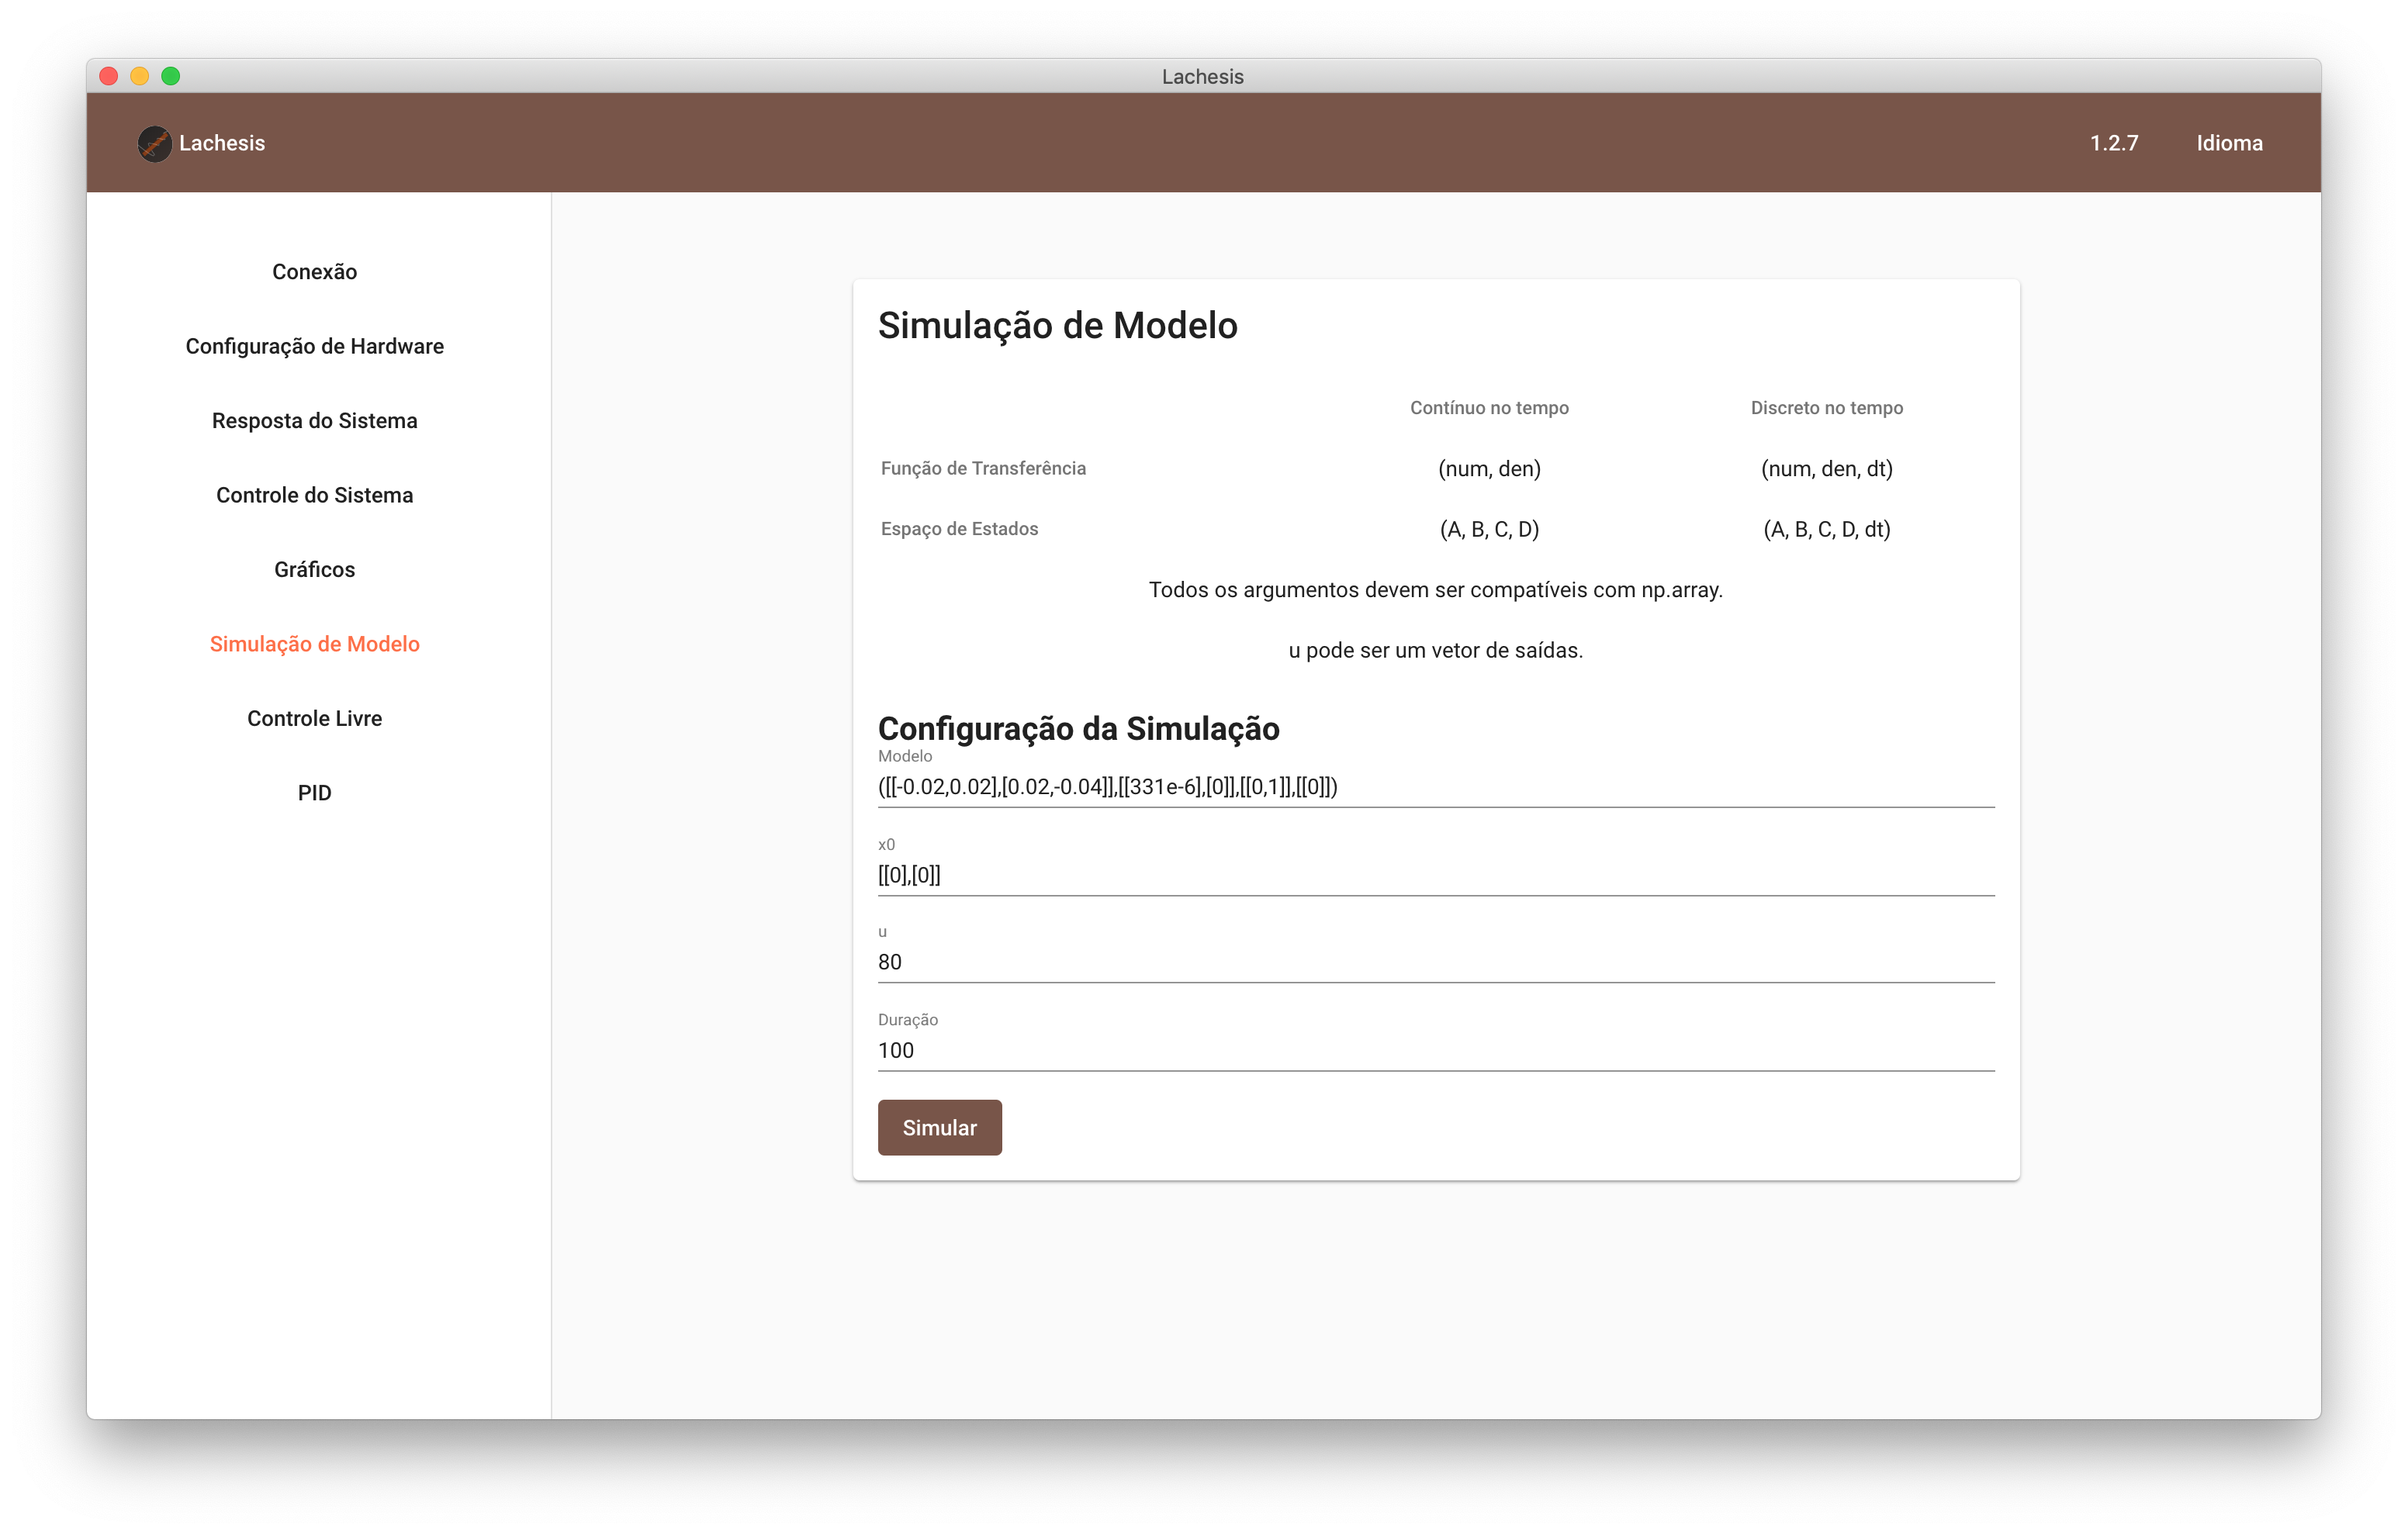
\includegraphics[width=0.9\textwidth]{imgs/model-simulation}
    \caption[Simulação de Modelo]{Simulação de Modelo}%
    \label{fig:model-simulation}
\end{figure}

Caso o modelo não esteja em espaço de estados discreto, ele será convertido para
tal. No caso de modelos contínuos, o tempo de amostragem é calculado como:

\mintinline{python}{dt = max(0.1, float('%.1f' % (max(abs(np.real(vals))) / 5)))}

em que \textit{vals} são os polos do sistema.

Caso o sinal de controle \textit{U} seja informado como um número, ele será
aplicado de forma constante pela duração da simulação. Caso seja um vetor, cada
item será aplicado por uma amostragem, e o valor do campo \textit{Duração} será
ignorado.

Assim, considerando um sistema discreto com \(\delta{}t=5\) segundos, podemos
definir um sinal de controle em rampa de 0 a 100 e retornando a zero como:

\mintinline{python}{[*range(100,5),*range(100,0,-5)]}

Os campos \textit{Modelo}, \textit{x0} e \textit{U} aceitam código
\textit{Python} como entrada, como pode ser visto exemplo anterior. Como a
simulação é sempre feita em espaço de estados discreto, é sempre necessário
informar um \textit{x0} adequado.

O resultado da simulação é salva como um teste, e pode ser vista também no
módulo \textit{Gráficos}, onde é possível exportar os dados.

  \cleardoublepage{}
  % !TeX root = document.tex
% !TeX encoding = UTF-8 Unicode

\chapter{Matemática Computacional}%
\label{chapter:computational-math}

  \cleardoublepage{}
  % !TeX root = document.tex
% !TeX encoding = UTF-8 Unicode

\chapter{Otimização}%
\label{chapter:optimization}

  \cleardoublepage{}

  \nocite{*}
  \printbibliography{}
\end{document}
